%% (Master) Thesis template
% Template version used: v1.4
%
% Largely adapted from Adrian Nievergelt's template for the ADPS
% (lecture notes) project.


%% We use the memoir class because it offers a many easy to use features.
\documentclass[11pt,a4paper,titlepage]{memoir}

%% Packages
%% ========

%% LaTeX Font encoding -- DO NOT CHANGE
\usepackage[OT1]{fontenc}

%% Babel provides support for languages.  'english' uses British
%% English hyphenation and text snippets like "Figure" and
%% "Theorem". Use the option 'ngerman' if your document is in German.
%% Use 'american' for American English.  Note that if you change this,
%% the next LaTeX run may show spurious errors.  Simply run it again.
%% If they persist, remove the .aux file and try again.
\usepackage[english]{babel}

%% Input encoding 'utf8'. In some cases you might need 'utf8x' for
%% extra symbols. Not all editors, especially on Windows, are UTF-8
%% capable, so you may want to use 'latin1' instead.
\usepackage[utf8]{inputenc}

%% This changes default fonts for both text and math mode to use Herman Zapfs
%% excellent Palatino font.  Do not change this.
\usepackage[sc]{mathpazo}

%% The AMS-LaTeX extensions for mathematical typesetting.  Do not
%% remove.
\usepackage{amsmath,amssymb,amsfonts,mathrsfs}

%% NTheorem is a reimplementation of the AMS Theorem package. This
%% will allow us to typeset theorems like examples, proofs and
%% similar.  Do not remove.
%% NOTE: Must be loaded AFTER amsmath, or the \qed placement will
%% break
\usepackage[amsmath,thmmarks]{ntheorem}

%% LaTeX' own graphics handling
\usepackage{graphicx}

%% We unfortunately need this for the Rules chapter.  Remove it
%% afterwards; or at least NEVER use its underlining features.
\usepackage{soul}

%% This allows you to add .pdf files. It is used to add the
%% declaration of originality.
\usepackage{pdfpages}

%% Some more packages that you may want to use.  Have a look at the
%% file, and consult the package docs for each.
%% See the TeXed file for more explanations

%% [OPT] Multi-rowed cells in tabulars
%\usepackage{multirow}

%% [REC] Intelligent cross reference package. This allows for nice
%% combined references that include the reference and a hint to where
%% to look for it.
\usepackage{varioref}

%% [OPT] Easily changeable quotes with \enquote{Text}
%\usepackage[german=swiss]{csquotes}

%% [REC] Format dates and time depending on locale
\usepackage{datetime}

%% [OPT] Provides a \cancel{} command to stroke through mathematics.
%\usepackage{cancel}

%% [NEED] This allows for additional typesetting tools in mathmode.
%% See its excellent documentation.
\usepackage{mathtools}

%% [ADV] Conditional commands
%\usepackage{ifthen}

%% [OPT] Manual large braces or other delimiters.
%\usepackage{bigdelim, bigstrut}

%% [REC] Alternate vector arrows. Use the command \vv{} to get scaled
%% vector arrows.
\usepackage[h]{esvect}

%% [NEED] Some extensions to tabulars and array environments.
\usepackage{array}

%% [OPT] Postscript support via pstricks graphics package. Very
%% diverse applications.
%\usepackage{pstricks,pst-all}

%% [?] This seems to allow us to define some additional counters.
%\usepackage{etex}

%% [ADV] XY-Pic to typeset some matrix-style graphics
%\usepackage[all]{xy}

%% [OPT] This is needed to generate an index at the end of the
%% document.
%\usepackage{makeidx}

%% [OPT] Fancy package for source code listings.  The template text
%% needs it for some LaTeX snippets; remove/adapt the \lstset when you
%% remove the template content.
\usepackage{listings}
\lstset{language=TeX,basicstyle={\normalfont\ttfamily}}

%% [REC] Fancy character protrusion.  Must be loaded after all fonts.
\usepackage[activate]{pdfcprot}

%% [REC] Nicer tables.  Read the excellent documentation.
\usepackage{booktabs}


%% Our layout configuration.  DO NOT CHANGE.
%% Memoir layout setup

%% NOTE: You are strongly advised not to change any of them unless you
%% know what you are doing.  These settings strongly interact in the
%% final look of the document.

% Dependencies
\usepackage{ETHlogo}

% Turn extra space before chapter headings off.
\setlength{\beforechapskip}{0pt}

\nonzeroparskip
\parindent=0pt
\defaultlists

% Chapter style redefinition
\makeatletter

\if@twoside
  \pagestyle{Ruled}
  \copypagestyle{chapter}{Ruled}
\else
  \pagestyle{ruled}
  \copypagestyle{chapter}{ruled}
\fi
\makeoddhead{chapter}{}{}{}
\makeevenhead{chapter}{}{}{}
\makeheadrule{chapter}{\textwidth}{0pt}
\copypagestyle{abstract}{empty}

\makechapterstyle{bianchimod}{%
  \chapterstyle{default}
  \renewcommand*{\chapnamefont}{\normalfont\Large\sffamily}
  \renewcommand*{\chapnumfont}{\normalfont\Large\sffamily}
  \renewcommand*{\printchaptername}{%
    \chapnamefont\centering\@chapapp}
  \renewcommand*{\printchapternum}{\chapnumfont {\thechapter}}
  \renewcommand*{\chaptitlefont}{\normalfont\huge\sffamily}
  \renewcommand*{\printchaptertitle}[1]{%
    \hrule\vskip\onelineskip \centering \chaptitlefont\textbf{\vphantom{gyM}##1}\par}
  \renewcommand*{\afterchaptertitle}{\vskip\onelineskip \hrule\vskip
    \afterchapskip}
  \renewcommand*{\printchapternonum}{%
    \vphantom{\chapnumfont {9}}\afterchapternum}}

% Use the newly defined style
\chapterstyle{bianchimod}

\setsecheadstyle{\Large\bfseries\sffamily}
\setsubsecheadstyle{\large\bfseries\sffamily}
\setsubsubsecheadstyle{\bfseries\sffamily}
\setparaheadstyle{\normalsize\bfseries\sffamily}
\setsubparaheadstyle{\normalsize\itshape\sffamily}
\setsubparaindent{0pt}

% Set captions to a more separated style for clearness
\captionnamefont{\sffamily\bfseries\footnotesize}
\captiontitlefont{\sffamily\footnotesize}
\setlength{\intextsep}{16pt}
\setlength{\belowcaptionskip}{1pt}

% Set section and TOC numbering depth to subsection
\setsecnumdepth{subsection}
\settocdepth{subsection}

%% Titlepage adjustments
\pretitle{\vspace{0pt plus 0.7fill}\begin{center}\HUGE\sffamily\bfseries}
\posttitle{\end{center}\par}
\preauthor{\par\begin{center}\let\and\\\Large\sffamily}
\postauthor{\end{center}}
\predate{\par\begin{center}\Large\sffamily}
\postdate{\end{center}}

\def\@advisors{}
\newcommand{\advisors}[1]{\def\@advisors{#1}}
\def\@department{}
\newcommand{\department}[1]{\def\@department{#1}}
\def\@thesistype{}
\newcommand{\thesistype}[1]{\def\@thesistype{#1}}

\renewcommand{\maketitlehooka}{\noindent\ETHlogo[2in]}

\renewcommand{\maketitlehookb}{\vspace{1in}%
  \par\begin{center}\Large\sffamily\@thesistype\end{center}}

\renewcommand{\maketitlehookd}{%
  \vfill\par
  \begin{flushright}
    \sffamily
    \@advisors\par
    \@department, ETH Z\"urich
  \end{flushright}
}

\checkandfixthelayout

\setlength{\droptitle}{-48pt}

\makeatother

% This defines how theorems should look. Best leave as is.
\theoremstyle{plain}
\setlength\theorempostskipamount{0pt}

%%% Local Variables:
%%% mode: latex
%%% TeX-master: "thesis"
%%% End:


%% Theorem environments.  You will have to adapt this for a German
%% thesis.
%% Theorem-like environments

%% This can be changed according to language. You can comment out the ones you
%% don't need.

\numberwithin{equation}{chapter}

%% German theorems
%\newtheorem{satz}{Satz}[chapter]
%\newtheorem{beispiel}[satz]{Beispiel}
%\newtheorem{bemerkung}[satz]{Bemerkung}
%\newtheorem{korrolar}[satz]{Korrolar}
%\newtheorem{definition}[satz]{Definition}
%\newtheorem{lemma}[satz]{Lemma}
%\newtheorem{proposition}[satz]{Proposition}

%% English variants
\newtheorem{theorem}{Theorem}[chapter]
\newtheorem{example}[theorem]{Example}
\newtheorem{remark}[theorem]{Remark}
\newtheorem{corollary}[theorem]{Corollary}
\newtheorem{definition}[theorem]{Definition}
\newtheorem{lemma}[theorem]{Lemma}
\newtheorem{proposition}[theorem]{Proposition}

%% Proof environment with a small square as a "qed" symbol
\theoremstyle{nonumberplain}
\theorembodyfont{\normalfont}
\theoremsymbol{\ensuremath{\square}}
\newtheorem{proof}{Proof}
%\newtheorem{beweis}{Beweis}


%% Helpful macros.
%% Custom commands
%% ===============

%% Special characters for number sets, e.g. real or complex numbers.
\newcommand{\C}{\mathbb{C}}
\newcommand{\K}{\mathbb{K}}
\newcommand{\N}{\mathbb{N}}
\newcommand{\Q}{\mathbb{Q}}
\newcommand{\R}{\mathbb{R}}
\newcommand{\Z}{\mathbb{Z}}
\newcommand{\X}{\mathbb{X}}

%% Fixed/scaling delimiter examples (see mathtools documentation)
\DeclarePairedDelimiter\abs{\lvert}{\rvert}
\DeclarePairedDelimiter\norm{\lVert}{\rVert}

%% Use the alternative epsilon per default and define the old one as \oldepsilon
\let\oldepsilon\epsilon
\renewcommand{\epsilon}{\ensuremath\varepsilon}

%% Also set the alternate phi as default.
\let\oldphi\phi
\renewcommand{\phi}{\ensuremath{\varphi}}


%% Make document internal hyperlinks wherever possible. (TOC, references)
%% This MUST be loaded after varioref, which is loaded in 'extrapackages'
%% above.  We just load it last to be safe.
\usepackage[linkcolor=black,colorlinks=true,citecolor=black,filecolor=black]{hyperref}


%% Document information
%% ====================
\usepackage{pgfplots} 
\usepackage{gensymb}
\usepackage{hyperref}
\usepackage{float}
\usepackage{amsmath}
\usepackage{algorithm}
\usepackage{algorithmic} 
\usepackage{minted}

\title{StencilFlow: Stencil Dataflow on Reconfigurable Hardware}
\author{A. Kuster}
\thesistype{Bachelor Thesis}
\advisors{Advisors: Prof.\ Dr.\ T. Hoefler, J. de Fine Licht}
\department{Department of Computer Science}
\date{August 20, 2019}

\begin{document}

\frontmatter

%% Title page is autogenerated from document information above.  DO
%% NOT CHANGE.
\begin{titlingpage}
  \calccentering{\unitlength}
  \begin{adjustwidth*}{\unitlength-24pt}{-\unitlength-24pt}
    \maketitle
  \end{adjustwidth*}
\end{titlingpage}

%% The abstract of your thesis.  Edit the file as needed.
\begin{abstract}
Accurate and reliable weather forecast is of vital importance for a broad field of industries and the general public. Highly regular and statically analyzable stencil operators on structured grids are used to numerically solve the partial differential equations of such weather prediction models. This allows optimizations for data re-use while minimizing the high demand of memory bandwidth. Since technology is hitting the power-wall of approximately $1 \frac{Watt}{mm^2}$ for air-cooled CMOS fabrics, while spending a great fraction of the energy for data movement and caching, future high-performance architectures must increase the fraction of energy spent on computations to continue scaling. By implementing custom dataflow architectures on FPGAs, there is a potential to greatly reduce control and data movement overhead. We hope to move a step toward this goal of being more energy efficient compared to the Von-Neuman load/store architecture.\\
In this thesis, we introduce StencilFlow, a framework for mapping stencil programs to FPGAs, offering a complete toolchain from input data analysis, optimization, and simulation, to generation of optimal code for re-programmable devices. We formalize the input program as a directed acyclic graph of streaming modules, and optimize for maximum utilization of on-chip memory and off-chip memory bandwidth. \\
To gain insight into performance metrics and debugging, we develop a model to simulate the stencil program in software. The optimized stencil program is mapped onto FPGA hardware using the DaCe framework. As a realistic use case, we study the COSMO numerical weather forecasting model, currently running on a multi-core and hybrid CPU-GPU architecture. With our framework, high-level users can rapidly implement, optimize, debug, and synthesize arbitrary, large stencil programs onto FPGAs.
\end{abstract}



%% TOC with the proper setup, do not change.
\cleartorecto
\tableofcontents
\mainmatter

%% Your real content! 
\chapter{Introduction}
Accurate and reliable weather forecast is of vital importance for a broad field of industries, as well as the general public. Highly regular and statically analyzable stencil operators \cite{label6} on structured grids  are used to numerically solve the partial differential equations of such weather prediction models. This allows optimizations for data re-use while minimizing the high demand of memory bandwidth. Our collaboration with MeteoSwiss \cite{label37} enables us to apply our theoretical optimization findings to the numerical weather prediction and regional climate model COSMO \cite{label15, label38}. By cooperating closely with Swiss National Supercomputing Center (CSCS) \cite{label39} and the University of Paderborn we gain access to computational hardware resources and intend to figure out together if FPGAs (field-programmable gate arrays) can serve as the next generation accelerator for high-performance weather prediction simulations.


\section{Objectives and Goal}
Nowadays, numerical weather prediction simulations are executed on Von-Neumann architecture \cite{label35} based CPU or GPU clusters \cite{label13}. Since technology is hitting the power-wall of approximately $1 \frac{Watt}{mm^2}$ for air-cooled CMOS fabrics \cite{label1}, high-performance designs should spend a significant amount of that energy for actual computations. Research in the computational field has shown that FPGAs could be a competitive technology in comparison to CPUs \cite{label7}, GPUs \cite{label16} and even ASICs \cite{label8}. By streaming data through the FPGA and therefore greatly reducing control and data movement overhead \cite{label1,label31}, we estimate to be about 8 times (see Appendix A) more energy efficient compared to the load/store architecture. Thus, we seek to implement the numerical model on a state-of-the-art FPGA, the Intel Stratix 10 \cite{label25} using OpenCL \cite{label21} as high-level synthesis (HLS) tool \cite{label18,label36} for increased productivity.


\section{Methods of Investigation / Implementation}
Our theoretical optimization focus lies in the analysis and optimal allocation of resources to reduce the memory bandwidth bottleneck \cite{label2,label3,label28}. By formalizing the input program as a directed graph of streaming modules and formulating it as an optimization problem, we seek to solve it for optimal bandwidth and fast memory usage. To gain insight into performance metrics and for debugging, we develop a model to simulate the stencil program in software. The final step will be to transform this theoretically optimal design onto the FPGA. Studies \cite{label4,label5,label18,label33,label30} have shown that optimization of HLS code is crucial for maximal performance. Therefore, the project is carried out in close collaboration with experts in stencil optimization for different heterogeneous systems (CPU and GPU) \cite{label2,label3,label29, label12,label11,label10,label9} at ETH.


\section{Collaborations}
The outcome of this project highly depends on the symbiosis of partners willing to share their experience, expertise and resources with us. On one hand, we tackle a real-world problem that can help us finding out if our approach can be efficiently scaled up to production scale problems and program sizes. On the other hand, the hardware resources for the synthesis and testing of FPGA designs are very demanding, which is why we have a partner who can provide us with this service. Furthermore, having expert knowledge from other groups involved in high performance FPGA designs helps us a lot to share valuable problem solutions and optimization hints.


\subsection{MeteoSwiss}
MeteoSwiss \cite{label43}, the Federal Office of Meteorology and Climatology located in Zurich, Geneva, Locarno and Payerne is part of the federal administration of Switzerland. Their main task is to constantly create weather forecasts to inform authorities and the general public about upcoming storms and other strong weather phenomena. In addition to that, they provide weather services for civil and the military. \\
MeteoSwiss, together with CSCS are very progressive partners making use of modern, cutting-edge technology. This effort made them the first major national weather service to deploy a GPU-accelerated supercomputer to improve its daily weather forecasts \cite{label44}. \\
We both share the common interest of finding out if FPGAs could be the next technological step forward, which is why we are closely collaborating. This collaboration gives us access to the source code of their current implementation and allows us to directly communicate with experts from MeteoSwiss that are actively involved in the current developments.


\subsection{CSCS}
CSCS \cite{label45}, the Swiss National Supercomputing Center, is the national high-performance computing center of Switzerland. It operates the Piz Daint, one of the world's largest supercomputers (rank 6 in TOP500 at the time of writing, \cite{label42}) in addition to some dedicated computing resources for specific projects and offices of the federal government of Switzerland. \\
Their interest and the associated early purchase of the Stratix 10 FPGA allowed us to do early hands-on test with the hardware and getting valuable insights. In addition to that, high-level synthesis from our high-level OpenCL design to the actual bitstream of the FPGA is a time and resource consuming task. CSCS provides us with Greina and Ault, two large memory cluster computers with integrated FPGA hardware, the required resources for efficient testing and evaluation.


\subsection{University of Paderborn}
The University of Paderborn, Germany, is one of the leading European university in the use of reconfigurable device for high performance applications. With the inauguration of Noctua \cite{label46}, their new cluster computer incorporates 16 nodes with two Intel Stratix 10 FPGA (Bittware 520N) cards each. These cards are interconnected through a optical circuit switch, which gives us the flexibility of potentially splitting the problem and make tests of running it on multiple devices while streaming the necessary data via the dedicated 40Gb/s fiber interconnect. \\
Furthermore, we get expert knowledge from the scientist working in this environment and can share experiences, problems and performance improving design hints. This is especially valuable, since FPGAs are not as main-stream in HPC as CPU and GPUs are. The lack of forum and human resources makes the problem solving more complex. This makes a close collaboration with other people from the same field especially valuable.


\section{Acknowledgement}
I would like to thank my mentor Johannes de Fine Licht for his extraordinary support in this thesis process. Advice given by Professor Torsten Hoefler during the meetings has been of great help in staying on the right track throughout the project. Assistance provided by Carlos Osuna from MeteoSwiss for COSMO related questions was greatly appreciated. I wish to acknowledge the help provided by Hussein Nasser from CSCS by setting up the FPGA cards on Greina and Ault and helping us in case of failure. I am particularly grateful for the assistance given by Tobias Kenter from University of Paderborn in high-level synthesis related questions. Last but not least, Tobias Gysi from ETH Zurich provided me with very valuable inputs from his prior work on the COSMO weather model.
  % done
\chapter{Weather Simulation at MeteoSwiss}


\section{Introduction}
COSMO, the Consortium for Small-scale Modeling \cite{label47}, is an association seeking to develop, improve and maintain a non-hydrostatic limited-area atmospheric model, the COSMO-model. This is the base for many national weather prediction services in Europe. \\
The consortium was established in 1998 by DWD (Germany) and MeteoSwiss (Switzerland). Over the years, weather services and organizations such as ZGeoBw (Germany), ITAF ReMet/CIRA/ARPAE, ARPA Piemont (Italy), HNMS (Greece), IMGW (Poland), IMS (Israel), NMA (Romania) and RHM (Russia) have joined. In addition to meteorological services, there are also academic communities involved, namely the Climate Limited-Area Modeling (CLM) that extended the model for long-term simulations and Universities maintaining their own extensions. The Karlsruhe Insitute for Technology (KIT) extended the model to account for the interactions of gases and aerosols within the state of the atmosphere. \\
The COSMO-model was initially based on DWDs "Lokal-Modell" (Local Model) and further refined and improved in joint collaboration by the COSMO members.


\paragraph{Structure}
A time integration cycle illustrated in figure \ref{fig:cosmo-the-cosmo-model} can be broken down into different tasks and execution phases \cite{label49}. The first steps prepares the input data for processing. The physics step accounts for the physical processes that are not resolved by the 3-dimensional numerical grid (vertical diffusion (turbulences), cloud and precipitation formation (condensation), convection, radiation and soil processes). \\
The dynamical core, consisting of the dynamics and relaxations phase, is the main computational challenge of the weather model. It is formulated in terms of stencil programs applied on the highly regular, three dimensional data grid. Therefore, we focus on this part of the model. \\
The nudging step takes care of the convergence of the computed model values and the actual observations from the observation stations. Finally there is post-processing going on and a cleanup to be ready for the next iteration step.
\begin{figure}[h]
	\centering
	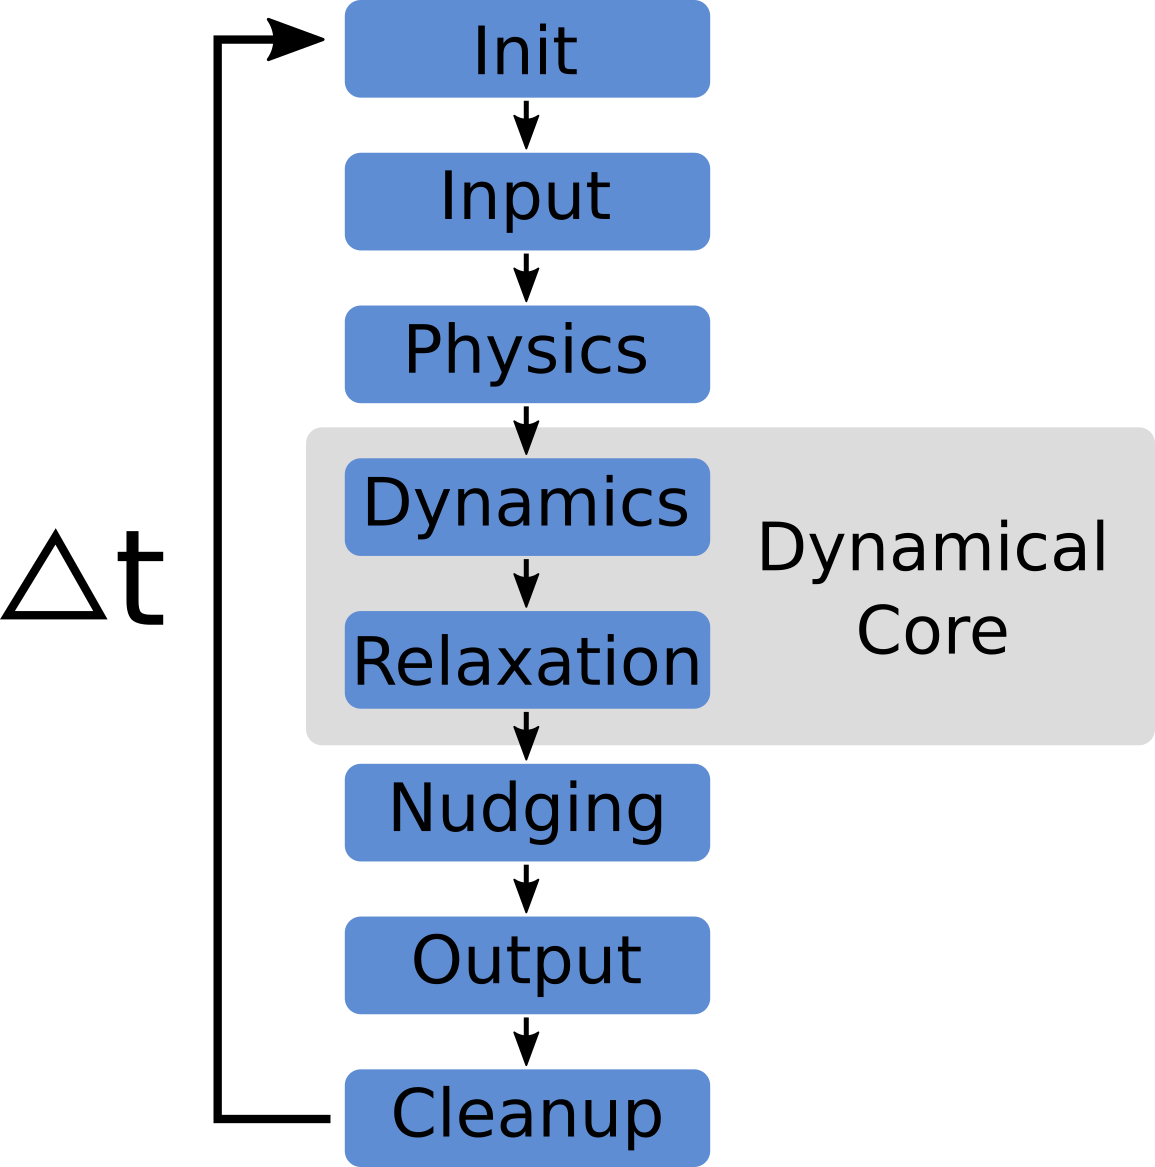
\includegraphics[height=12em]{drawings/cosmo-the-cosmo-model.png}
	\caption{The COSMO Model: Structure of a the time integration interval.}
	\label{fig:cosmo-the-cosmo-model}
\end{figure}


\paragraph{Model Instances (MeteoSwiss Specific)}
MeteoSwiss does not rely on a single instance of the weather model, but rather follows the approach of subdivisions of the forecast into different set of problems \cite{label51}. There are various grid resolution instances and simulation durations shown in figure \ref{fig:cosmo-prediction}, which gives them the ability to better predict longer-term, mid-term and short-term weather constellations in the very challenging topological Alpine region. These grid resolutions define the computational domain of the problem since all stencil operators are applied to each individual grid point.
\begin{figure}[h]
	\centering
	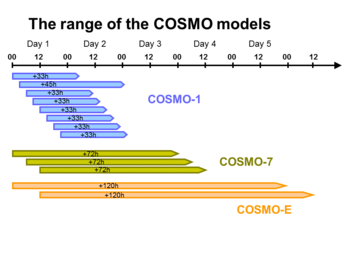
\includegraphics[height=12em]{images/cosmo-prediction.png}
	\caption{Range of COSMO models with their forecast horizon and number of runs per day. \textit{meteoswiss.admin.ch}}
	\label{fig:cosmo-prediction}
\end{figure}


\subparagraph{COSMO-1}
The COSMO-1 instance is a high-resolution version with a grid-box size of 1.1km (0.01\degree) spread over the Alpine region. It is able to predict precipitation, temperature, wind as seen in figure \ref{fig:cosmo-1} and numerous other meteorological parameters. The number of grid points is 1158x774 horizontally and 80 in the vertical dimension. The model topography reaches 4268 meters above sea level. Every grid point is updated in a time integration interval of 10 seconds.
\begin{figure}[h]
	\begin{minipage}{.24\columnwidth}
		\centering
		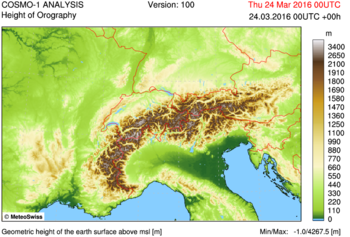
\includegraphics[height=5em]{images/cosmo-1-general.png}
		\label{fig:cosmo-1-general}
	\end{minipage}
	\begin{minipage}{.24\columnwidth}
		\centering
		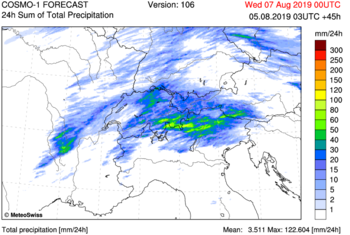
\includegraphics[height=5em]{images/cosmo-1-precipitation.png}
		\label{fig:cosmo-1-precipitation}
	\end{minipage}
	\begin{minipage}{.24\columnwidth}
		\centering
		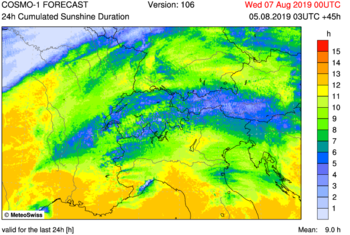
\includegraphics[height=5em]{images/cosmo-1-sunshine-duration.png}
		\label{fig:cosmo-1-sunshine-duration}
	\end{minipage}
	\begin{minipage}{.24\columnwidth}
		\centering
		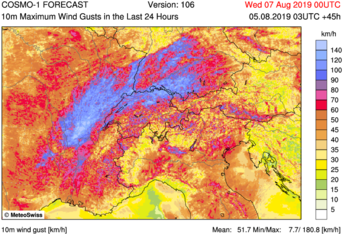
\includegraphics[height=5em]{images/cosmo-1-10m-max-wind-guts.png}
		\label{fig:cosmo-1-10m-max-wind-guts}
	\end{minipage}
	\caption{COSMO-1 example model parameters: Height of Orography, Sum of total Precipitation (Prediction), 24h Sum of Sunshine Hours (Prediction), 10m Above Ground Maximum Wind Guts (Past) (from left to right), \textit{meteoswiss.admin.ch}}
	\label{fig:cosmo-1}
\end{figure}


\subparagraph{COSMO-E}
The COSMO-E models purpose is to improve the reliability of the short to medium range forecast for highly localized weather events. It is a collection of 21 different forecasts that are being executed twice a day. \\
It covers the whole Alpine region, but with a lower resolution in comparison to the COSMO-1 instance. It uses grid box sizes of 2.2km and 582x390 horizontal grid points and 60 vertical layers.
\begin{figure}[h]
	\begin{minipage}{.32\columnwidth}
		\centering
		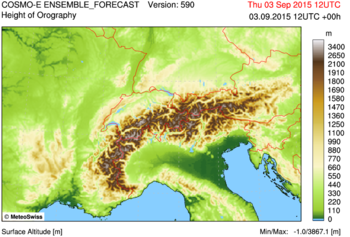
\includegraphics[height=8em]{images/cosmo-m-general.png}
		\label{fig:cosmo-m-general}
		\vspace{-1em}
	\end{minipage}
	\begin{minipage}{.32\columnwidth}
		\centering
		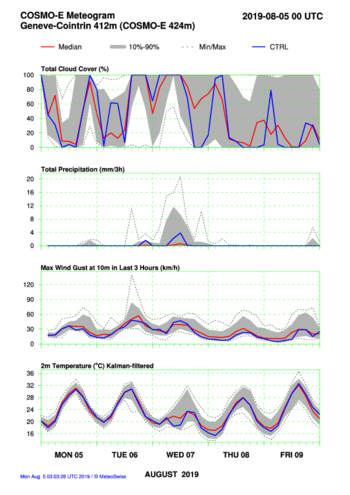
\includegraphics[height=8em]{images/cosmo-m-meteograph-geneve.png}
		\label{fig:cosmo-m-meteograph-geneve}
	\end{minipage}
	\begin{minipage}{.32\columnwidth}
		\centering
		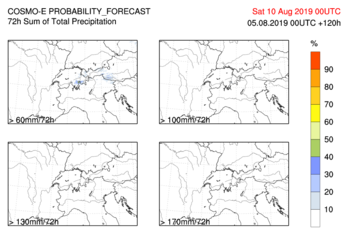
\includegraphics[height=8em]{images/cosmo-m-probability-forecast.png}
		\label{fig:cosmo-m-probability-forecast}
		\vspace{-1em}
	\end{minipage}
	\caption{COSMO-E example model parameters: Height of Orography, Meteogram for Geneva-Cointrin, Probability Forecast (from left to right), \textit{meteoswiss.admin.ch}}
\end{figure}


\subparagraph{COSMO-7}
The COSMO-7 instance with a grid box size of 6.6km (0.06\degree) is a low-resolution version with the aim of covering central and western Europe. The predictions are being run four times a day over a grid of size 393x338 horizontally and 60 vertical units.
\begin{figure}[h]
	\begin{minipage}{.32\columnwidth}
		\centering
		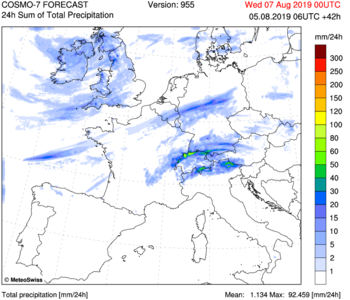
\includegraphics[height=8em]{images/cosmo-7-precipitation.png}
		\label{fig:cosmo-7-precipitation}
	\end{minipage}
	\begin{minipage}{.32\columnwidth}
		\centering
		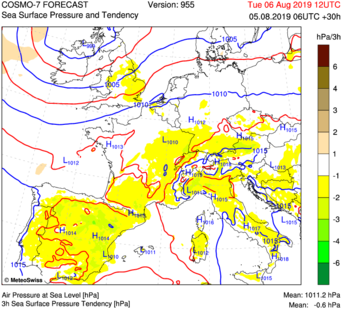
\includegraphics[height=8em]{images/cosmo-7-forecast.png}
		\label{fig:cosmo-7-forecast}
	\end{minipage}
	\begin{minipage}{.32\columnwidth}
		\centering
		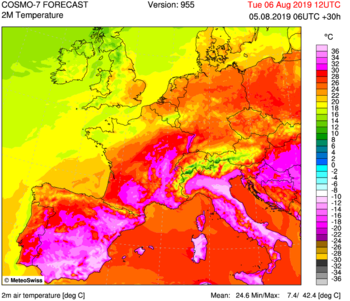
\includegraphics[height=8em]{images/cosmo-7-temperature.png}
		\label{fig:cosmo-7-temperature}
	\end{minipage}
	\caption{COSMO-7 example model parameters: Height of Orography, Air Pressure at Sea Level, 2m Air Temperature (from left to right), \textit{meteoswiss.admin.ch}}
\end{figure}


\subparagraph{Specialized Seasonal Instances}
There exists also seasonal model instances for specific problems, such as the COSMO-ART, which computes the pollen concentration of alder, birch, grasses and ragweed pollen, and is in service from February till end of September).






\subsection{Compute Hardware of MeteoSwiss}

\paragraph{History}
Since simulation-dependent scientific areas can improve their prediction accuracies by increasing model complexity and resolution, they were able to benefit a lot from the exponential increase in compute power over the last couple of decades. This can be well observed by the increase in node and core counts of MeteoSwiss' cluster compute infrastructure \cite{label52}. 
\begin{itemize}
	\item 1999–2007: "Prometeo", NEC SX-5, vector processor, 16 nodes
	\item 2007-2012: 
	\begin{itemize}
		\item "La Dôle", Cray XT4, AMD Opteron quad-core Barcelona 2.3 GHz, 160 nodes (640 cores) 
		\item Piz Buin 	Cray XT4 	AMD Opteron quad-core Barcelona 2.3 GHz, 264 nodes (1,056 cores) 
	\end{itemize}
	\item from 2012
	\begin{itemize}
		\item "Monte Lema", Cray XE6, AMD Opteron 12-core Magny-Cours 2.1 GHz, 336 nodes (4,032 cores) 
		\item "Albis", Cray XE6, AMD Opteron 12-core Magny-Cours 2.1 GHz, 144 nodes (1,728 cores) 
	\end{itemize}
	\item from 2015
	\begin{itemize}
		\item "Kesch" and "Es-cha", Cray CS-Storm, Intel Haswell-EP + Nvidia Tesla K80 GPUs (heterogenous system)
	\end{itemize}
\end{itemize}

\subparagraph{Today}
MeteoSwiss together with CSCS are very ambitious and progressive institutions by keeping up with the pace of technology development. This can be observed very well by the hardware details of Kesch and Es-cha, which was the first cluster computer of a national weather forecast service using a heterogeneous combination of CPUs and GPU compute cards for performance increase \cite{label53}. 
\begin{itemize}
	\item "Kesch and Es-cha": 12 hybrid compute nodes consisting of \cite{label54}:
	\begin{itemize}
		\item 2 Intel Haswell E5-2690v3 2.6 GHz 12-core CPUs per node (total of 24 E5-2690v3 processors)
		\item 256 GB 2133 MHz DDR4 memory per node (total of 3 TB)  
		\item 8 NVIDIA Tesla K80 GPU devices per node (total of 192 GPUs)    
	\end{itemize}
\end{itemize}
\begin{figure}[h]
	\begin{minipage}{.5\columnwidth}
		\centering
		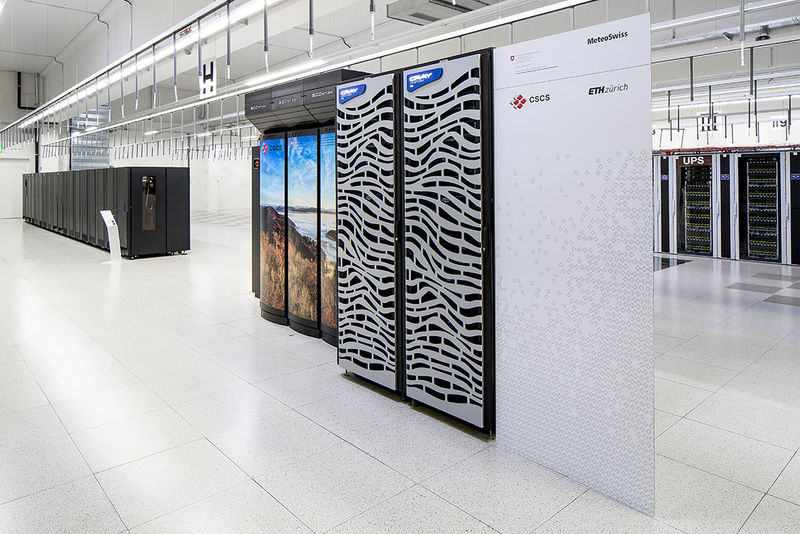
\includegraphics[height=8em]{images/meteoswiss-computer1.jpg}
		\label{fig:meteoswiss-computer1}
	\end{minipage}
	\begin{minipage}{.5\columnwidth}
		\centering
		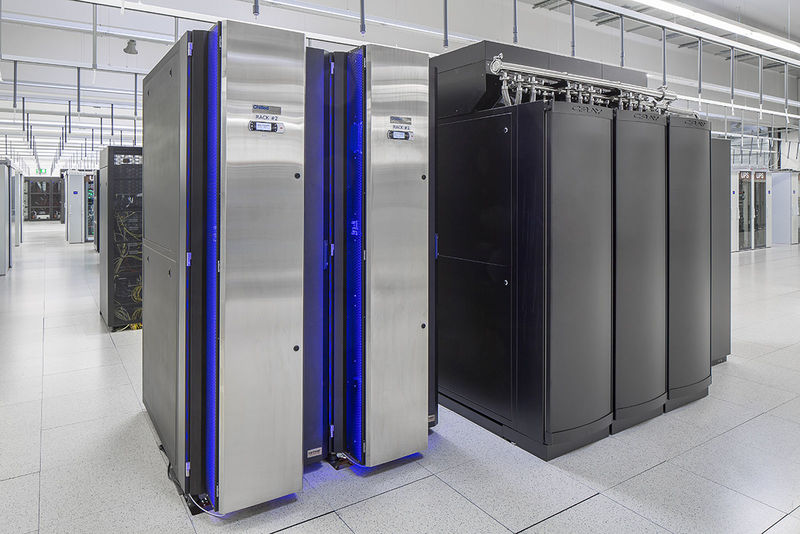
\includegraphics[height=8em]{images/meteoswiss-computer2.jpg}
		\label{fig:meteoswiss-computer2}
	\end{minipage}
	\caption{Kesch and Es-cha, the two compute clusters dedicated for the MeteoSwiss weather prediction. \textit{cscs.ch}}
\end{figure}


\subsection{Current Limitation}
Even thought the transistor density and the number of computations per time unit is still increasing, the memory subsystem can not keep up. Stencil computations on structured grids, which COSMOs dynamical core consists of are heavily memory bound. Figure \ref{fig:dycore-estimate-complexity} illustrates the abstraction levels from the dynamical core as a stencil program down to the actual compute stencils with their corresponding data field accesses. This means that the ratio of compute operations compared to the number of data field accesses is very low. This fact limits the effectiveness of the upgrade of compute resources, since many compute elements are idling and waiting for data to be transfered to them. \\
STELLA \cite{label2} and MODESTO \cite{label3} try to solve or mitigate this problem by optimizing the stencil programs to optimally use the cache hierarchy and therefore reducing the stress on the actual memory bandwidth. 
\begin{figure}[H]
	\centering
	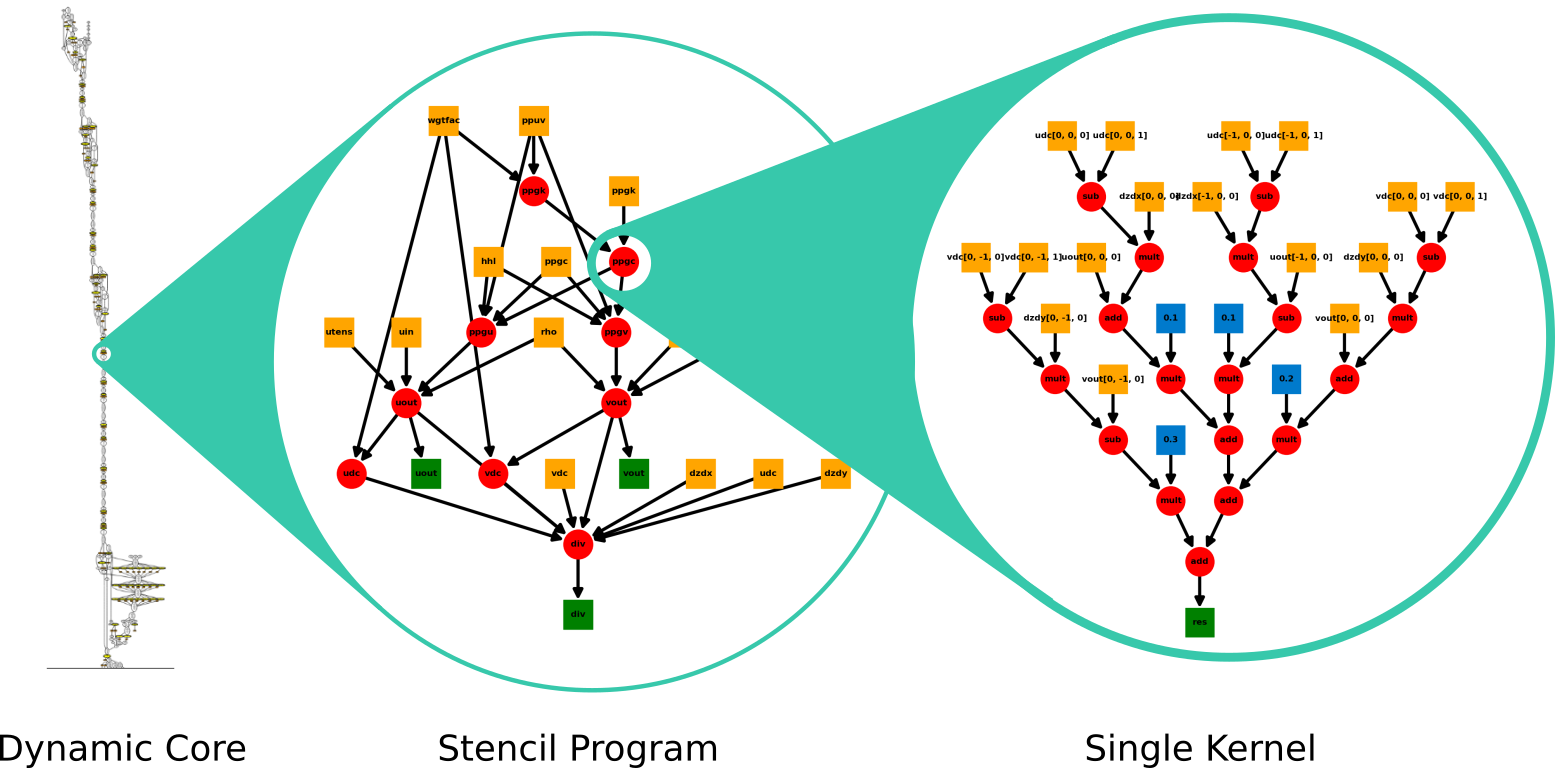
\includegraphics[width=.7\textwidth]{drawings/dycore-estimate-complexity.png}
	\caption{Overview of the total complexity and number of memory accesses given the different hierarchy layers of abstraction.}
	\label{fig:dycore-estimate-complexity}
\end{figure}


\subparagraph{Benefit of FPGA}
This is exactly where the strength of FPGAs lies in. The freedom of not having fixed, hard-wired cache hierarchies, but rather access to spread the fast memory resources in a fine-grained manner such that the overall design profits the most. This increases the actual number of computations per unit time. The next chapter is dedicated to our solution approach and how we intend to implement this in practice. % done
\chapter{StencilFlow Architecture Model}
One the one hand, field programmable gate arrays give us much higher flexibility compared to traditional computed devices such as central progressing units or graphics processing units. On the other hand, a good strategy and knowledge about the underlying hardware is required in order to make use of this additional degrees of freedom.\\
This section is dedicated to outline theoretical aspects of the overall strategy we are proposing. This includes the transformation from the abstracted high-level theoretical input to the mapping onto the actual hardware resources. 



\section{Application Specific Dataflow for Weather Codes}
Kernel computations on structured grids usually impose high stress on data movement since the amount of actual computations is rather low. Therefore we seek to transform the problem to a single, deep pipeline. This allows us to directly forward the intermediate result of a compute unit to the next   unit, instead of transferring it back to slow memory (or some intermediate cache) and later fetch it again. This optimization technique is widely used in hardware designs and not only increases the efficient usage of the resources, but can also save energy by not involving the lower memory hierarchy.\\
As we will see later on, larger designs with more complex dependencies might impose constraints such that we are not always able to directly forward the result to the next processing unit. Therefore we have to statically analyze where and in which size we have to allocate buffers for temporary storing the intermediate results. Since fast memory is limited, we have to find a good strategy to decide whether or not to use fast memory for a buffer allocation or sacrifice memory bandwidth and swap the buffer out to slow memory.


\subsection{Example Walk-through}
To better understand what this means in practice, we will go through the transformation of a simple two kernel example stencil program and its transformation to a fully pipelined design. \\
The stencil program illustrated in figure \ref{fig:approach-stencil-program} consists of three input data arrays (inA, inB, inC), a first kernel kernelA reading from inA and inB a second kernel kernelB reading from inC and kernelA. The final result is the output of kernelB. \\
\begin{lstlisting}[showstringspaces=false, frame=single, language=Python, label={lst:example-stencil-program}]     
inputs: inA, inB, inC
outputs: kernelB
kernels:
kernelA[i,j,k] = (inA[i,j,k]+inA[i,j,k+1])*inB[i,j,k]
kernelB[i,j,k] = (1.0-inC[i,j,k])*kernelA[i,j,k]
\end{lstlisting}
\begin{figure}[h]
	\centering
	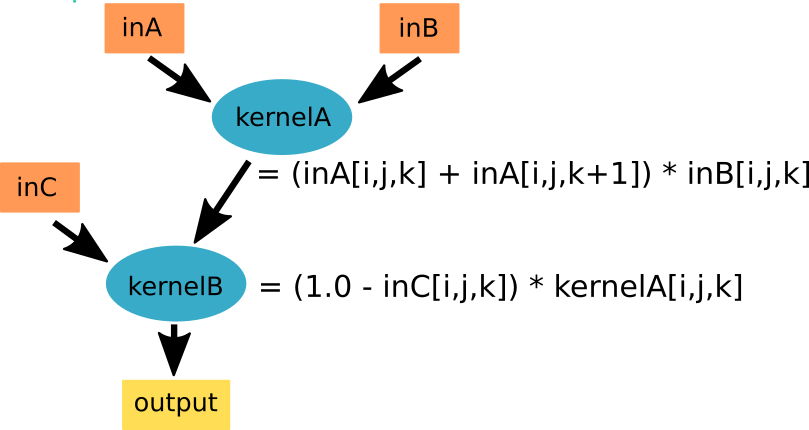
\includegraphics[height=12em]{drawings/approach-stencil-program.png}
	\caption{Example stencil program in high-level data flow representation.}
	\label{fig:approach-stencil-program}
\end{figure}

To avoid storing results of kernelA back to memory, we can directly forward the result to kernelB as illustrated in listing.
\begin{lstlisting}[showstringspaces=false, frame=single, language=Python, label={lst:example-stencil-program-substituted}]     
inputs: inA, inB, inC
outputs: kernelB
kernels:
kernelB[i,j,k] = (1.0 - inC[i,j,k])*(inA[i,j,k] +
                 inA[i,j,k+1])*inB[i,j,k]
\end{lstlisting}
This expression can then be laid down in a pipeline manner by following the mathematical precedence rule of the operation shown in figure \ref{fig:approach-stencil-program-pipeline}.
\begin{figure}[h]
	\centering
	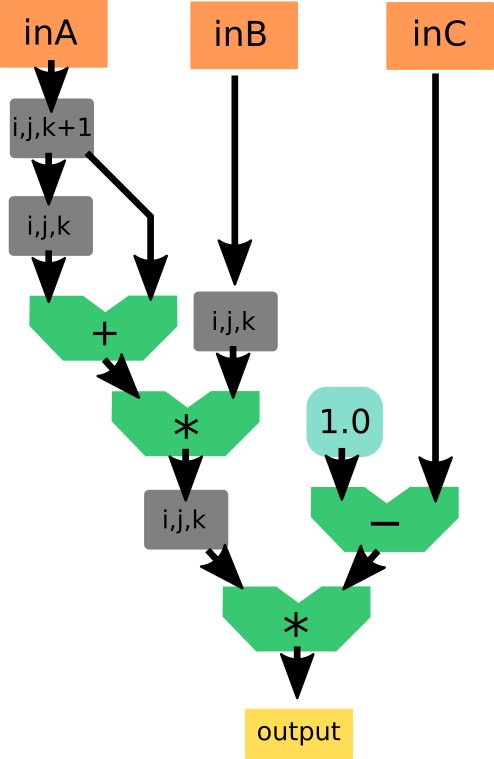
\includegraphics[height=16em]{drawings/approach-stencil-program-pipeline.png}
	\caption{Example stencil program visualized as a pipeline.}
	\label{fig:approach-stencil-program-pipeline}
\end{figure}
Since we are reading two fields from inA with an offset of one, we have to add a stage where we buffer the element at [i,j,k] first in order to be able to read both data elements simultaneously. \\
When we look from a higher level at the pipeline again, illustrated in figure \ref{fig:approach-stencil-program-pipeline-annotated}, we can see the major components:
\begin{itemize}
	\item Inputs: the input data arrays: inA, inB, inC
	\item Kernels: the two compute kernels: kernelA, kernelB
	\item Output: the output data store with the compute result: output
	\item a channel that transfers data from the first to the second kernel
\end{itemize}

\begin{figure}[h]
	\centering
	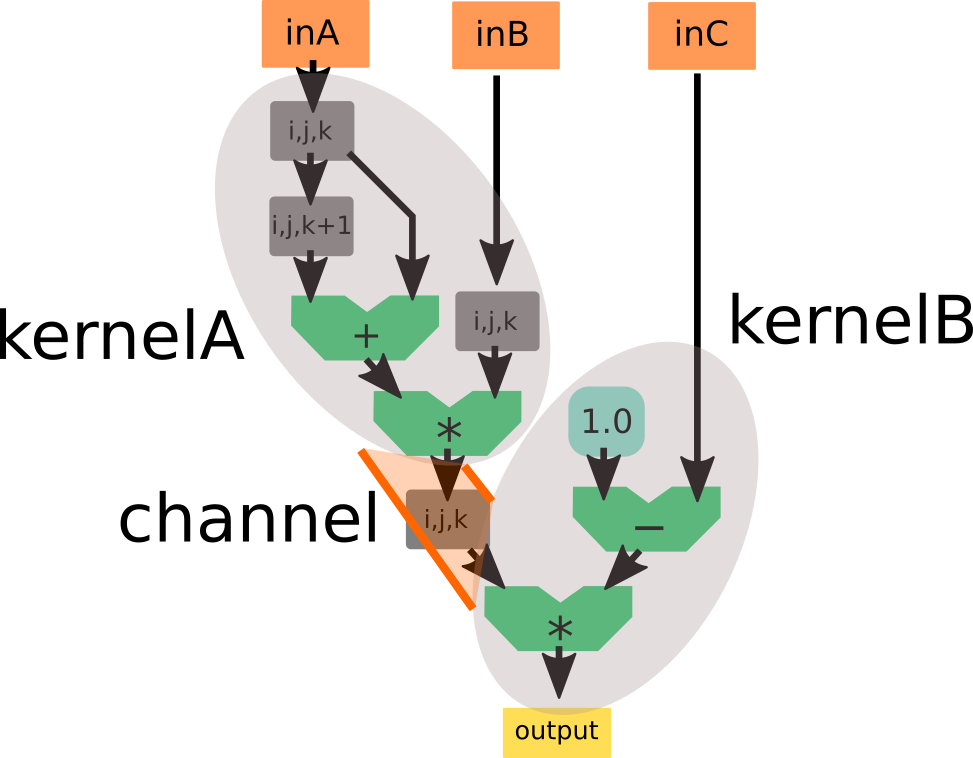
\includegraphics[height=16em]{drawings/approach-stencil-program-pipeline-annotated.png}
	\caption{Example stencil program with additional annotation about the structure of kernels and channels connecting the kernels.}
	\label{fig:approach-stencil-program-pipeline-annotated}
\end{figure}
As we will see later on, this structure builds the foundation for further analysis.


\subsection{Reason}
There are several reasons why we think that deep pipelining is the right choice. First, todays FPGAs are very well suited and optimized to generate highly efficient and higher-frequency designs compared to earlier re-programmable hardware logic designs \cite{label55,label56}. In addition, the incorporated hard compute units have a raw peak performances of 10 TFLOP/s of 32-bit single precision floating point compute performance.\\  
Furthermore, pipelining can save us a lot of data movements since we can directly forward the result of the previous computation to the next compute unit. This can significantly increase performance in case of memory bottlenecks and the idling time associated with it.


\paragraph{}
We conclude that the actual problem is about optimal allocation of the different resources for maximizing the overall throughput. This brings us to the question of, given an stencil program, which and how much resources are required to implement it efficiently in hardware. The next section is dedicated to this input problem analysis. 





\section{Analysis}
This section is dedicated to find and formalize the key metrics for transforming an input problem to a fully pipelined design. We reason about how different patterns of the input program require certain resources such as buffer space and generalize this in order to make these analysis steps fully automatic by StencilFlow.\\
As we have seen in the previous section, it naturally makes sense to split the stencil program into inputs, kernels and outputs. We will therefore first look at the individual kernels and later on use the information and insights gained from this to reason about the whole stencil program.


\subsection{Kernel}
The base of a kernel consists of a kernel string or mathematical expression, the actual stencil. We are dealing with shift-invariant stencils that can read from a neighborhood of the center element [i,j,k] to produce the result for the data element at [i,j,k]. This stencil pattern is then applied for the elements in the grid.\\
The key metrics we are interested in is the latency of a single computation given the latency of each individual operation and the amount of buffer space required such that we do not have to re-fetch the same data element for the stencil twice. We will refer to this as the internal buffer and derive the formula for its size in this section. \\


\paragraph{Stencil}
Shift-invariant stencils are operators that perform element-wise computation of a function F over a fixed neighborhood S. Therefore they can be element-wise applied to each location of the data grid as illustrated in figures \ref{fig:model-stencil-general} and \ref{fig:model-stencil2}. 

\begin{minted}{python}
for i=1..N
  for j=1..M
    out(i,j) = F(S(i,j))
\end{minted}
\begin{align}
\text{S}(i,j) = \text{in}(u,v)
\text{, (u,v)} \in \{(i,j), (i,j-1), (i,j+1), (i-1,j), (i+1,j)\}
\end{align}
\begin{align}
\text{F: } \mathbb{R}^{|S|} \rightarrow \mathbb{R}
\end{align}



\begin{figure}[h]
	\begin{minipage}{.5\columnwidth}
		\centering
		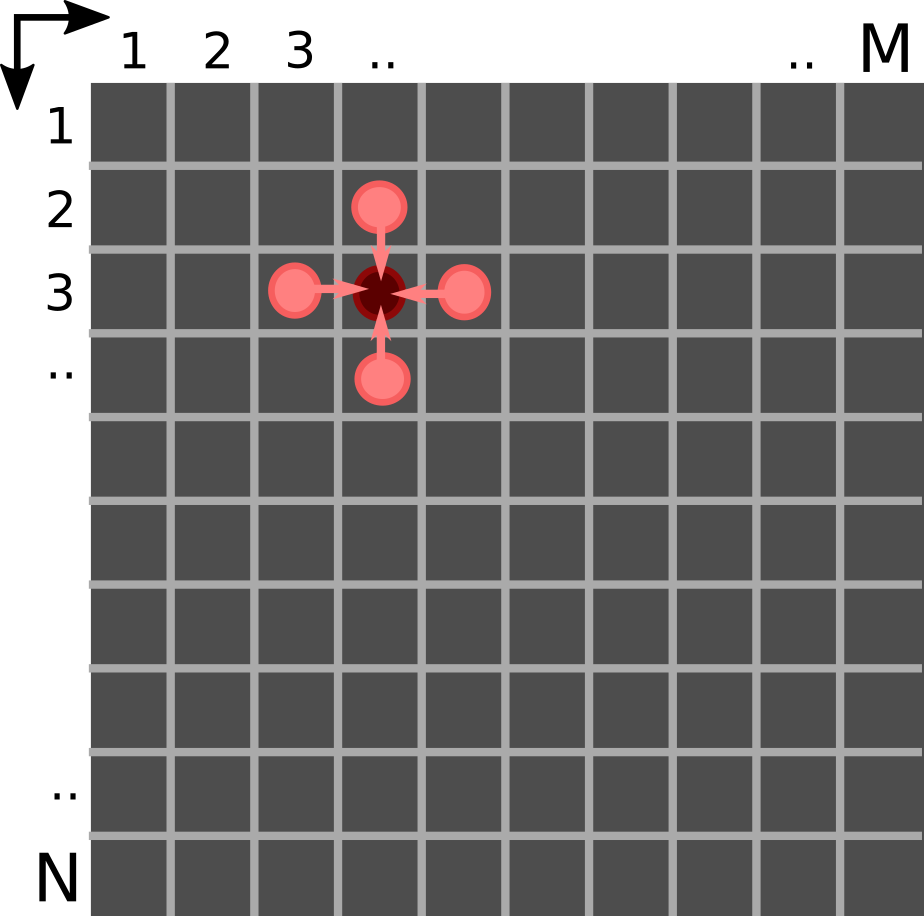
\includegraphics[height=16em]{drawings/model-stencil-general.png}
		\caption{A two dimensional stencil laid out on a two dimensional grid.}
		\label{fig:model-stencil-general}
		\vspace{1em}
	\end{minipage}
	\begin{minipage}{.5\columnwidth}
		\centering
		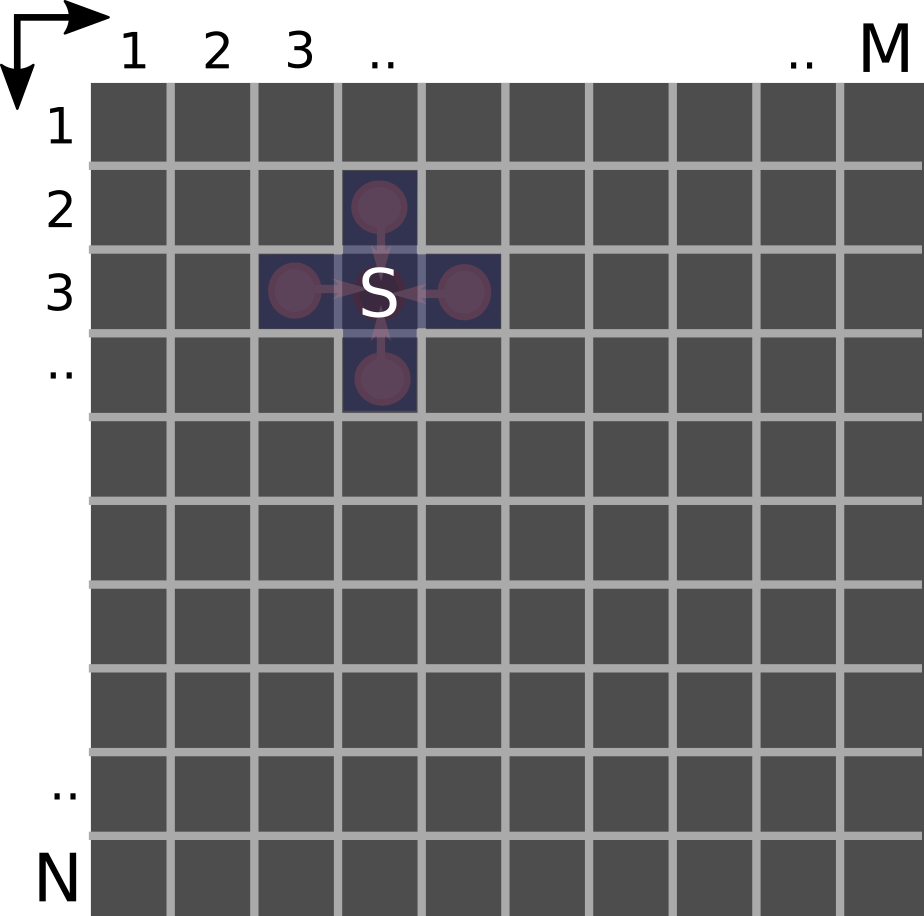
\includegraphics[height=16em]{drawings/model-stencil-neighbourhood-array.png}
		\caption{A two dimensional stencil laid out on a two dimensional grid with emphasized neighborhood S.}
		\label{fig:model-stencil2}
	\end{minipage}
\end{figure}



\subparagraph{Boundary Conditions}
At the boundary of the grid shown in figure \ref{fig:model-boundary-condition1}, some accesses of the neighborhood might be out-of-bound. For this special case, there are different strategies that can be applied to pad the grid shown in figure \ref{fig:model-boundary-condition2}. \\
The most commonly used ones are constant, copy and interpolation boundary conditions. The constant boundary condition assigns a pre-defined constant value to each out-of-bound data access. The copy boundary condition copies the value of the last valid access field and the interpolation boundary condition interpolates the value from some neighborhood around the boundary (e.g. polynomial of degree one or two).
\begin{figure}[H]
	\begin{minipage}{.5\columnwidth}
		\centering
		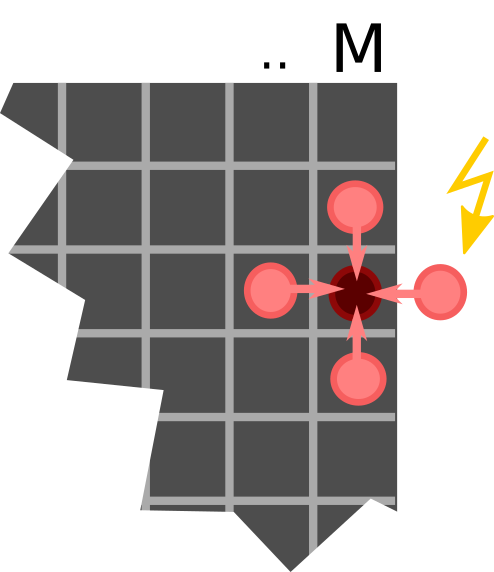
\includegraphics[height=12em]{drawings/model-boundary-condition1.png}
		\caption{Example case of a field access outside of the data array.}
		\label{fig:model-boundary-condition1}
		\vspace{1em}
	\end{minipage}
	\begin{minipage}{.5\columnwidth}
		\centering
		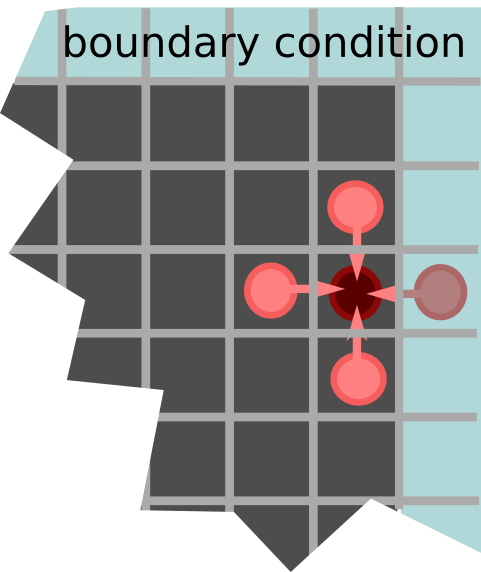
\includegraphics[height=12em]{drawings/model-boundary-condition2.png}
		\caption{Example case of a field access outside of the data array with emphasized boundary condition.}
		\label{fig:model-boundary-condition2}
	\end{minipage}
\end{figure}



\paragraph{Compute Graph}
We represent these computations as an abstract syntax tree graph consisting of input nodes, operation nodes and output nodes. \\
The input nodes feed data into the compute graph and are either constant numerals, variables or array field accesses. The operation nodes represent the actual compute units. They can be binary operations such as addition and multiplication, but also unary operations (e.g. negation), function calls (e.g. sin/cos) or the ternary operator. At the end (or root of the tree) of the compute graph is always an output node that carries the actual computation result as shown in figure \ref{fig:implementation-compute-graph}. 
\begin{minted}{c++}
res = (1.0 > c*d) ? (a-b):(c*d) 
\end{minted}
\begin{figure}[H]
	\centering
	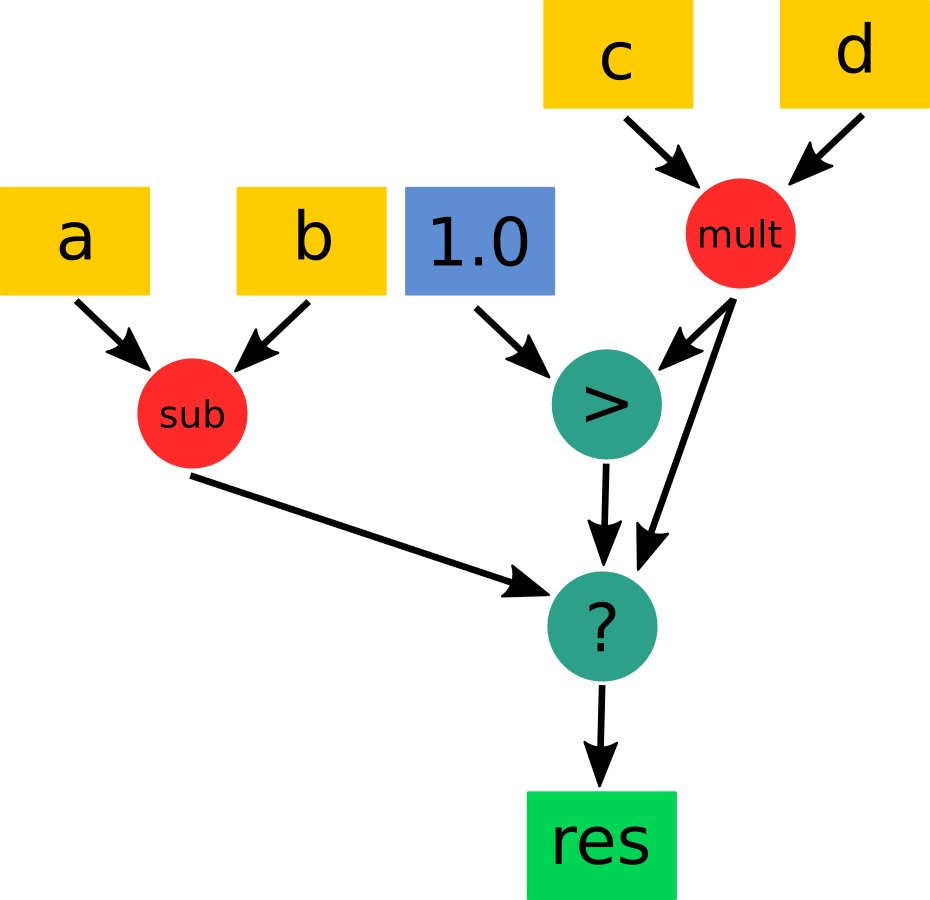
\includegraphics[height=16em]{drawings/implementation-compute-graph.png}
	\caption{Example Compute Graph.}
	\label{fig:implementation-compute-graph}
\end{figure}


\paragraph{Latency}
In order to compute the global stencil program latency, we are interested in the critical path latency of each individual stencil. Using the graph representation of the AST and a static mapping of each operation to the number of cycles it takes to perform a single operation, we can simply walk up the tree from the result and sum up the latency of each computation node till an input node is being reached. The highest latency value at some input corresponds to the overall critical path latency of the stencil.


\paragraph{Internal Buffer} \label{para:internal-buffer}
We refer to the internal buffer as the buffer space required such that each input data element has to be fetched or read only once. In other words, we want to store all data elements once they have been used for the first time by this specific stencil till they retire (not being required any longer) as shown in figure \ref{fig:model-internal-buffer}. \\
To get a good understanding, we derive the formula of this calculation by looking at some examples. Without loss of generality, we assume that we have a single three dimensional input data grid that we are looping over (figure \ref{fig:buffer-array}) using our stencil where the center element of the stencil is the field we are producing the result for. The derived formula can be extended to multiple different input arrays by splitting the field accesses for each input array and solve the problem for each of them. Furthermore, we iterate over the array in the following dimensional order:
\begin{minted}{python}
for i=1..Z
  for j=1..Y
    for k=1..X
\end{minted}


\begin{figure}[h]
	\begin{minipage}{.5\columnwidth}
	\centering
	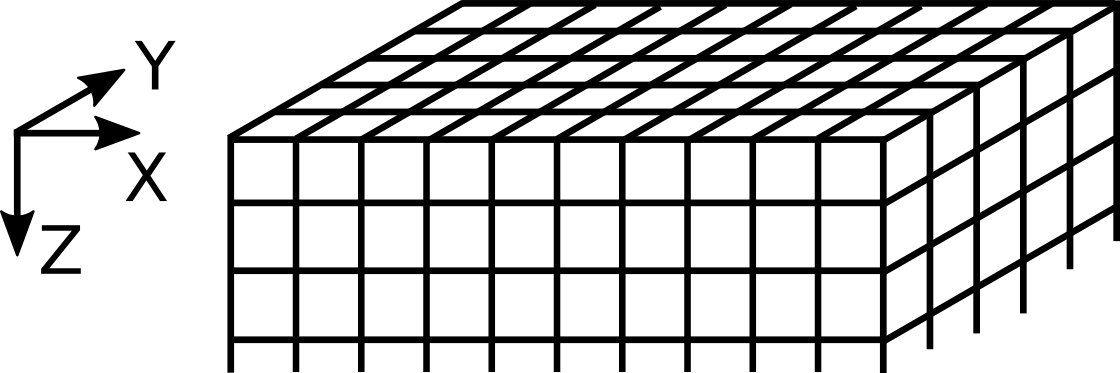
\includegraphics[height=5.5em]{drawings/buffer-array.png}
	\caption{Data array.}
	\label{fig:buffer-array}
	\vspace{-10.5em}
	\end{minipage}
	\begin{minipage}{.5\columnwidth}
	\centering
	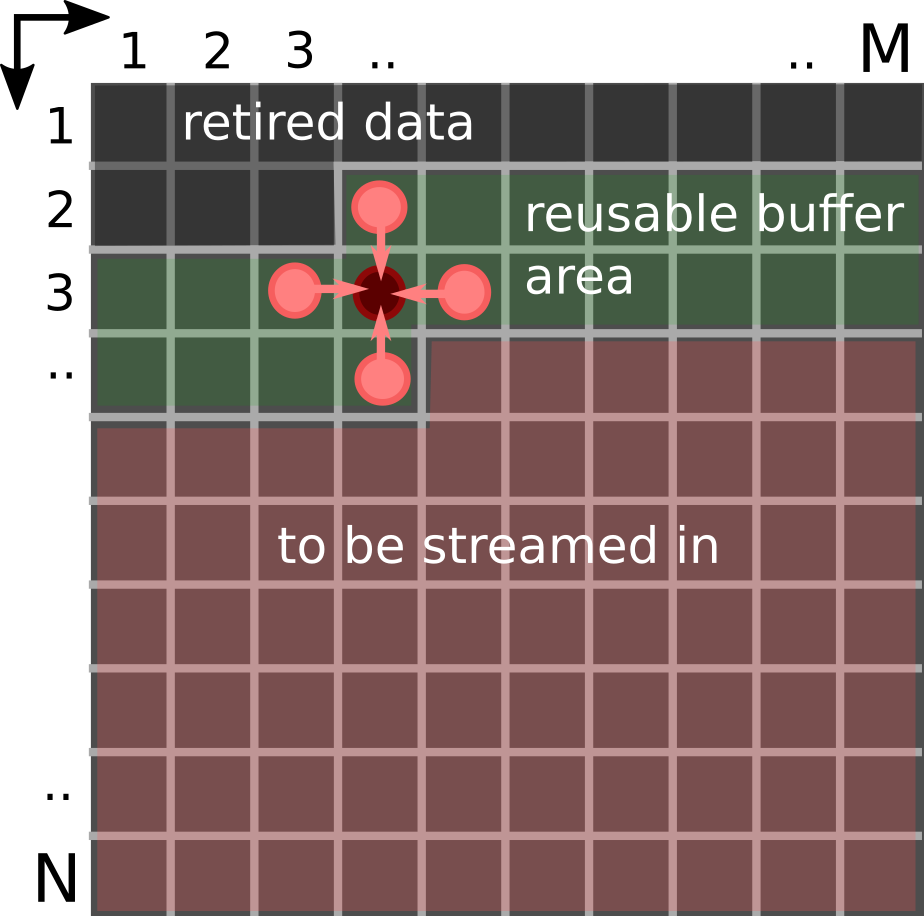
\includegraphics[height=16em]{drawings/model-internal-buffer.png}
	\caption{Internal Buffer of a Stencil.}
	\label{fig:model-internal-buffer}
	\end{minipage}
\end{figure}


\subparagraph{Example 1: Single Element}
Our first example is a kernel that simply multiplies the only input element by a factor of 7.0. Furthermore, the only field access is at the same location on the grid as we write the output to (at [i,j,k]). 
\begin{align}
\text{out}(i, j, k) = 7.0 \cdot \text{in}(i, j, k)
\end{align}
This leads to a stencil consisting only of a single element (namely the center element itself) as illustrated in figure \ref{fig:buffer-ex1-no-buffer}. \\
Figure \ref{fig:buffer-ex1-buffer} shows the internal buffer of such a stencil operator, which is one data element wide. As soon as the data element has been read, it will not be used anymore and it can therefore be discarded. \\
\begin{figure}[h]
	\begin{minipage}{.5\columnwidth}
		\centering
		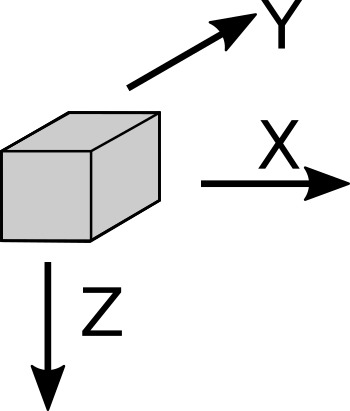
\includegraphics[height=12em]{drawings/buffer-ex1-no-buffer.png}
		\caption{Example 1: Stencil Operator.}
		\label{fig:buffer-ex1-no-buffer}
	\end{minipage}
	\begin{minipage}{.5\columnwidth}
		\centering
		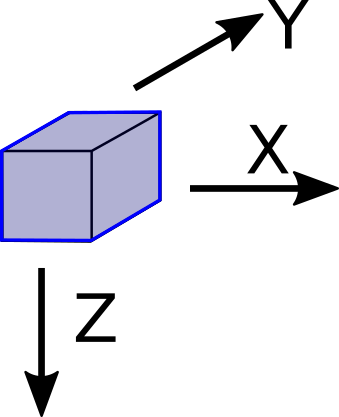
\includegraphics[height=12em]{drawings/buffer-ex1-buffer.png}
		\caption{Example 1: Internal Buffer laid over the Stencil.}
		\label{fig:buffer-ex1-buffer}
	\end{minipage}
\end{figure}

This number can also be derived by computing the difference between the highest and the lowest access index and adding one.
\begin{align}
\text{max index} - \text{min index} + 1 = [i, j, k] - [i, j, k] + 1 = [0, 0, 0] + 1
\end{align}
We will check with more complex examples if the formula also holds for them.\\


\subparagraph{Example 2: 1D Stencil}
Our second example consists of a stencil that sums over the center element and its predecessor and successor element in X direction. 
\begin{align}
\text{out}(i, j, k) = \text{in}(i, j, k-1) + \text{in}(i, j, k) + \text{in}(i, j, k+1)
\end{align}
Therefore, the stencil consists of three cubes (figure \ref{fig:buffer-ex2-no-buffer}) laid out next to each other in the direction of the X axis.\\
The internal buffer size of such a stencil operator is three data element wide. This can be verified by hand since we are in the innermost loop and the stencil therefore moves forward each iteration by one element in X direction. Therefore, the element read by the field access [i,j,k+1] can be discarded after the last stencil access ([i,j,k-1]) made use of it. 
\begin{figure}[h]
	\begin{minipage}{.5\columnwidth}
		\centering
		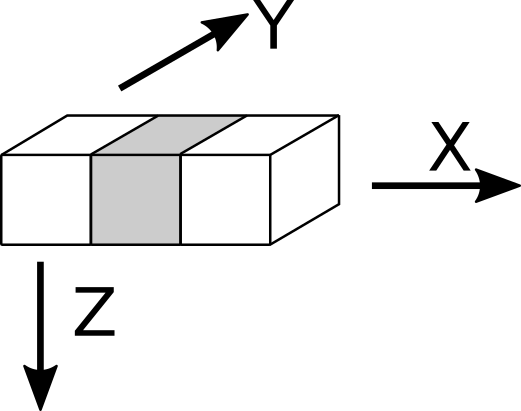
\includegraphics[width=0.7\textwidth]{drawings/buffer-ex2-no-buffer.png}
		\caption{Example 2: Stencil Operator.}
		\label{fig:buffer-ex2-no-buffer}
	\end{minipage}
	\begin{minipage}{.5\columnwidth}
		\centering
		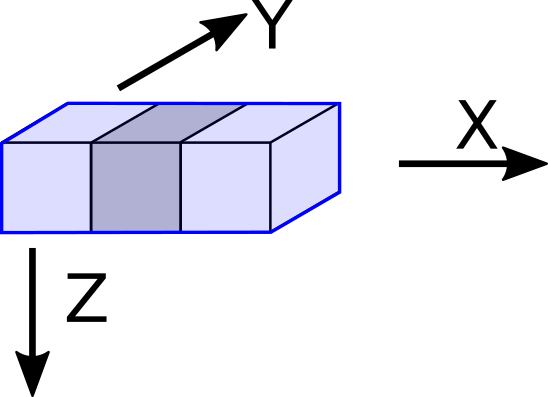
\includegraphics[width=0.7\textwidth]{drawings/buffer-ex2-buffer.png}
		\caption{Example 2: Internal Buffer laid over the Stencil.}
		\label{fig:buffer-ex2-buffer}
	\end{minipage}
\end{figure}


This number can also be derived by computing the difference between the highest and the lowest access index and adding one. 
\begin{align}
\text{max index} - \text{min index} + 1 = [i, j, k+1] - [i, j, k-1] + 1 = [0, 0, 2] + 1
\end{align}


\subparagraph{Example 3: 2D Stencil}
Our third example consists of a stencil that sums up its direct neighbors in the X-Y plane.
\begin{align}
\text{out}(i, j, k) = \text{in}(i, j, k) + \text{in}(i, j, k-1) + \text{in}(i, j, k+1) + \text{in}(i, j-1, k) + \text{in}(i, j+1, k)
\end{align}
Therefore, the stencil looks like a cross in the X-Y plane (figure \ref{fig:buffer-ex3-no-buffer}). \\
The internal buffer size of such a stencil is not a static number of elements anymore, but depends on the actual dimension sizes since the buffer is spread over a whole dimension. Using the graphic, you can verify that the buffer size of this specific stencil is 2*X + 1. 
\begin{figure}[h]
	\begin{minipage}{.5\columnwidth}
		\centering
		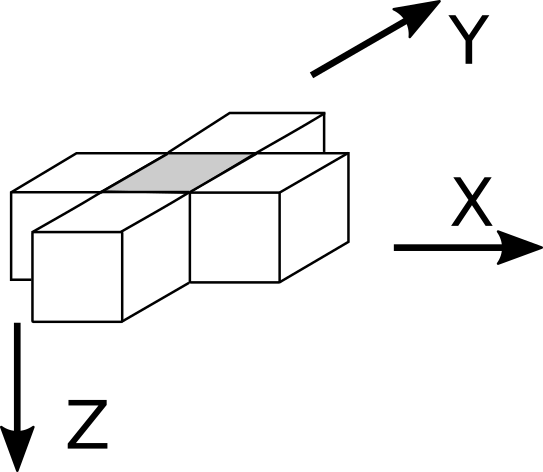
\includegraphics[width=0.7\textwidth]{drawings/buffer-ex3-no-buffer.png}
		\caption{Example 3: Stencil Operator.}
		\label{fig:buffer-ex3-no-buffer}
	\end{minipage}
	\begin{minipage}{.5\columnwidth}
		\centering
		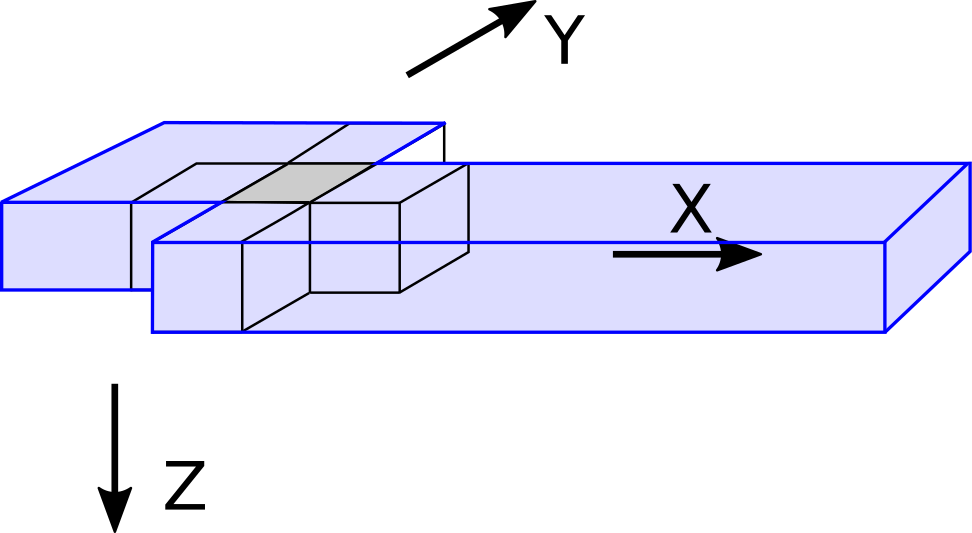
\includegraphics[width=1.0\textwidth]{drawings/buffer-ex3-buffer.png}
		\caption{Example 3: Internal Buffer laid over the Stencil.}
		\label{fig:buffer-ex3-buffer}
	\end{minipage}
\end{figure}


This number can also be derived by computing the difference between the highest and the lowest access index and adding one. 
\begin{align}
\text{max index} - \text{min index} + 1 = [i, j+1, k] - [i, j-1, k] + 1 = [0, 2, 0] + 1
\end{align}


\subparagraph{Example 4: 3D Stencil}
Our fourth example consists of a stencil that adds the center element with its neighbor in the Z dimension, which represents the outermost loop.
\begin{align}
\text{out}(i, j, k) = \text{in}(i, j, k) + \text{in}(i+1, j, k)
\end{align}
Therefore, the corresponding stencil looks like two cubes stacked above each other. \\
This time the buffer is even spread over two dimensions (i.e. layer of the X-Y plane. And has the size of X*Y + 1. 
\begin{figure}[h]
	\begin{minipage}{.5\columnwidth}
		\centering
		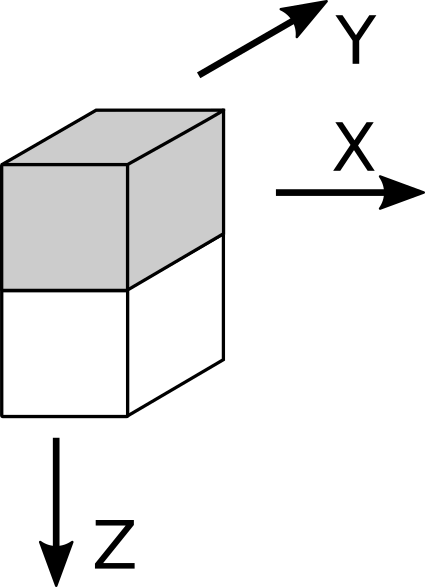
\includegraphics[width=0.5\textwidth]{drawings/buffer-ex4-no-buffer.png}
		\caption{Example 4: Stencil Operator.}
		\label{fig:buffer-ex4-no-buffer}
	\end{minipage}
	\begin{minipage}{.5\columnwidth}
		\centering
		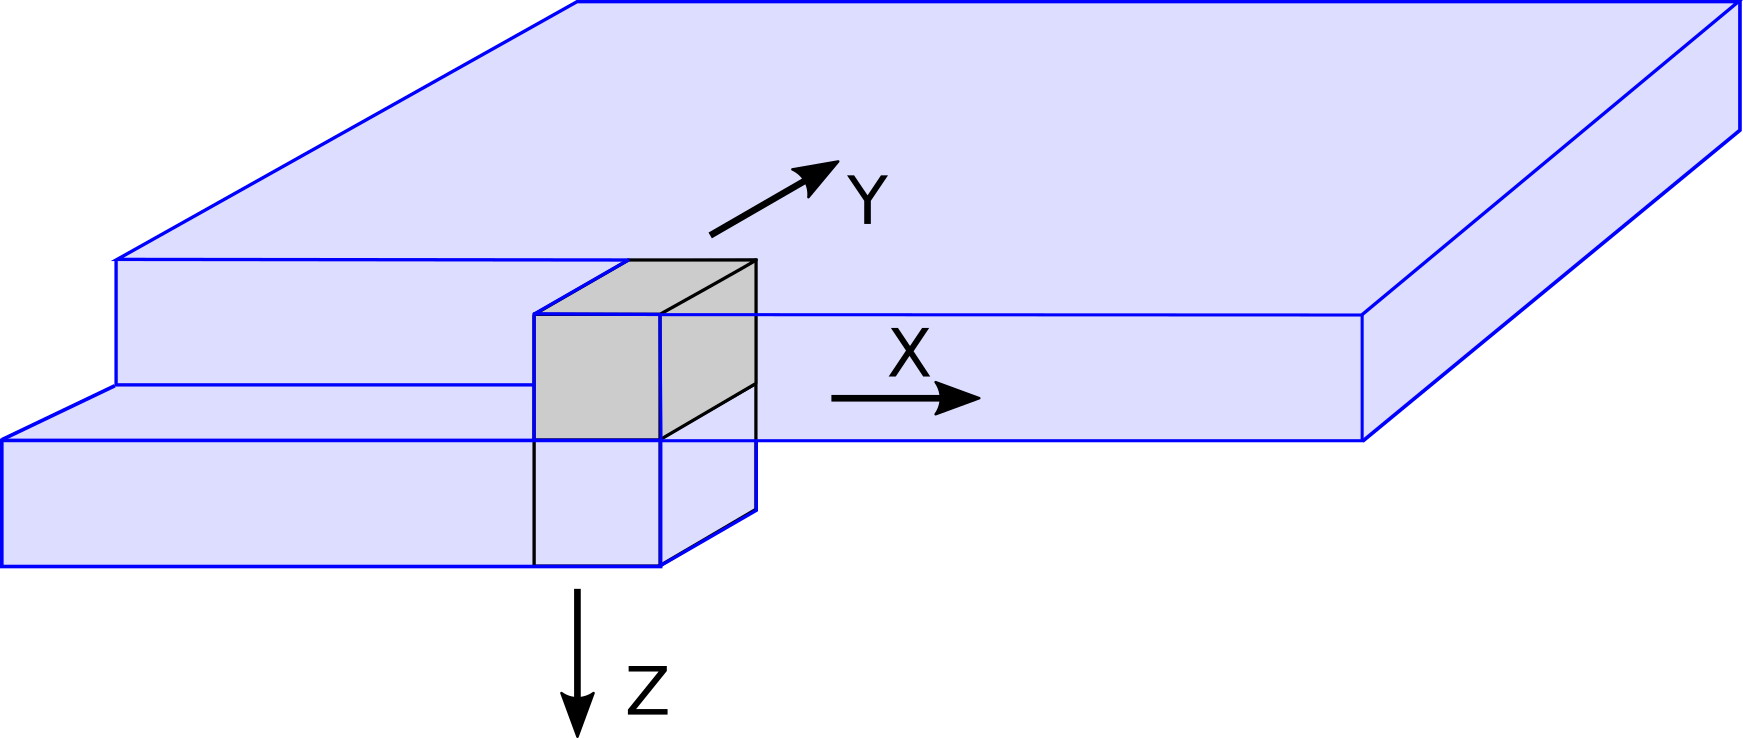
\includegraphics[width=1.0\textwidth]{drawings/buffer-ex4-buffer.png}
		\caption{Example 4: Internal Buffer laid over the Stencil.}
		\label{fig:buffer-ex4-buffer}
	\end{minipage}
\end{figure}

This number can also be derived by computing the difference between the highest and the lowest access index and adding one. 
\begin{align}
\text{max index} - \text{min index} + 1 = [i+1, j, k] - [i, j, k] + 1 = [1, 0, 0] + 1
\end{align}


\subparagraph{}
We can conclude that the internal buffer size can be computed in general using the following formula: \\
\begin{align}
\text{max index} - \text{min index} + 1
\end{align}


\subparagraph{Dimensional Notation} 
We refer to this notation of square brackets as the dimensional notation. This format is internally used in StencilFlow since it has the great benefit of being independent of the actual problem dimensions.  
The relation from the dimensional form to an absolute value is given by:
\begin{lstlisting}[showstringspaces=false, frame=single, language=Python]  
given: 
input dimensions [X,Y,Z]   
value in dimensional format: [a,b,c]
absolute size: x + X*b + X*Y*a = c + X*(b  + Y*a)
\end{lstlisting}



\subsection{Stencil Program}
The stencil program graph represents the highest level of abstraction of the stencil program. It is required to represent dependencies between different kernels and computes global properties combined from the individual stencils.


\paragraph{Stencil Program Graph}
The graph consists of input, kernel and output nodes. The input nodes represents the actual data array inputs, the kernel nodes represent stencil computations and the output nodes store the result of the computation. Edges between them are called channels and provide forwarding and buffer functionality for the pipeline. 
\begin{figure}[h]
	\centering
	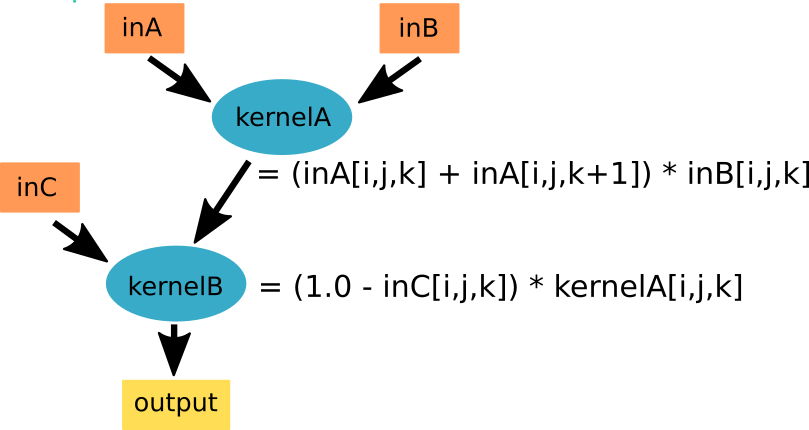
\includegraphics[height=16em]{drawings/approach-stencil-program.png}
	\caption{Example Kernel Chain Graph.}
	\label{fig:approach-stencil-program2}
\end{figure}


\paragraph{Latency}
The critical path latency of the stencil program graph is an important metric to compute the actual runtime of the program in hardware. Given the design frequency, the (theoretical) runtime is: $\frac{(critical\_path\_length + X*Y*Z)}{frequency}$. \\
The critical path computation is identical to the calculation for the compute graph. We can assign latency zero to the output nodes and walk up the tree to the inputs while adding the critical kernel latency computed by the ComputeGraph.



\paragraph{Delay Buffer}
We call the second type of buffering required to run a fully pipelined design delay buffer (beside the internal buffer described in the kernel section \ref{para:internal-buffer}). As the name suggest, its purpose is to latch intermediate data till the kernel is ready to read from the channel. This data dependency arises at the inter-kernel-level, which is why the stencil program graph has to take care of this. The following example illustrates a case where this is required.\\
The output of kernelA for kernelD is ready some time before the data stream from kernelC to kernelD arrives. Since kernelD cannot start processing the input data from kernelA, but rather has to wait for the data from kernelC, we have to introduce a delay buffer at the edge from A to D. The size of this delay buffer is (assuming field accesses of D from C and A are identical e.g kernelD[i,j,k] = kernelA[i,j,k] + kernelC[i,j,k]) given by the latency of the path kernelA-kernelB-kernelC-kernelD.   
\begin{figure}[h]
	\begin{minipage}{.5\columnwidth}
		\centering
		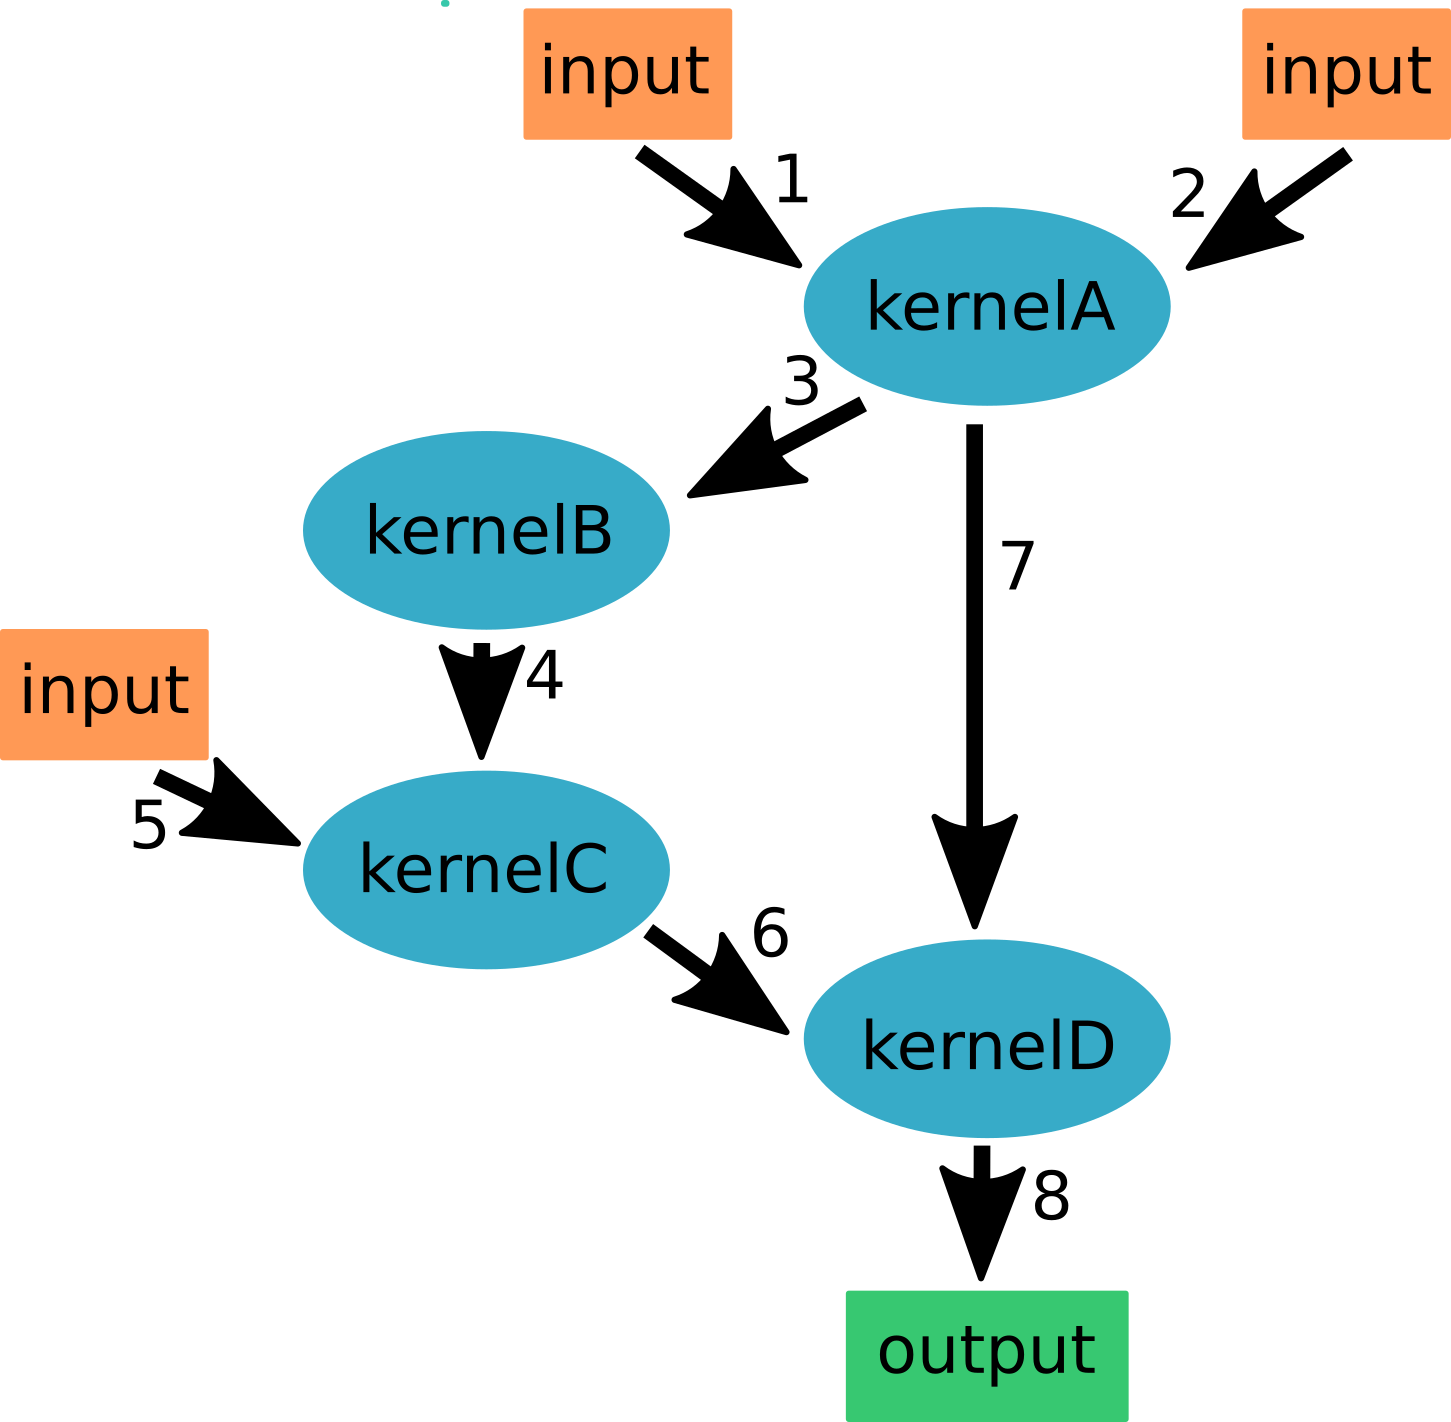
\includegraphics[height=16em]{drawings/model-delay-buffer1.png}
		\caption{Example stencil program.}
		\label{fig:model-delay-buffer}
		\vspace{1em}
	\end{minipage}
	\begin{minipage}{.5\columnwidth}
		\centering
		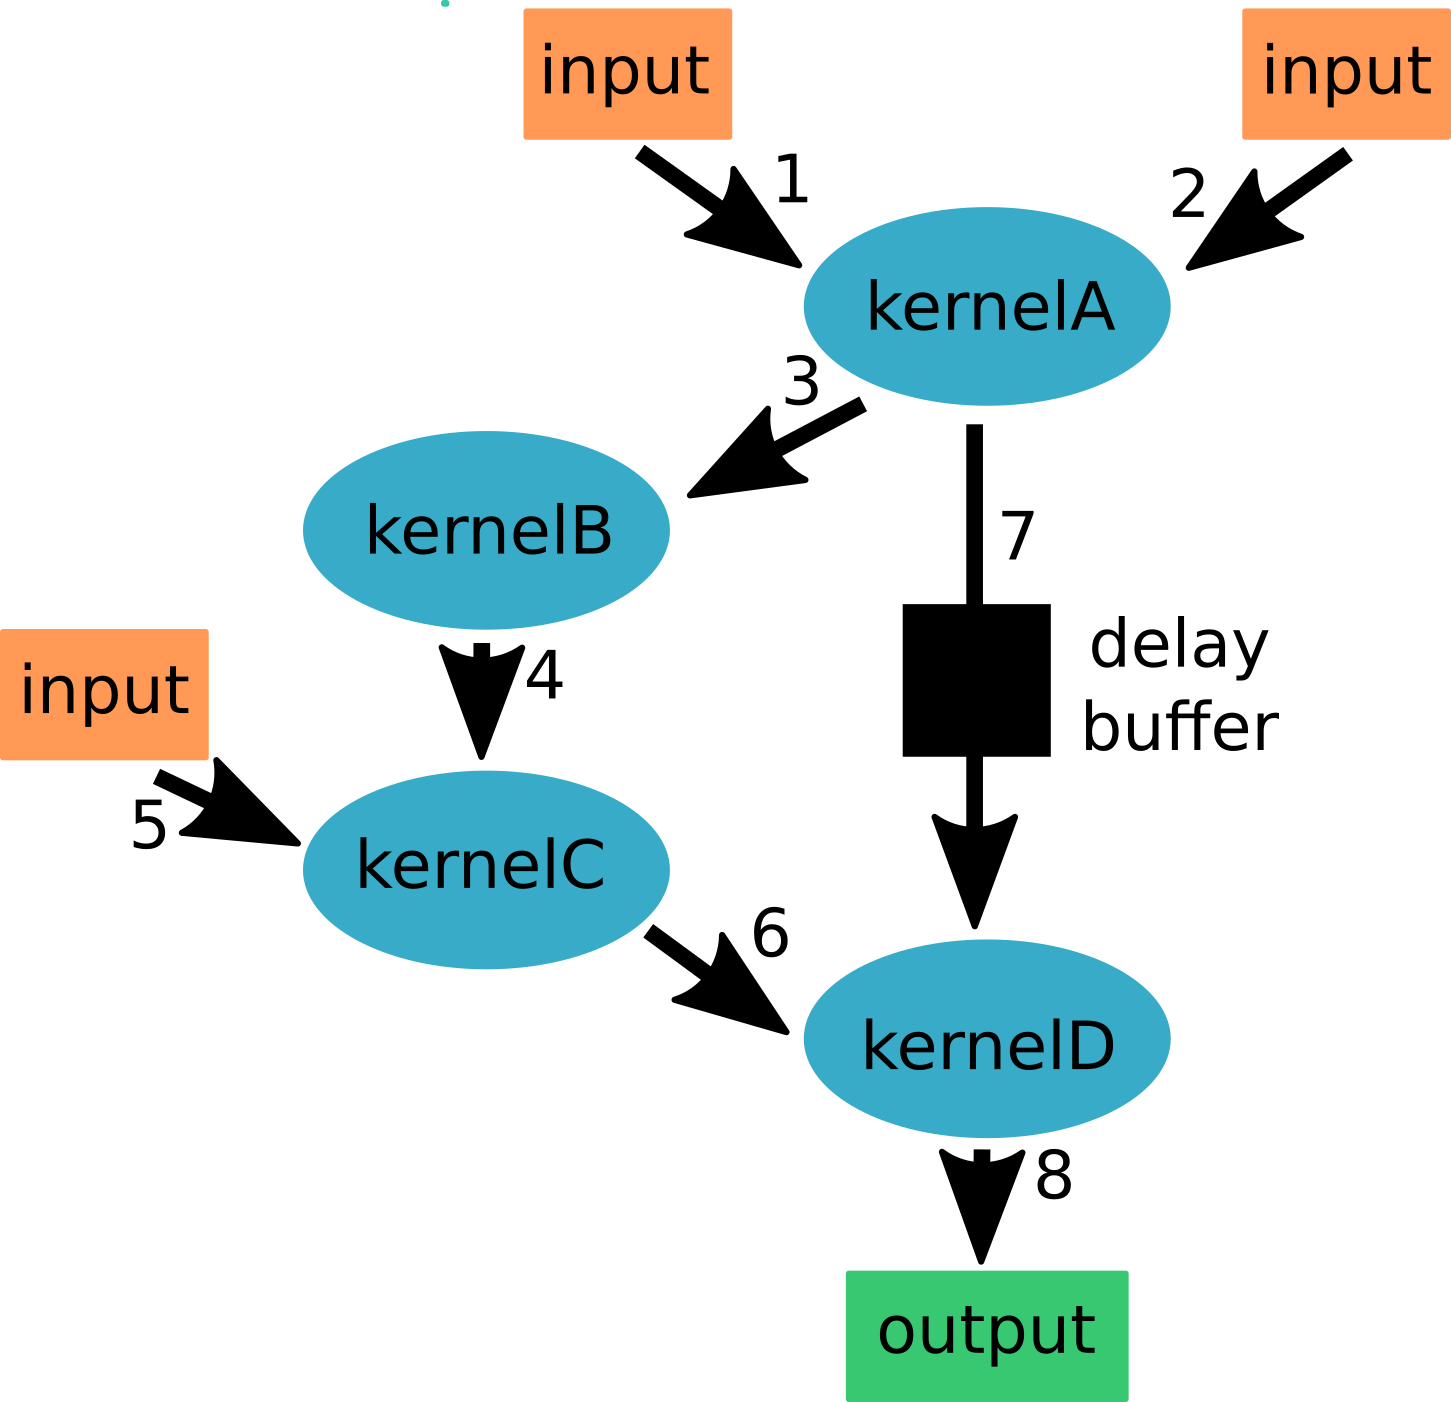
\includegraphics[height=16em]{drawings/model-delay-buffer2.png}
		\caption{Example stencil program with delay buffer.}
		\label{fig:model-delay-buffer2}
	\end{minipage}
\end{figure}



\section{FPGA Model}
Since we are dealing with a memory bound problem and seek to optimize for maximal throughput, our model is very data-centric, especially since todays state-of-the-art FPGAs offer such a huge amount of hardened digital signal processors (DSPs) (e.g. 10 TFLOP/s peak 32-bit floating point operations on a Stratix 10 \label{label25}). Therefore we assume that we are limited by either on-chip memory capacity or off-chip memory bandwidth.
\begin{figure}[h]
	\centering
	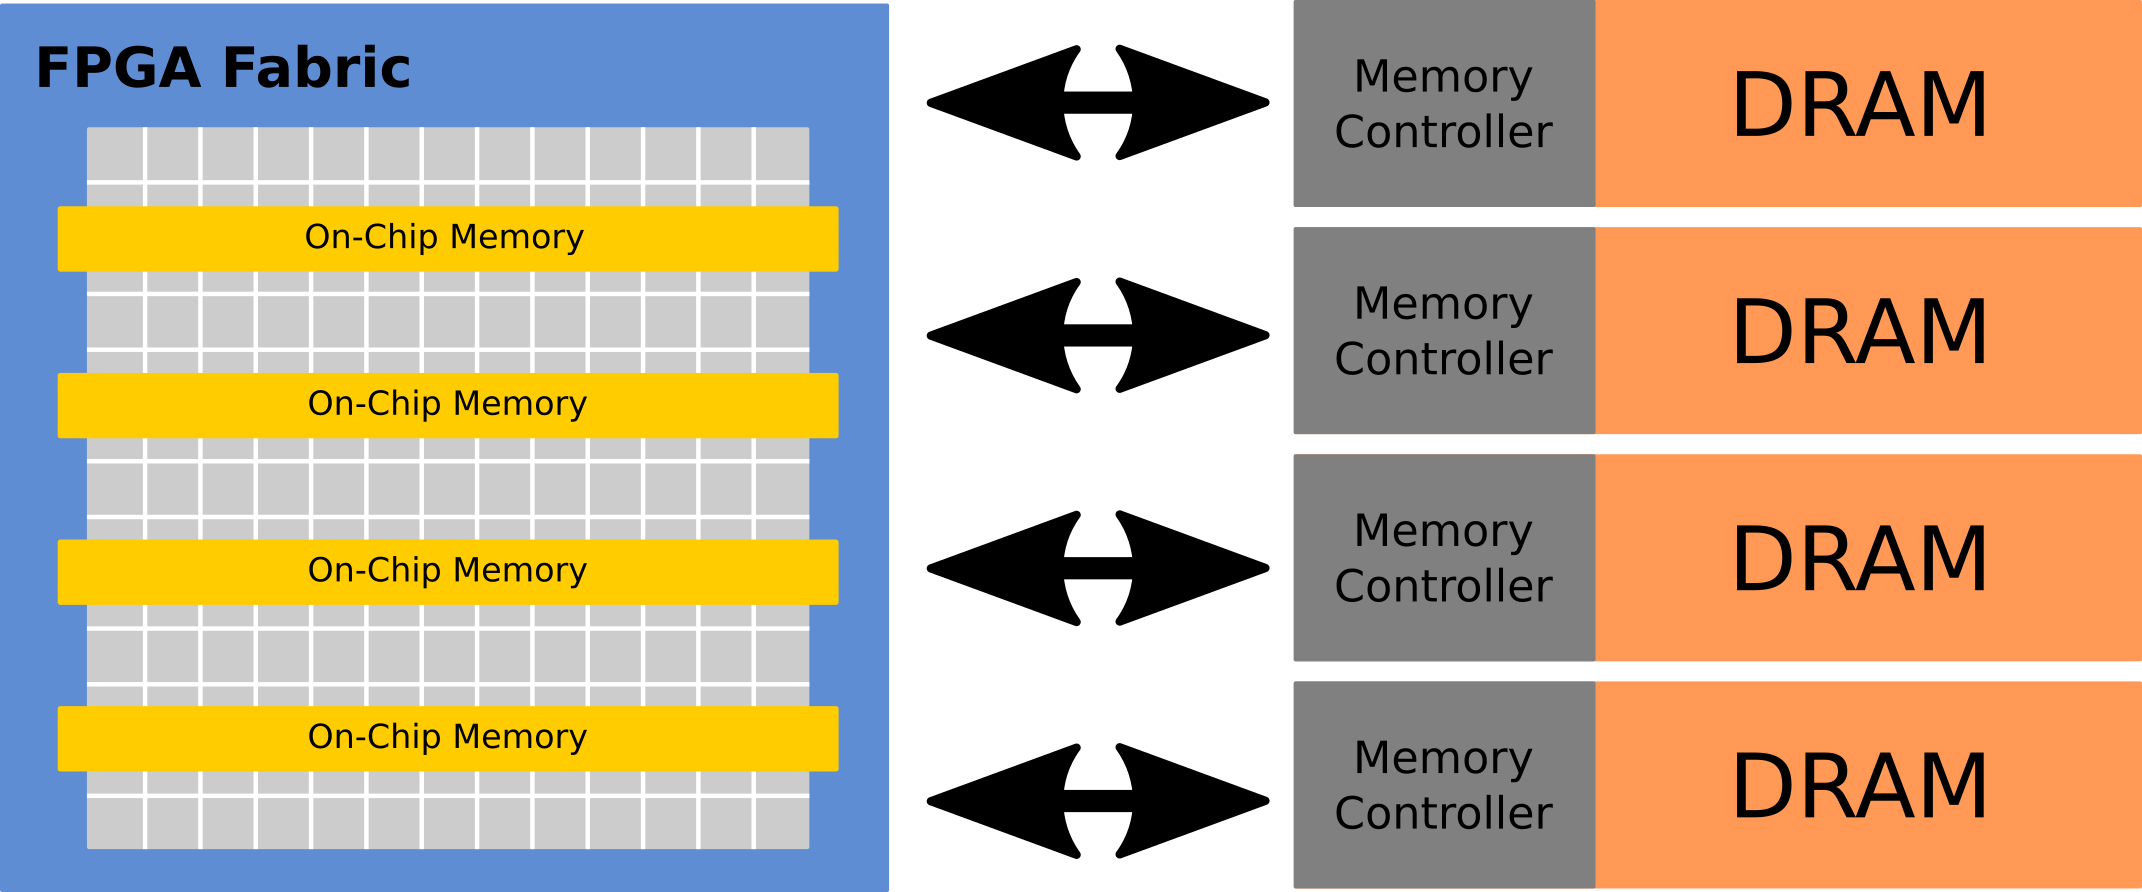
\includegraphics[height=12em]{drawings/optimizer-memory-system.png}
	\caption{Basic memory model: Fast on-chip memory, slow DRAM memory and memory bandwidth.}
	\label{fig:optimizer-memory-system}
\end{figure}


\subsection{Fast and Slow Memory}
Since we fully pipeline the whole stencil program, we need to lay out all the internal and delay buffers in memory. While the fast on-chip memory of the FPGA has very low latency/high throughput and a low energy footprint compared to the slow DRAM memory (including the data path to the DRAM), it is a limited resource and we have to carefully choose which buffers we allocate in fast memory and which we better swap out to the slow memory.


\subsection{Memory Bandwidth}
Furthermore, even before having filled up the whole DRAM with buffers, we might run into the issue that we run out of bandwidth between the DRAM and the FPGA fabric. Therefore, memory bandwidth is a key metric too, which we have to take into account in the optimization process.




\section{Hardware Mapping: DaCe}
Despite our high-level optimization, it has been shown that FPGA designs can gain significant performance increase \cite{label57} if the HLS design has been further optimized and equipped with the suitable pragmas and formulations. \\
Therefore, we decided to decouple the high-level representation from the lower-level and use DaCe \footnote{https://github.com/spcl/dace}, which is able to compile FPGA code with high utilization and performance from the intermediate representation, the so called Stateful DataFlow multiGraph (SDFG) \cite{label57}. \\
The SDFG intermediate representation is a directed graph of directed acyclic multi graphs, where the nodes represent computations and storage while the edges represent data movement. Figure \ref{fig:dace-sdft-syntax} summaries all graph primitives of the stateful dataflow multigraph. \\ 
\begin{figure}[h]
	\centering
	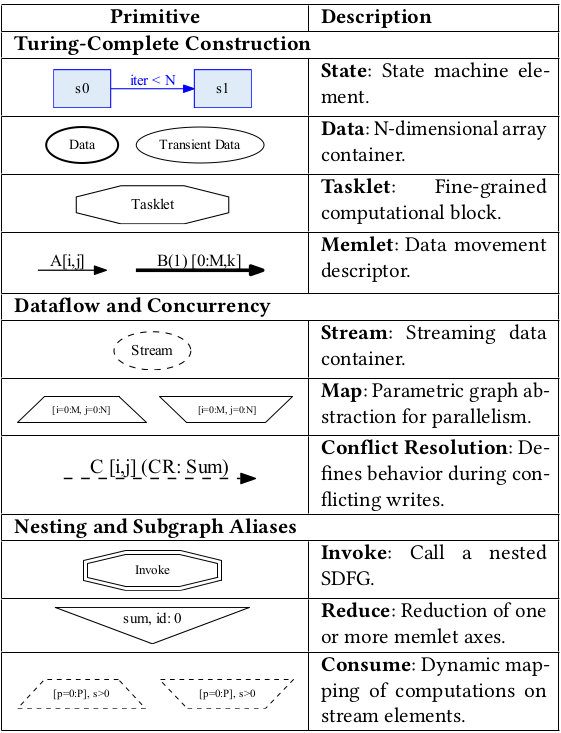
\includegraphics[height=16em]{images/dace-sdft-syntax.png}
	\caption{SDFG primitives syntax and description. \cite{label57}}
	\label{fig:dace-sdft-syntax}
\end{figure}

In order to get a better understanding we look at the transformation of vector addition from python code to the SDFG graph representation. 
\begin{minted}{python}
def vector_add(A, B):
  return list(map(lambda x,y: x+y, A, B))
\end{minted}
The corresponding graph starts with the two N-dimensional array containers A and B, which are connected by a data movement descriptor (memlet) through a map with the fine-grained computational block (tasklet). The map primitive splits the N-dimensional problem into N parallel 1-dimensional sub-problems in order to exploit the implicit parallelism. This is illustrated in figure \ref{fig:dace-vetor-add-n3} for the case N=3. The tasklet describes this element-wise computation:
\begin{align}
\text{C}[i] = \text{A}[i] + \text{B}[i]
\end{align}
The resulting is then mapped back to the N-dimensional form and finally stored in the output data container C as shown in figure \ref{fig:dace-vector-add}.
\begin{figure}[H]
	\begin{minipage}{.5\columnwidth}
		\centering
		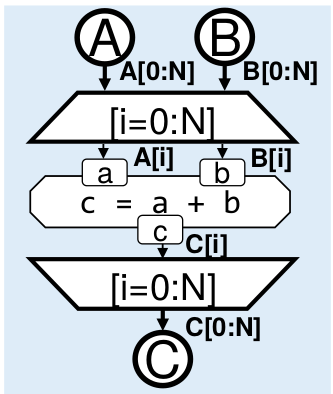
\includegraphics[height=12em]{images/dace-vector-add.png}
		\caption{SDFG in parametric form. \cite{label57}}
		\label{fig:dace-vector-add}
		\vspace{1.5em}
	\end{minipage}
	\begin{minipage}{.5\columnwidth}
		\centering
		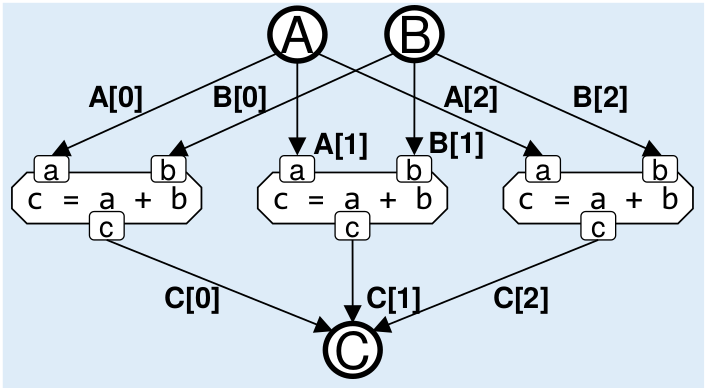
\includegraphics[height=12em]{images/dace-vetor-add-n3.png}
		\caption{SDFG expanded for N=3. \cite{label57}}
		\label{fig:dace-vetor-add-n3}
	\end{minipage}
\end{figure}

This general graph representation builds the foundation for the transformation and optimization to different hardware platforms, which makes DaCe a very powerful toolbox. It incorporates many optimization techniques such as tiling and fusion in order to generate efficient code for the specific platform. Figure \ref{fig:dace} shows the complete transformation process form the domain specific high-level program to the hardware-specific optimized design.
\begin{figure}[h]
	\centering
	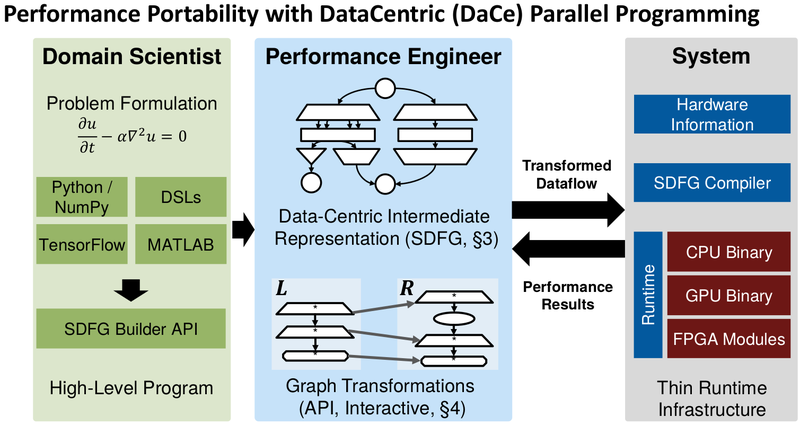
\includegraphics[width=1.0\textwidth]{images/dace.png}
	\caption{ \textit{Presentation Slide: Data-Centric Parallel Programming,Torsten Hoefler, invited talk at ISC’19, Frankfurt, Germany}}
	\label{fig:dace}
\end{figure}




\section{Conclusion}
So far, we have seen that the actual problem to solve is trading the different compromise in resource allocation against each other to find a feasible and well performing design. The foundation for such an optimization has been laid down in this chapter by formalizing the analysis of resource requirements. In the next chapter, we will have a look on how we can formalize a objective and find the (theoretical) optimal solution within our specific assumptions.












 % done
\chapter{Optimizer}
The aim of mathematically modeling stencil programs for reconfigurable hardware is to have a formal way of arguing about the optimal and efficient usage of the available resources. This section is dedicated to explaining what we are optimizing for and how we are achieving a maximized objective.


\section{Objective}
In stencil programs, each compute operation usually depends on multiple data field accesses which makes them very memory heavy applications. The re-programmable nature of FPGAs allows us to make use of the fine grained access to fast on-chip memory in order to speed up or shorten the data path a data element has to take from its storage location to the actual compute unit. The objective we seek to achieve is to make optimal use of the very limited resource of fast memory, in conjunction with the available memory bandwidth and slow memory. By caching resources for re-use and exploitation of the efficient pipelining nature of modern FPGAs we try to get a fully pipelined design with a minimal amount of pipeline stalls due to waiting for data to arrive. \\
We mathematically formalize the problem by formulating it as an linear program.

$
\text{Objective 1: minimize fast memory usage:} \min\limits_{(X,Y)} F(X,Y)
\\
\text{Objective 2: minimize communication volume:} \min\limits_{(X,Y)} COM(X,Y)
\\
\text{Objective 3: optimize for ratio:} \min\limits_{(X,Y)} (\text{RATIO} - \frac{F(X,Y)}{COM(X,Y)})
\\
\\
\text{subject to:}
\\
\\
F(X,Y) = \sum_{(i,j)}D(X_{ij})*(1-X_{ij}) + \sum_{(i,j)}D(Y_{ij})*(1-Y_{ij}) \leq \text{ FAST\_MEMORY\_BOUND}
\\
\\
S(X,Y) = \sum_{(i,j)}D(X_{ij})*X_{ij} + \sum_{(i,j)}D(Y_{ij})*Y_{ij} \leq \text{ SLOW\_MEMORY\_BOUND}
\\
\\
C(X,Y) = \sum_{(i,j)}\text{comm\_vol}(X_{ij}) + \sum_{(i,j)}\text{comm\_vol}(Y_{ij}) \leq \\ \text{ COMMUNICATION\_VOLUME\_BOUND}
\\
\\
\\
\text{where the variables are denoted as:}
\\
\\
X_{ij}=
\begin{cases}
1, & \text{if j-th part of the internal buffer of kernel i allocated in slow memory}\\
0, & \text{otherwise}
\end{cases}
\\
\\
Y_{ij}=
\begin{cases}
1, & \text{if the delay buffer between kernel i and j is allocated in slow memory}\\
0, & \text{otherwise}
\end{cases}
\\
\\
\forall X_{ij}: D(X_{ij}) = \text{size of j-th part of the internal buffer of kernel i}
\\
\\
\forall Y_{ij}: D(Y_{ij}) = \text{size of the delay buffer between kernel i and j}
$
\\
\\
In the next section we will show the optimization approach to achieve this goal and further explain how the function comm\_vol is derived.  
\begin{figure}[h]
	\centering
	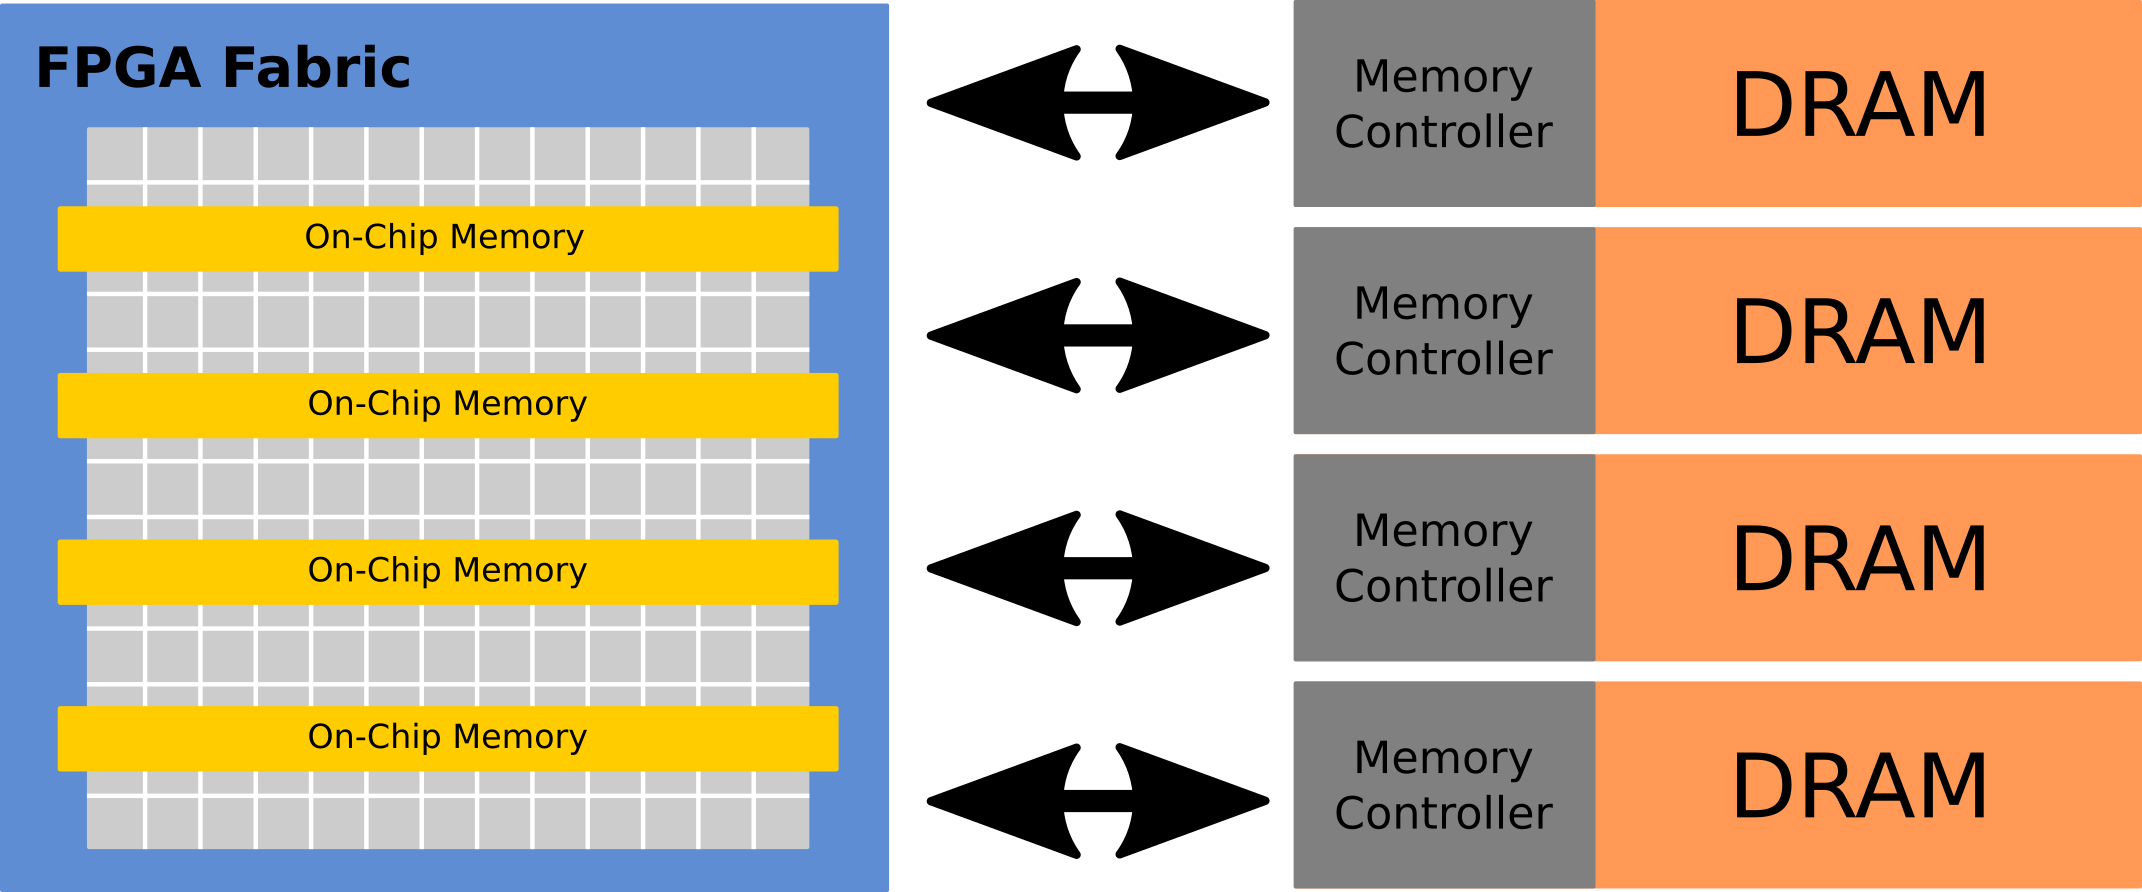
\includegraphics[height=12em]{drawings/optimizer-memory-system.png}
	\caption{High level overview of the abstracted FPGA with the key resources: fast/slow memory and memory bandwidth.}
	\label{fig:optimizer-memory-system2}
\end{figure}

\section{Approach}
We start our algorithm by putting all buffers (internal and delay) into fast memory. Then, we swap out the buffer that uses the memory \textit{most inefficiently} to slow memory. We repeat this till we reach the goal of the strategy chosen. We will walk through an example to get an intuition of the decision for the right choice of swapping out.


\paragraph{Most Inefficient Buffer}
We move the buffer with the highest metric \\ $\frac{\textrm{memory size(buffer)}}{\textrm{communication volume(buffer)}}$) from fast to slow memory. In other words, we "pay" communication volume and slow memory (we do not bother about the slow memory, since this is usually orders of magnitudes larger than the fast memory) for getting rid of some amount of buffer space. The buffer with the highest metric value get is optimal to swap out, since we "pay" the least amount compared to the size of the buffer we can remove from fast memory. \\
Since the communication volume of a buffer depends on the predecessor and successors location in memory, we will walk through an example to derive the rule for calculating the actual value. 


\subparagraph{Initial state}
In figure \ref{fig:optimizer-all-fast-memory} you can see the channel from the input kernel to the next kernel, split up into the delay buffer and the junks of the internal buffer (each part is from one field access to the next). For example a kernel \textit{out[i] = in[i-2] + in[i] + in[i+10]} would have one delay buffer and the internal buffer split into two parts of size 2 and 10. At the moment, they are all allocated in fast memory. We will analyze the communication volume for the darker part of the internal buffer dependent on the location of its predecessor and successor. \\
We can observe that the communication volume imposed by our buffer is zero if the predecessor and successor are in located in fast memory too. 



\subparagraph{Swap Out of Marked Buffer}
We moved out the marked buffer to slow memory (figure \ref{fig:optimizer-main-slow-memory}), which imposes an additional communication volume of $2*X*Y*Z$ 

\begin{figure}[h]
	\begin{minipage}{.5\columnwidth}
		\centering
		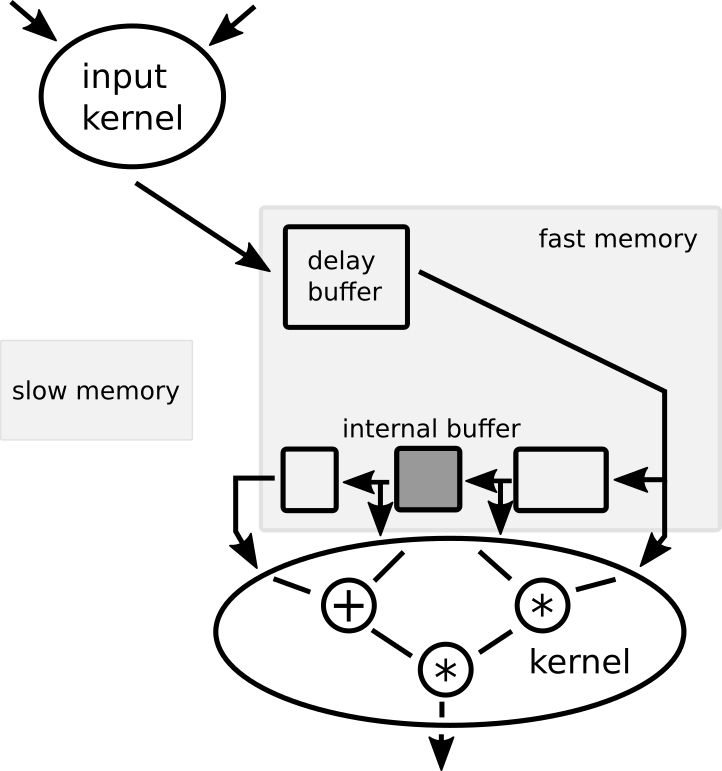
\includegraphics[height=16em]{drawings/optimizer-all-fast-memory.png}
		\caption{Scenario 1: All buffers are allocated in fast memory.}
		\label{fig:optimizer-all-fast-memory}
	\end{minipage}
	\begin{minipage}{.5\columnwidth}
		\centering
		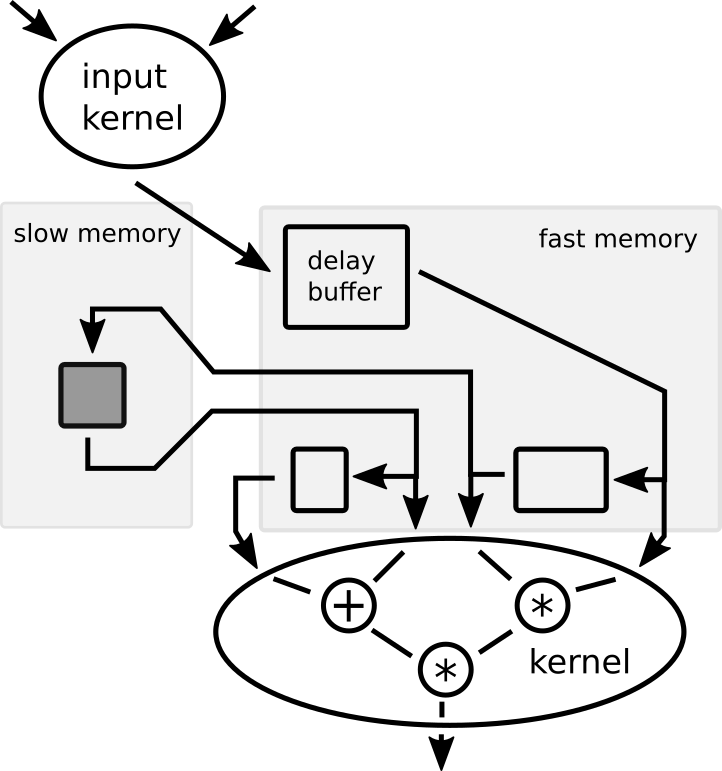
\includegraphics[height=16em]{drawings/optimizer-main-slow-memory.png}
		\caption{Scenario 2: The marked internal buffer is in slow memory but its predecessor and successor are in fast memory.}
		\label{fig:optimizer-main-slow-memory}
	\end{minipage}
\end{figure}

\subparagraph{Swap Out Successor}
This time, the successor of the marked buffer was already allocated in slow memory while the predecessor is still allocated in fast memory as shown in figure \ref{fig:optimizer-main-succ-slow-memory}. Moving out the marked buffer to slow memory imposes an additional communication volume of $1*X*Y*Z$. 


\subparagraph{Swap Out Predecessor and Successor}
Figure \ref{fig:optimizer-prev-main-succ-slow-memory} shows a situation where the predecessor and the successor have both already been swapped out. Swapping out the marked buffer in this situation actually does not impose any additional communication volume. The only thing changing is the direction of data movement (The output of the marked buffer was going from fast to slow, and now it goes into opposite direction)  
\begin{figure}[h]
	\begin{minipage}{.5\columnwidth}
		\centering
		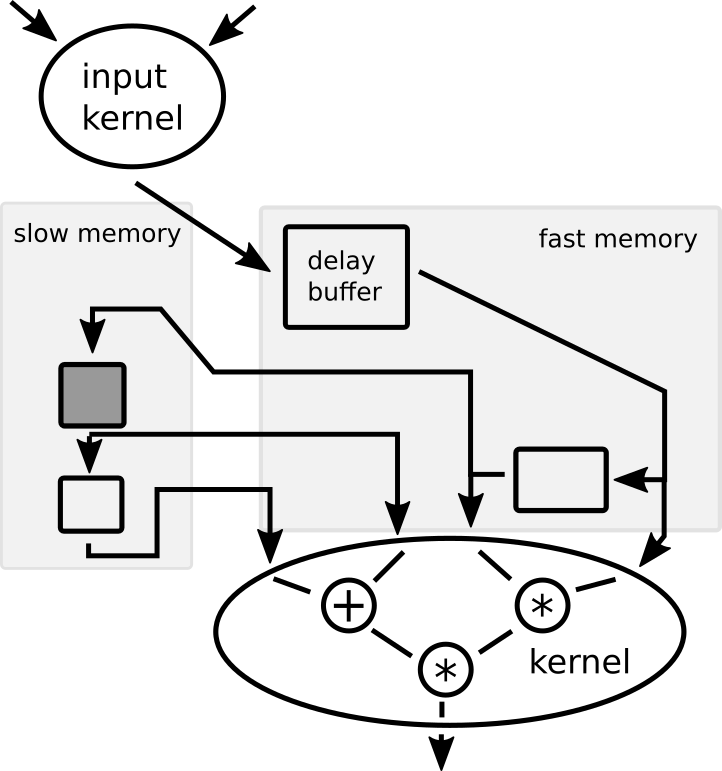
\includegraphics[height=16em]{drawings/optimizer-main-succ-slow-memory.png}
		\caption{Scenario 3: The marked internal buffer is in slow memory with its successor. The predecessor is allocated in fast memory.}
		\label{fig:optimizer-main-succ-slow-memory}
	\end{minipage}
	\begin{minipage}{.5\columnwidth}
		\centering
		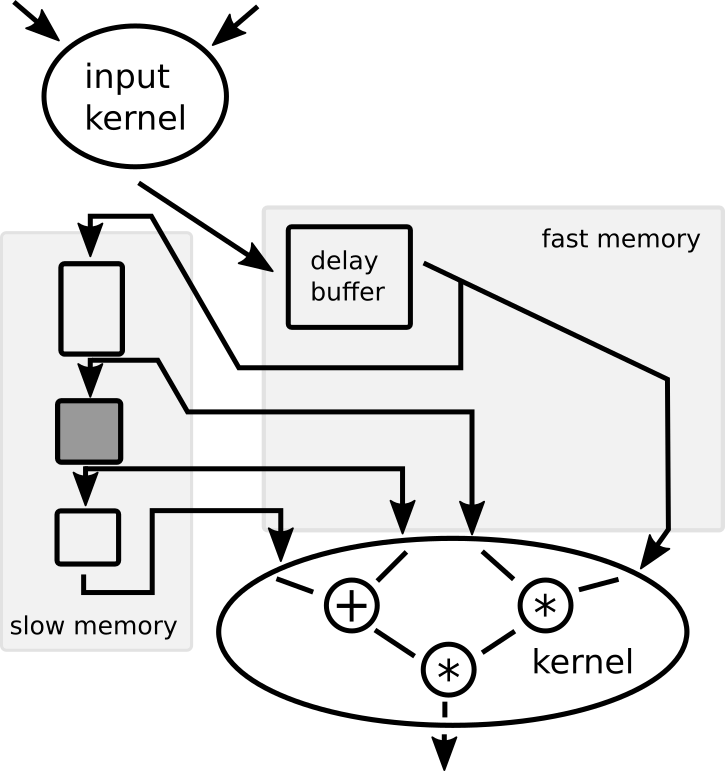
\includegraphics[height=16em]{drawings/optimizer-prev-main-succ-slow-memory.png}
		\caption{Scenario 4: The marked internal buffer is in slow memory together with its predecessor and successor.}
		\label{fig:optimizer-prev-main-succ-slow-memory}
	\end{minipage}
\end{figure}


\subparagraph{Conclusion}
The general rule for swapping the buffer out as explained in the previous example is given by: 
pre=predecessor
suc=successor
global array size = X*Y*Z = C
\begin{itemize}
	\item pred and succ in fast mem: 2*C
	\item pred in fast, succ in slow mem: C
	\item pred in slow, succ in fast mem: C
	\item pred and succ in slow mem: 0
\end{itemize}

\subparagraph{Optimizer}
On a high level, the optimizer works as follow:
\begin{algorithm}
	\caption{Optimizer}
	\begin{algorithmic}
		\WHILE{objective\_not\_reached}
		\STATE find buffer with highest metric value
		\STATE swap the buffer out
		\STATE update communication volume metric values for 
		\STATE its neighbors 
		\ENDWHILE
	\end{algorithmic}
\end{algorithm}


\section{Strategies}
Even though we have a fixed objective and a clear understanding on how we optimize, there are several scenarios with different requirements we can optimize for. 


\subparagraph{Minimization of Communication Volume}
Reduction of communication volume implies maximal usage of the fast on-chip memory resources and reduces data movement which is a natural choice of optimization.


\subparagraph{Minimization of Fast Memory}
Minimization of fast memory is a favorable strategy for example if one wants to use the remaining fast memory for other purposes. One such scenario would be tiling. 


\subparagraph{Optimization to Ratio}
This optimization strategy tries to optimize the buffer allocations in the best way to fit the ratio $\frac{\textrm{fast memory}}{\textrm{communication volume}}$ while staying below the upper bound of communication volume. This is a very useful metric if we assume that the DRAM (slow memory) is not our limiting factor and want to find out how many devices are required to fit the whole design onto it. If we choose the ratio of $\frac{\textrm{fast memory}}{\textrm{communication volume}}$ for a particular hardware device, we can reason about the number of devices required to implement our design as: $\textrm{number of required devices} = \frac{\textrm{fast memory size after optimization}}{\textrm{fast memory on a single device}}$
 % done
\chapter{Simulator}

We will go through a few arguments to underline that this is a good investment for time saving of future development.


\subparagraph{Debugging / Design Test}
Everybody that has already run FPGA designs in hardware knows that it is really hard to properly debug them in case of errors happening (e.g. deadlocks, etc.), since there is no notion of setting a breakpoint and look at the intermediate values as we are used to do this in software. What you can do is setting up a debug channel, which enables you to see at least what is happening on the device or where it breaks, but the capabilities remain very limited. \\
That's why we want the functionality to simulate the design in software first in order to eliminate as many bugs as possible. In case of problems, we can detect and debug them in the integrated development environment which gives us access to the current state of the whole design. This significantly reduces the error rate and increases the certainty of running on the actual hardware without issues.


\subparagraph{Correctness}
Furthermore, changes in the code generator, which will often occur in the future while doing the low-level performance optimization, might result in a working design, that produces invalid output data. Running the same input data on the simulator and compare the computation result to the one from the hardware gives us the opportunity to check the correctness of the hardware design without having to write a  dedicated golden model implementation for every problem.


\subparagraph{Performance Metrics}
Running the design in software gives us the benefit of being able to collect whatsoever information or metric we are interested in. This means that we cannot only test the design for correctness, but we can for example find out if the buffer size estimate is tight, in other words, that is the size exact and not just large enough.


\section{FPGA Execution Model}
The software execution model of the abstracted FPGA device is modular built up and transitions multiple phases, which we will have a look at now.


\subsection{Initialization}
In the initialization phase, we set up and load all input data into their corresponding allocated location. This is similar to the transfer of the input data from the host memory to the reconfigurable device.


\subsection{Step Execution}
After initialization we can start with the actual execution process. A single run of the so called step execution represents a clock cycle on the actual hardware. This is repeated till the stop condition is met, which will end the execution and initiates the transition over to the finalization process.  
\begin{figure}[h]
	\centering
	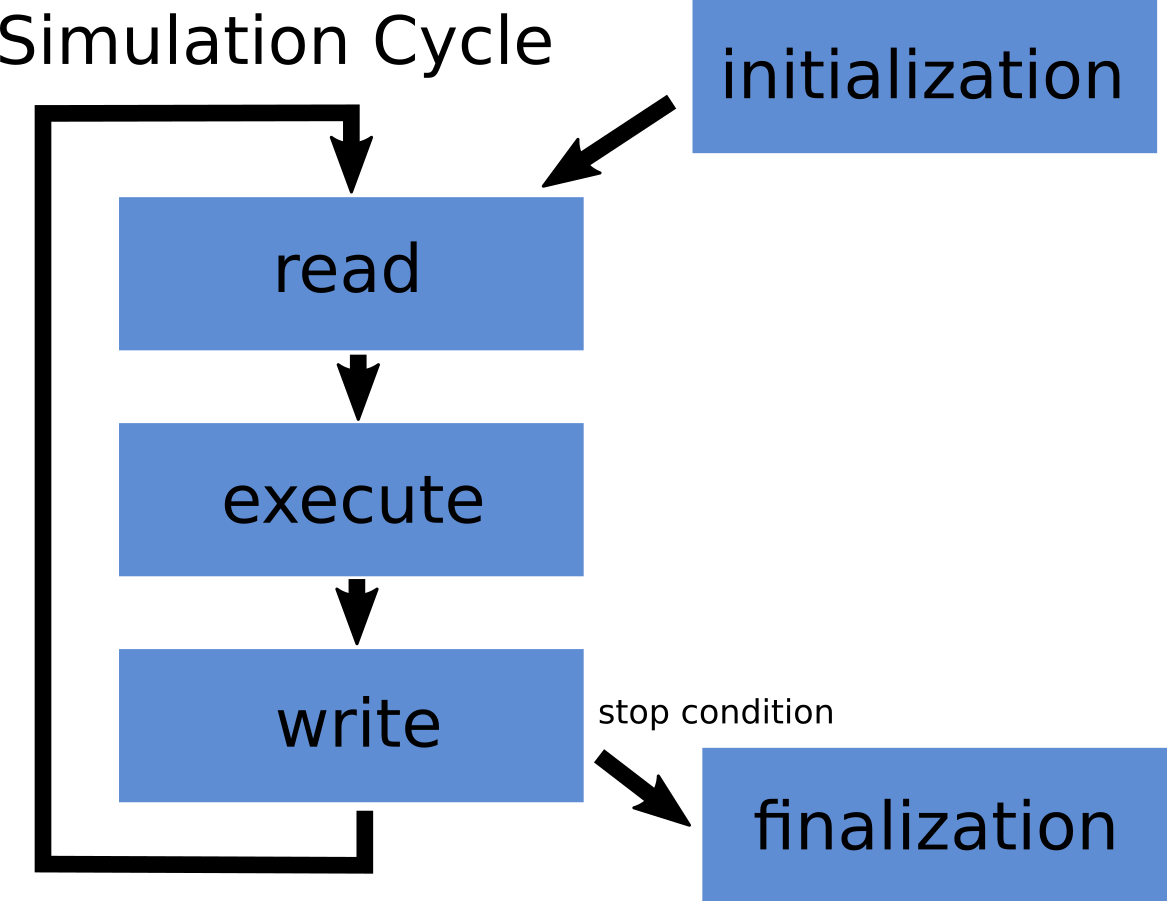
\includegraphics[height=12em]{drawings/simulator-simulation-cycle.png}
	\caption{Simulation Cycle: Step by step execution.}
	\label{fig:simulator-simulation-cycle}
\end{figure}


\subparagraph{Read}
In the read phase, all kernels check if data is available from all input channels. If this is the case they can consume them.


\subparagraph{Execute}
In the execution phase, all kernels that have successfully read data elements from all input channels can compute the output value according to the kernel function. In order to account for the operation latencies, the result is not directly written to the output channel, but rather hold back for \textit{latency} cycles.


\subparagraph{Write}
In the write phase, all kernels with valid output data write the result to the output channels, which are either input channels of other kernels or the channel collecting the final result for the transfer back to the host memory.


\subparagraph{Stop Condition}
The problem size respectively the number of data elements to process is given in the problem definition. Therefore we know after every kernel has written that many elements to the output channels, we can safely switch to the finalization phase.


\subparagraph{Finalization}
The finalization process takes care of writing the final result to the filing system.


\section{Performance Metrics}


\subparagraph{Buffer Utilization}
We are not only interested in the information of having large enough buffers, but also for example if they are actually filled 100\% at some instance in time. If this would not be the case we could reduce their size and therefore save buffer space. Furthermore, we might, at some point, come up with a stencil program or kernel merging strategy that might reduce the peak buffer size usage and therefore could reduce the overall memory consumption.


\subparagraph{Start and End Time}
Another interesting per-kernel metric is the timing of the actual start (program counter time) and end time. This allows us to see if there are any stalls happening for this kernel.



\section{Error Handling}
The buffer optimization goal is to make all buffers (internal and delay buffers) as large as necessary, but as small as possible. In case of a kernel producing a valid output data element, but any of the output channels is already full indicates that the buffer was too small. This holds true since we are running the design synchronously. In such a case, we can output the current state of the simulation (buffer data, performance metrics, etc) which gives us the possibility to resolve these issues in software.


\section{Conclusion}
The software simulation gives us great flexibility and insight into understanding what is happening on the hardware itself and helps us to prevent and detect bugs in an early stage where we still have the freedom to see into the global simulator state. Furthermore, we can gain great insights into performance measures which might lead to optimization and better use of the hardware resources.
 % done
\chapter{StencilFlow Implementation}



\section{Software Overview}
StencilFlow consists of many modules, some of them are very specific and dependent on others while we tried to keep many modules as general as possible for reuse within the tool. Figure \ref{fig:implementation-class-overview} gives you an overview how the different classes are nested and where they are instantiated.  
\begin{figure}[h]
	\centering
	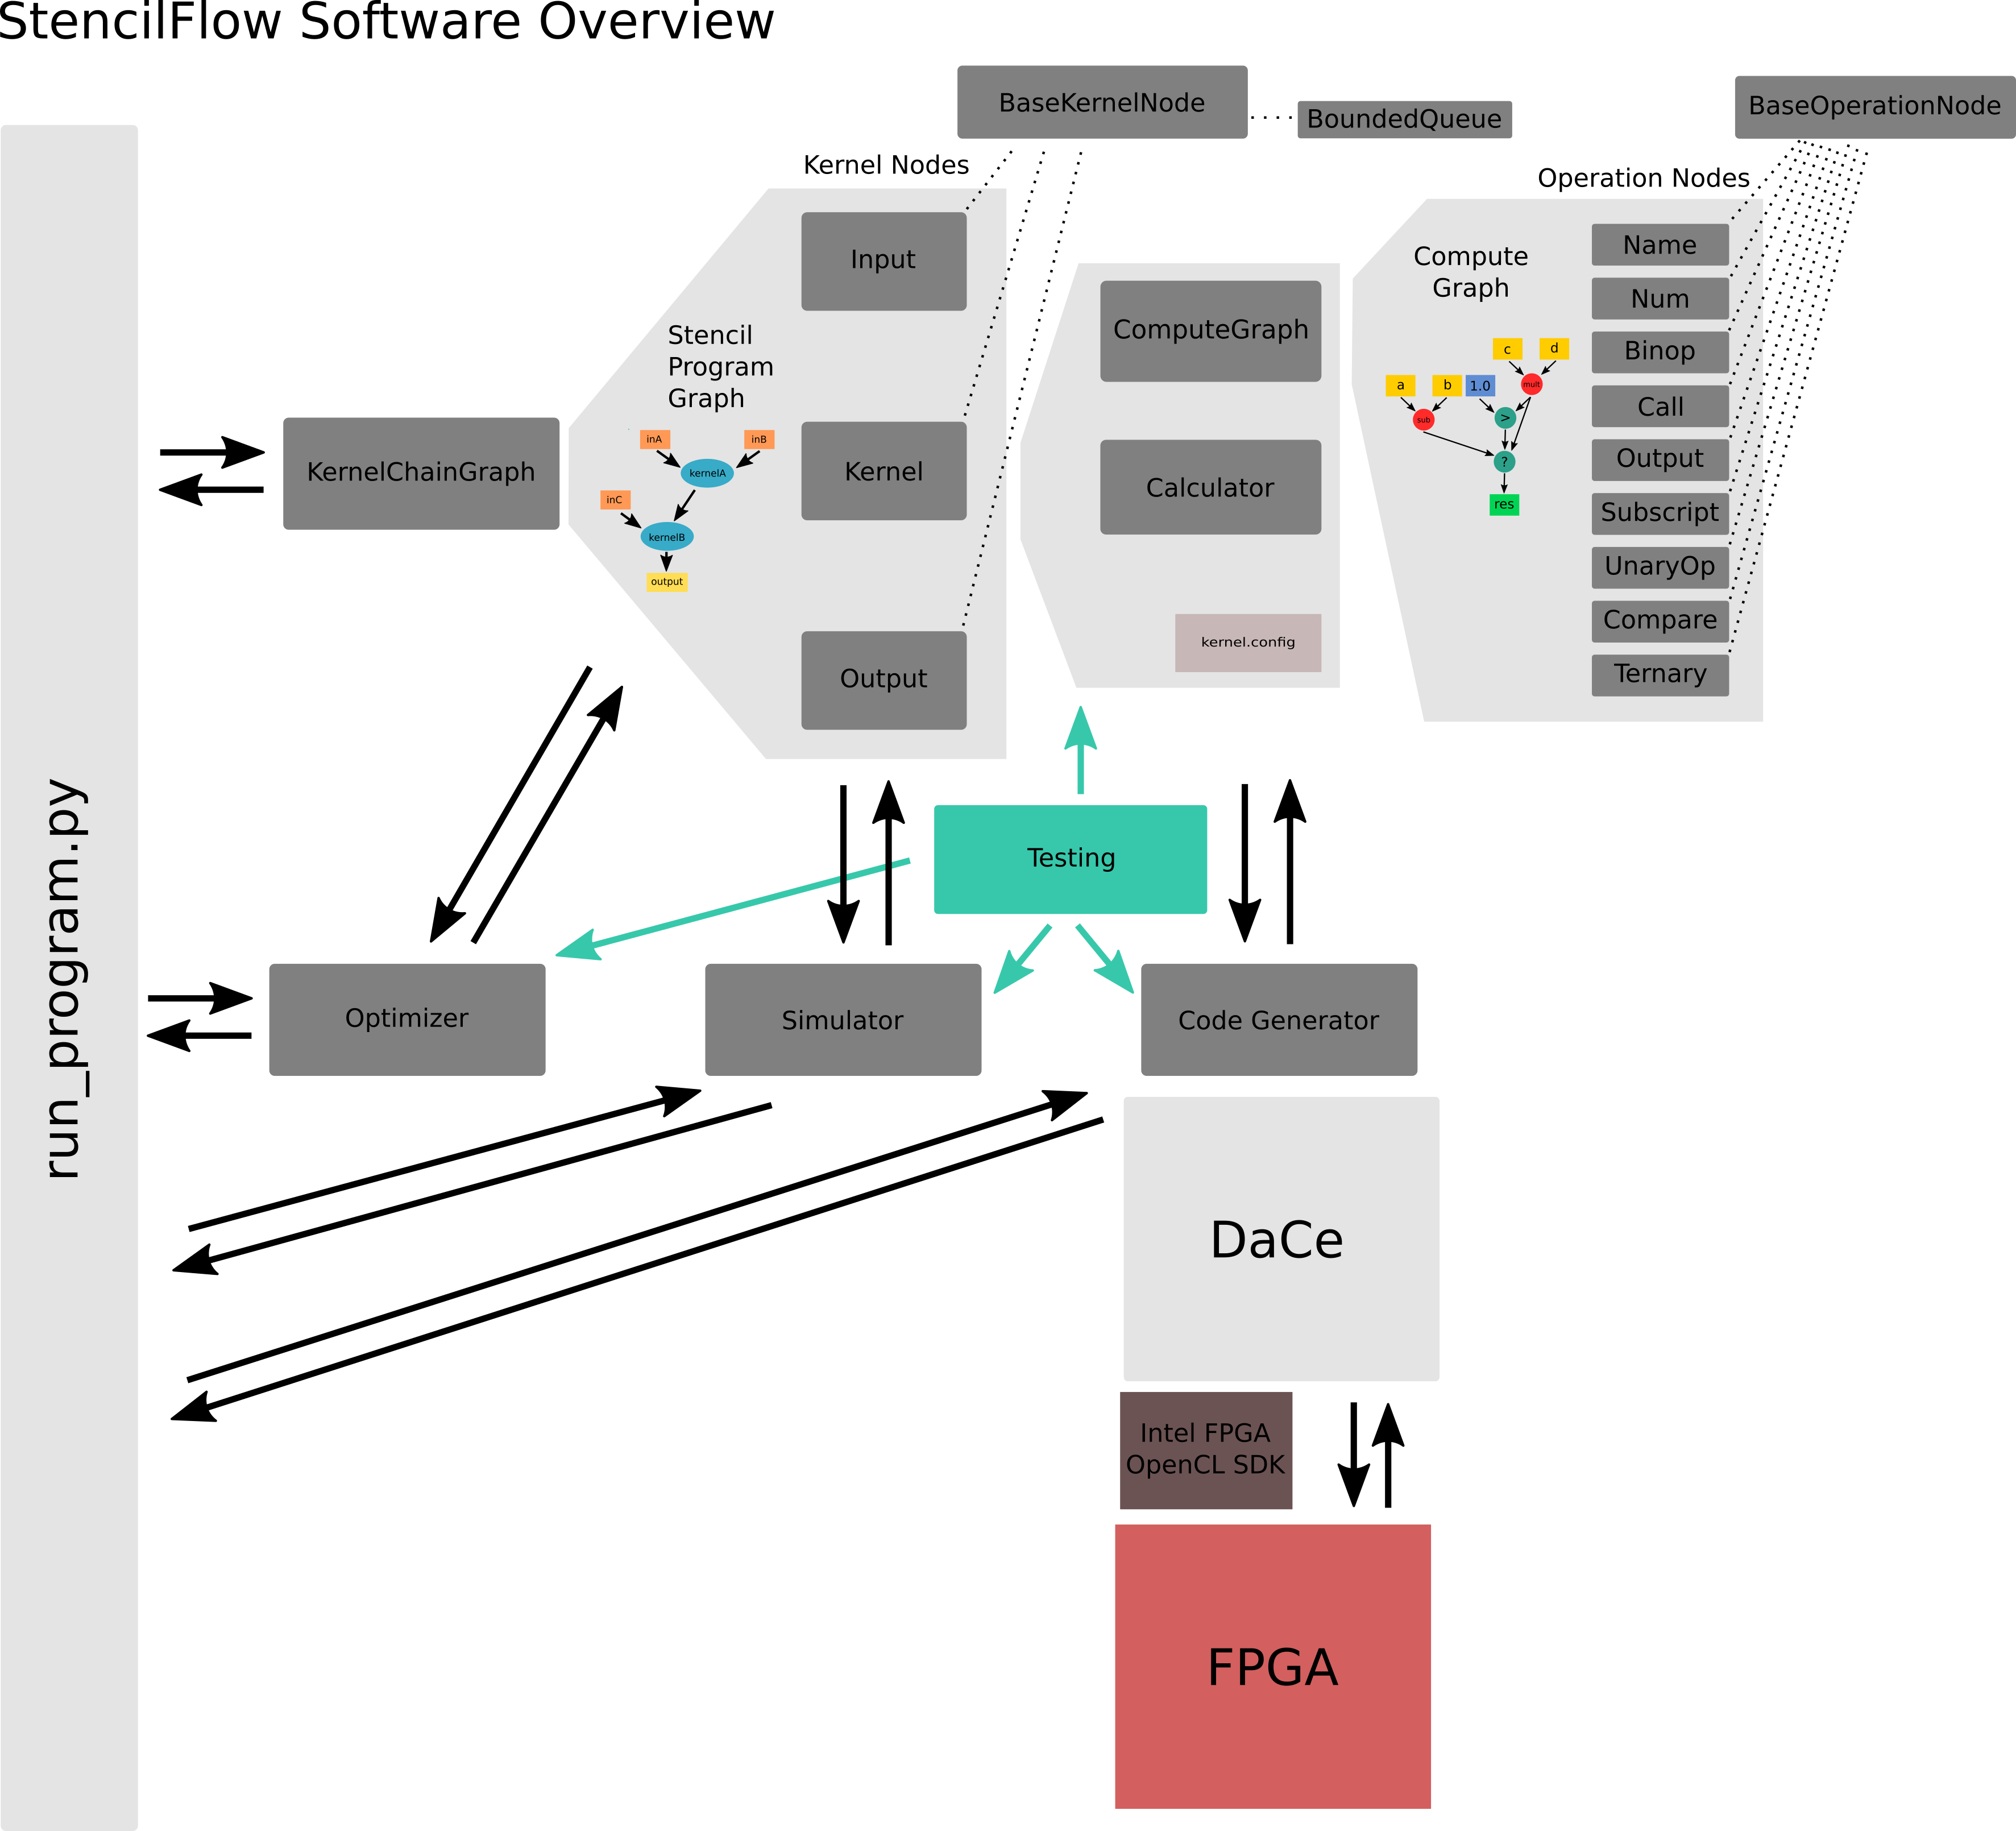
\includegraphics[height=24em]{drawings/implementation-class-overview.png}
	\caption{Overview of the StencilFlow class structure and their interaction.}
	\label{fig:implementation-class-overview}
\end{figure}
This section is dedicated to give you a detailed insight into the actual implementation with additional clarification why and how we implemented certain functionality.\\


This code snippet gives you an overview how the main classes interact with each other:
\begin{minted}{python}  
# instantiate the KernelChainGraph
chain = KernelChainGraph(path=args.stencil_file,
                         plot_graph=args.plot,
                         log_level=args.log_level)

# instantiate the Optimizer
opt = Optimizer(kernels=chain.kernel_nodes,
                dimensions=chain.dimensions,
                log_level=chain.log_level)
opt.optimize_to_ratio(1e-2)
    
# instantiate the Simulator
sim = Simulator(input_config_name=args.stencil_file
                chain=chain,
                write_output=False,
                log_level=args.log_level)
sim.simulate()
            
chain.report(args.stencil_file)
sim.report()
\end{minted}






\section{Input File}
The input json file contains all information required to analyze, optimize and run the given stencil program. We will go through its sections and explain them in detail.
\begin{minted}{json}
{
"inputs": {
    "inA": {
        "data": [
            19.30100000000000000e+00,
            19.43700000000000000e+00,
            19.30100000000000000e+00,
            19.03700000000000000e+00,
            19.36400000000000000e+00,
            19.31100000000000000e+00,
            19.93600000000000000e+00,
            20.10300000000000000e+00,
            20.24600000000000000e+00,
            20.03800000000000000e+00,
            20.36800000000000000e+00,
            20.03900000000000000e+00,
            20.24700000000000000e+00,
            20.03400000000000000e+00,
            20.10300000000000000e+00,
            20.56400000000000000e+00,
            20.94800000000000000e+00,
            19.19300000000000000e+00,
            19.36700000000000000e+00,
            19.98700000000000000e+00,
            20.43200000000000000e+00,
            20.95200000000000000e+00,
            21.34400000000000000e+00,
            21.07300000000000000e+00
        ],
        "data_type": "float64"
    },
    "inB": {
        "data": "inB.csv",
        "data_type": "float64"
    },
    "inC": {
        "data": "inC.dat",
        "data_type": "float32"
    }
},
"outputs": [
    "kernelB"
],
"dimensions": [
    2,
    3,
    4
],
"program": {
    "kernelA": {
        "computation_string": "out = 3.14 * (inB[i,j,k]-inB[i,j-1,k]);
                               res = (inA[i,j,k] + out) * cos(out);",
        "boundary_condition": {
            "inA": {
               "type": "constant",
               "value": 1.0
            },
            "inB": {
                "type": "constant",
                "value": 7.5
            }
        },
        "data_type": "float64"
    },
    "kernelB": {
        "computation_string": "res = kernelA[i,j,k] + inC[i,j,k];",
        "boundary_condition": {
            "kernelA": {
                "type": "copy"
            },
            "inC": {
                "type": "copy"
            }
        },
        "data_type": "float64"
    }
}
}
\end{minted}

\paragraph{Inputs}
The inputs section is dedicated to the input data arrays. For each input data array, there exists an entry that either contains data directly or references to an external file in binary or csv format. Furthermore, it specifies the data type and precision of the data.


\paragraph{Outputs}
The output section contains all kernel names of which data should not be discarted, but rather written back to the host computer as the output or computation result. This list can contain a single item or multiple entries.


\paragraph{Dimensions}
The dimensions value represents the global problem size and should correspond to the dimensions of the data arrays too (e.g. dimX*dimY*dimZ = size(input array)).


\paragraph{Program}
The program section contains information about the kernels of the stencil program. The computation\_string represents the kernel computation. The boundary condition subsection defines the condition per input in case of an out-of-bound data read. The data type specifies the precision of the computation. \\
\textit{Note: The precision value of data\_type might have severe performance impact  due to the impact in buffer requirements and the usage of hardened floating point operators.}






\section{Bounded Queue (bounded\_queue.py)}
The BoundedQueue class represents the basic building block when it comes to handle data in a FIFO manner. It can act as a feed to push data into the pipeline (input nodes), connect stencil chains as channels (internal and delay buffer), it does latency simulation within the kernel and collects all final results to store them on disk. We will go through the implementation details and explain for what the functionalities are useful. 

\begin{figure}[h]
	\centering
	
\includegraphics[height=8em]{drawings/implementation-bounded-queue.png}
	\caption{Working principle of the bounded queue implementation.}
	\label{fig:implementation-bounded-queue}
\end{figure}

\paragraph{Generic}
There are several short-cut implementations for generic functionality necessary to work with these data structures such as getting the actual size, check if the data structure is full respectively empty or print the basic instance info in a well-arranged way.


\paragraph{dequeue / try\_dequeue}
Removing and retrieving a single element from the BoundedQueue can be achieved using the dequeue method. The difference between the two implementations lies in the error handling. In case of an empty queue, dequeue raises an exception while the try\_dequeue method simply returns False instead of a data element in case of an empty queue. \\

There are valid use cases for both of them. For example in case of a kernel program trying to read data from input channels, that might or might not be available yet, try\_dequeue might be the better choice to avoid having to handle the exception.


\paragraph{enqueue / try\_enqueue}
Adding a single element to the BoundedQueue can be achieved using the enqueue method. The difference between the two implementations lies in the error handling. In case of a full queue, enqueue raises an exception while the try\_enqueue method simply discards the data item and indicates success or failure by the boolean return value. 


\paragraph{peek / try\_peek\_last}
The peeking functionality allows to retrieve items add arbitrary positions in the queue without actually removing them from the queue. Especially try\_peek\_last is very useful for the simulator to read the next element that is being feed into the kernel without actually touching the data.


\paragraph{import\_data / export\_data}
For the initial setup and cleanup we usually have to add many elements to a queue or retrieve all data elements from it. These functionalities are provided by the import\_data respectively export\_data methods.





\section{Calculator (calculator.py)}
The Calculator class provides the service of given a mathematical expression and a map from all variables to their corresponding values, to compute the numerical result of the expression, even for conditional expressions in the form of \textit{if(condition) true\_expression else false\_expression}. 

\paragraph{Internals}
The functionality is implemented by first parsing the expression into an abstract syntax tree. This tree is used later on to walk through and compute the intermediate values leading to the final result by having custom AST tree walker functions implemented. 
\begin{figure}[h]
	\centering
	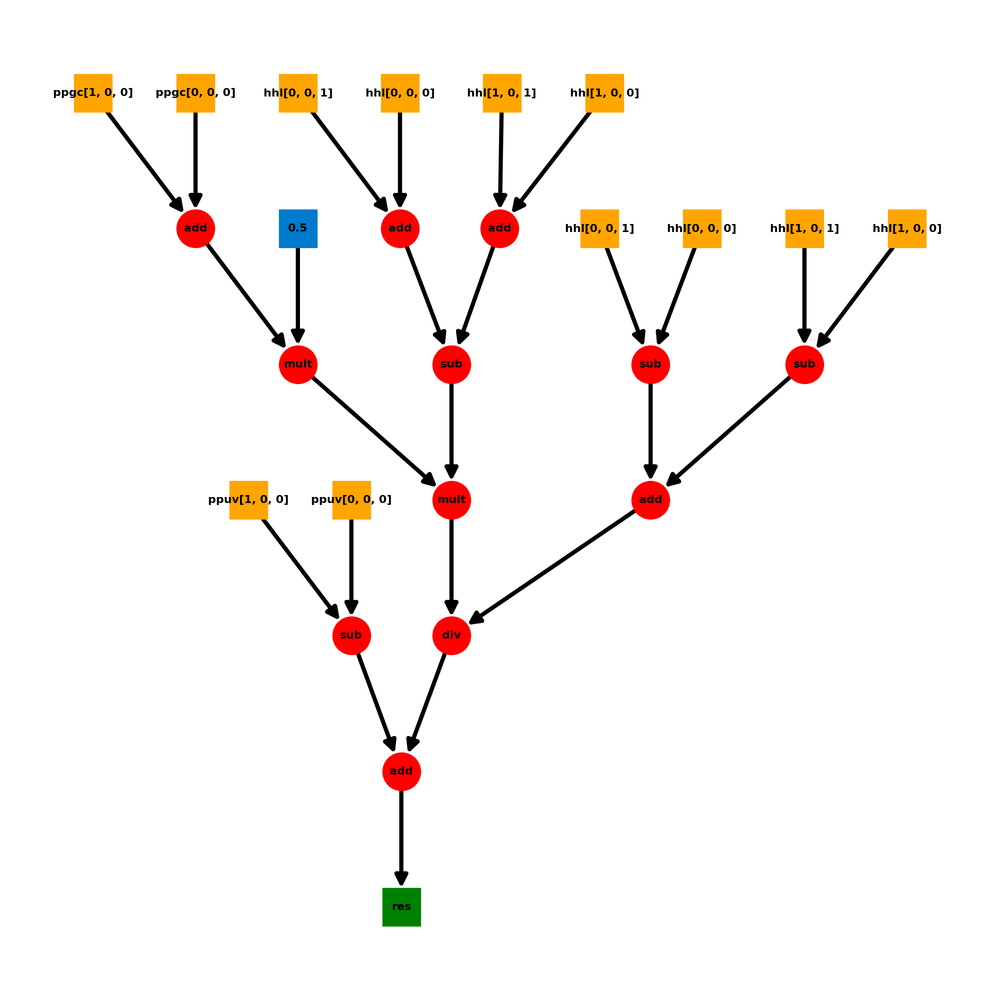
\includegraphics[height=16em]{images/compute-graph-example.png}
	\caption{Example of the high level visualization of a abstract syntax tree compute graph.}
	\label{fig:compute-graph-example}
\end{figure}


\paragraph{eval\_expr}
The Calculator class provides a single method for evaluation of an expressing. Given a mathematical expression and a map of all variable names to its corresponding value, the calculator computes the final result. This functionality is required for the simulator to be able to compute the kernel result, given all input values.


\paragraph{Example Usage}
The following example should illustrate the functionality of the Calculator class.
\begin{minted}{python}
variables = dict()                                
variables["a"] = 7                                
variables["b"] = 2                                

for var in variables:                             
  print("name: {}, value: {}"
        .format(var, str(variables[var])))

computation = "cos(-a + b) if (a > b) else (a + 5)
calculator = Calculator()                         
result = calculator.eval_expr(variables, computati
print("{} = {}".format(computation, str(result))) 
\end{minted}
Returns:
\begin{lstlisting}[showstringspaces=false, frame=single, language=Python]
name: a, value: 7
name: b, value: 2
cos(-a + b) if (a > b) else (a + 5) * b = 0.28366
\end{lstlisting}






\section{Compute Graph Nodes (compute\_graph\_nodes.py)}
The ComputeGraphNodes implement the BaseOperationNodeClass and are nodes of the ComputeGraph. Their main functionality beside have different nodes types in the three is to generate names and symbols for visualization from the given abstract syntax tree node. \\

\textit{Name}: The Name node class represents the variable name node in the computation tree. \\

\textit{Num}: The Num node class represents the numeral node (constant values) in the computation tree.\\


\textit{Binop}: The Binop node class represents the binary operations (e.g. addition, subtraction, etc.) in the computation tree.

\textit{Call}: The Call class represents the function calls (e.g. sin/cos,..) nodes in the computation tree. We support functions with single arguments, which could be extended to multiple argument functions if necessary.\\

\textit{Output}: The Output class represents the output node in the computation tree. \\

\textit{Subscript}: The Subscript class represents the array field access nodes in the computation tree. (e.g. inX[i,j,k+1]). It does convert the [i,j-2,k+1] index to relative number indices i.e. [0,-2,1] \\

\textit{Ternary}: The Ternary operator class represents ternary operation of the form:
expression\_true if comparison\_expression else expression\_false \\

\textit{Compare}: The Comparison operator class represents the comparison of two expression by a comparator (e.g $=, >=$, ..).

\textit{UnaryOp}: The UnaryOp operator class represents unary operations. In our case we only support negation (mathematical - sign) as unary operation yet.





\section{Compute Graph (compute\_graph.py)}
The ComputeGraph class represents the actual computation of a kernel instance. It analyses the field access patterns and metrics such as the critical path latency. Furthermore, it generates a high-level graph representation from the input fields through the computational nodes to the output, which can be visualized nicely.


\paragraph{Configuration}
Performance metrics such as latency greatly depends on the underlying FPGA hardware. This is why we did not hard-code such values, but rather provide the flexibility to load the configuration of operation latency values at runtime. 
\begin{minted}{json}
{
"op_latency": {
	"add": 16,
	"sub": 16,
	"mult": 16,
	"div": 128,
	"inv": 16,
	"sin": 128,
	"cos": 128,
	"tan": 128,
	"sinh": 128,
	"coshh": 128,
	"comparison": 16,
	"conditional": 16,
	"neg": 16
	}
}
\end{minted}


\paragraph{Nodes}
The computation graph contains several different node types, each of them represents either a data source, a data destination or some type of computation.
\begin{itemize}
	\item Name: variable names
	\item Num: numeral (constant number)
	\item Binop: binary operation (e.g. addition, subtraction etc.)
	\item Call: function call (e.g. sin(), cos(), etc.)
	\item Output: output/result node
	\item Subscript: array access (e.g. inX[i,j,k+1])
	\item Ternary: ternary (conditional) operation node of the form: if\_expr if condition else else\_expr
	\item Compare: part of the ternary operator, tests the condition
	\item UnaryOp: unary operations (e.g. negation)
\end{itemize}


\paragraph{setup\_internal\_buffers}
This method takes care of computing the internal buffer size. This can be achieved by first finding the highest and the lowest access index per field and compute the difference which is exactly the internal buffer size plus one. internal buffer size(field) = max\_field\_access(field) - min\_field\_access(field) + 1.


\paragraph{Data Reuse, Multiple Expressions}
There are many cases where part of the kernel expression is occurring more than one time. For efficiency reasons, it makes sense to compute them only once. We provide this functionality by allowing to split the expression into subexpression, which can be referenced multiple times. This can be achieved using the following syntax: "res = -a if (a+1 $>$ b-c) else b; b = d + e" where b is being substituted twice by (d + e). \\
From the implementation perspective, we have to account for the processing of both parts of the expression as well as contracting the output node b (from b = d + e) with the input node b (in res = -a if (a+1 $>$ b-c) else b;), which is being achieved by the contract\_edge method.


\paragraph{generate\_graph}
The generate\_graph method creates a high-level networkx graph consisting of OperationNodes for further visualization and analysis. The expression is parsed using the abstract syntax tree framework which gives us the ability to walk through the AST tree in order to extract all the required information.
The ast\_tree\_walk method is a recursive method that does the following steps:
\begin{enumerate}
	\item create a new node from node and the node number and add it to the graph
	\item depending on the type of node, call ast\_tree\_walk recursively for left child (node number: 2*parent + 1) and right child (node number: 2*parent)
	\item add edge from the new node to the recursive 
	child/children
	\item return new node
\end{enumerate}
% ref to networkx


\paragraph{plot\_graph}
Visualizing the problem instances greatly helps to get a good understanding of the problem and seeing what is going or what we could further optimize. This method accounts for that by plotting a well-arranged overview of the ComputeGraph. 
\begin{figure}[h]
	\centering
	\includegraphics[height=16em]{images/compute-graph-debugging-example.png}
	\caption{Example of the high level visualization of a abstract syntax tree compute graph.}
	\label{fig:compute-graph-debugging-example}
\end{figure}


\paragraph{calculate\_latency}
The latency of the critical path is a key metric for our problem question and part of the ComputeGraphs functionality. This can be achieved by a recursive tree walk from the output node up to the field accesses while carrying out the latency propagation i.e. latency\_to\_outp(child) = max\{latency\_to\_outp(child), latency\_to\_outp(self) + operation\_latency(self)\}
\textit{Remark: The reason for using the maximum of both values is that the tree is not a classical mathematical tree, but rather a directed acyclic graph. It can happen due to the allowance of substitution/reuse of identical part of the computation to have a cycle if we look at it as an undirected graph. This behavior can be seen by the example ComputeGraph above.}







\section{Base Node (base\_node\_class.py)}
The base node class is not a class by itself, but rather contains the abstract base nodes for the ComputeGraph and the KernelChainGraph. \\


\paragraph{BaseKernelNodeClass}
The BaseKernelClass provides all the basic fields and functionality for its subclasses which are the Input, Kernel and Output classes. These are nodes of of the KernelChainGraph. \\
Furthermore, it provides a fall-back implementation of the generate\_label functionality.


\paragraph{BaseOperationNodeClass}
The BaseOperationNodeClass class provides all the basic fields and methods for its subclasses (Num, Subscript,..). These are the nodes of the ComputeGraph.\\
Furthermore, it provides a fall-back implementation of the generate\_label and functionality. In addition, it contains an method generate\_name to generate the node name from the AST node, which all subclasses have to implement.








\section{Input (input.py)}
The Input class is a subclass of the BaseKernelNodeClass and represents an Input node in the KernelChainGraph. Its purpose is to feed input data into the pipeline/data flow design. 


\paragraph{init\_queues}
This method sets up a dedicated queue for each output channel. This is necessary since some of the kernels might have to wait for other inputs to get available till they start reading from this channel.


\paragraph{try\_write}
This method is called by the simulator in the step execution cycle. The input node loops over all output channels and tries to add a data element to them. If the corresponding data queue is already empty (all elements already feed) it inserts a "bubble" (None) in order to keep the data flow running. If the output channel is full, it does nothing. 
\begin{figure}[h]
	\centering
	\includegraphics[height=16em]{drawings/inputs-multi-queue.png}
	\caption{The functionality of the Input node. Feed each channel individually.}
	\label{fig:inputs-multi-queue}
\end{figure}


\paragraph{init\_input\_data}
The init\_input\_data method initializes the internal queues with data from the config file or the file system. It currently supports the following file types: implicit (array defined in the input config file), binary (.dat, .bin, .data) , h5 and csv.







\section{Output (output.py)}
The Output class is a subclass of the BaseKernelNodeClass and represents an Output node in the KernelChainGraph. Its purpose is to store data coming from the pipeline/dataflow design. 


\paragraph{try\_read}
This method is called by the simulator in the step execution cycle. It simply tries to read from the input channel and stores the element into the data\_queue on success.


\paragraph{write\_result\_to\_file}
The write\_result\_to\_file method writes the content of the internal queue with the computation results to the binary file at \textit{results/INPUT\_CONFIG\_NAME/SELF.NAME\_simulation.dat}. This can be used for example to compare the simulator values with the result coming from the actual hardware implementation.







\section{Kernel (kernel.py)}

\paragraph{Overview}
The Kernel class is used for four different scenarios:
\begin{enumerate}
	\item Initialization: setup and computation of buffer sizes and latencies.
	\item Optimization: set/reset swap out buffer flags
	\item Simulation: run data through the data flow graph by repeatedly calling try\_read/try\_execute and try\_write
	\item Code Generation: extraction of equations and buffer swap out flag
\end{enumerate}


\subparagraph{Initialization}
The initialization phase looks like:
\begin{enumerate}
	\item instantiate Calculator class
	\item instantiate ComputeGraph class with given compute\_string
	\item generate compute graph (networkx data structure)
	\item compute compute graph latency (critical path)
	\item compute and set up internal buffers
	\item set up latency simulation out delay queue
	\item compute access distance from furthest access to the center
\end{enumerate}


\subparagraph{Optimization}
The optimization framework takes kernels as input and sets or resets the field \textit{swap\_out} of the delay buffer or internal buffer parts to indicate whether or not the buffer should stay in fast memory.


\subparagraph{Simulation}
The simulator makes us of the pre-defined step execution calls \textit{try\_read, try\_execute} and \textit{try\_write}. 


\subparagraph{Code Generation}
The code generator makes use of the function \\*
\text{generate\_relative\_access\_kernel\_string} that transforms the input compute\_string with given global dimensions to a single dimensional index based string.
\begin{lstlisting}[showstringspaces=false, frame=single, language=Python]
dimensions are: [100, 100, 100]
input: res = a[i+1,j+1,k+1] + a[i+1,j,k] + 
             a[i-1,j-1,k-1] + a[i+1,j+1,k] + 
             (-a[i,j,k])
relative_access_kernel_string: res = ((((a[0] +
             a[-101]) + a[-20202]) + a[-1]) + 
             (-a[-10101]))
\end{lstlisting}



\paragraph{print\_kernel\_performance}
This methods pretty-prints the performance metrics (maximum buffer usage, average buffer usage, total execution time, etc) gathered during the simulation. 


\paragraph{update\_performance\_metric}
This method is called by the simulator every step execution in order to gather and process internal state metrics.


\paragraph{set\_up\_dist\_to\_center}
Computes for all fields/channels the distance from the furthest field access to the center of the stencil ([0,0,0]). \\ 
This is necessary and covers the following edge case: Suppose we have the kernel: \textit{out[i,j,k] = in[i,j,k-2] + in[i,j,k+2]} without accessing the center element (in[i,j,k]) from the input. We look at the time two step execution cycles before the first actual execution of this kernel with valid input data. The front access is already in the position to read valid data while the back access is in the boundary condition which can lead to an invalid execution (if no center access is used it seems to be valid but in fact is not). In order to circumvent this, we introduce the distance-to-center and decrement it every step to make sure we start as soon as the center element is in the first position.  
\begin{figure}[h]
	\centering
	\includegraphics[height=8em]{drawings/software-dist-to-center.png}
	\caption{Edge Case: Distance to center.}
	\label{fig:software-dist-to-center}
\end{figure}


\paragraph{iter\_comp\_tree}
This method iterates through the computation tree in order to generate the kernel string (according to some properties e.g. relative to center or replace negative index. The pseudo code for the function is:
\begin{algorithm}
	\caption{iter\_comp\_tree(node)}
	\begin{algorithmic}
		\STATE get all predecessors pred
		\STATE check what type of Node node is
		\STATE depending on the node type, recursively call iter\_comp\_tree for the predecessor(s)
		\STATE return the formated string e.g. for binary operation: LHS op RHS
	\end{algorithmic}
\end{algorithm}
\textit{Relative to center: The absolute array index value is either relative to the center node e.g. center is at 0 and [i,j,k+10] is at [10] or relative to the front access e.g. the center is at [-10] and [i,j,k+10] is at [0].}
\\
Replace negative index: In order to get a valid variable name string, we have to replace the negative sign '-' by 'n' otherwise it gets interpreted as a mathematical symbol (for the Calculator class) e.g. arrA\_-20 gets replaced by arrA\_n20


\paragraph{generate\_relative\_access\_kernel\_string}
Generates the relative (either to the center or to the furthest field access) access kernel string which is necessary for the code generator HLS tool.


\paragraph{reset\_old\_compute\_state}
This is a helper function for the simulator to make sure that no artifacts from any previous simulation step is remaining. It clears the variable to value map and all execution related flags such as read\_success.


\paragraph{convert\_3d\_to\_1d}
Converts [i,j,k] to a flat 1D array index using the given dimensions [dimZ, dimY, dimX] using the formula:
index = i*dimY*dimX + j*dimX + k = (i*dimY + j)*dimX + k (dimensional to absolute value formula from the model part).


\paragraph{remove\_duplicate\_accesses}
The list of field accesses must be cleaned from duplicate entries, since they can be handled concurrently and could increase the complexity of the computations of StencilFlow.


\paragraph{setup\_internal\_buffers}
This method creates and splits the internal buffers according to the pipeline model. Each internal buffer part has the length from one access of the field to the next. This is done in the following way:
\begin{algorithm}
	\caption{setup\_internal\_buffers}
	\begin{algorithmic}
		\STATE sort all buffer accesses in the list
		\STATE case single buffer access: internal buffer is size 1
		\STATE case multiple buffer accesses: iterate over the list
		\STATE compute difference from current to next access
		\STATE create buffer of this size and add it to the buffers
	\end{algorithmic}
\end{algorithm}


\paragraph{buffer\_number}
Computes the index position of the internal buffer part from the access position. \\
\textit{Example: out[i,j,k] = in[i,j,k-10] + in[i,j,k] + in[i,j,k+10] has two internal buffers (form k-10 to k, and from k to k+10). The data item for the access [i,j,k+10] comes from the delay buffer, the one for [i,j,k] form the first internal buffer and for [i,j,k-10] from the second internal buffer. If we call buffer\_position([i,j,k+10]) we get '-1' which indicates the delay buffer. For buffer\_position([i,j,k]) we get '0' and for buffer\_position([i,j,k-10]) we get '1'}


\paragraph{get\_global\_kernel\_index}
Return the current position (simulator, program counter) within the computation as a list of the form [i,j,k]. This is required for the simulation to test if the data at a specific index is out-of-bound or not.\\
\textit{Example: global problem size: [2,3,4]. \\
	(1) Current program counter index: 3, global kernel index: [0,0,3] \\
	(2) Current program counter index: 7, global kernel index: [0,1,3]}


\paragraph{is\_out\_of\_bound}
Checks whether the current access is within bounds or not. This is required for the simulation to check if boundary conditions must be applied or regular data should be read.


\paragraph{get\_data}
Returns data of current stencil access (could be real data or boundary condition)


\paragraph{test\_availability}
This method checks if all accesses are available (and ready for execution). In addition, the method returns all accesses that are not available yet. Checks are different for different data types:

\subparagraph{Numeral (Constant Values)}
They are always available and therefore nothing has to be checked.

\subparagraph{Subscript (array) data accesses}
The buffers have to be checked if data is ready yet:
\begin{algorithm}
	\caption{setup\_internal\_buffers}
	\begin{algorithmic}
		\STATE peek the last element of the delay buffer
		\STATE peek the last element of all internal buffer junks
		\IF {none of the is 'None'}
		\STATE all data elements are available
		\ELSE
		\STATE not all items are available yet
		\ENDIF
	\end{algorithmic}
\end{algorithm}


\paragraph{move\_forward}
Moves all items within the internal and delay buffer one element forward to free up space for a new data element. The furthest element is getting discarded since it is not used anymore.  
\begin{figure}[h]
	\centering
	\includegraphics[height=12em]{drawings/implementation-move-forward.png}
	\caption{Move data forward.}
	\label{fig:implementation-move-forward}
\end{figure}


\paragraph{decrement\_center\_reached}
This counter (individual to each field) gets decremented every time there is a data item at the output of the delay buffer (kernel access index position [0,0,0]). The counter reaching zero indicates that the kernel reached center for this field.


\paragraph{try\_read}
This is the implementation of the kernel reading functionality of the simulator. It tries to read from all input channels and indicates if this has been done with success. It does the following procedure written in pseudo code:
\begin{algorithm}
	\caption{try\_read}
	\begin{algorithmic}
		\STATE check if all inputs are available
		\STATE case success: read all data items into the variable to value map var\_map and set the read\_success flag
		\STATE case unsucessful: reset the read\_success flag
		\STATE decrement the center counter for all fields that have data at the output of the delay queue
		\STATE check if all counter reached 0
		\STATE case true: continue
		\STATE case false: move all delay/internal buffer forward for the fields that did not reach center yet
	\end{algorithmic}
\end{algorithm}

\paragraph{try\_execute}
This is the implementation of the kernel execution functionality of the simulator. It executes the stencil computation for the current variable mapping that was set up by the try\_read() function. It does the following procedure written in pseudo code:
\begin{algorithm}
	\caption{try\_execute}
	\begin{algorithmic}
		\IF {check if center has been reached, read\_success is set and the internal program counter is between 0 and PROBLEM\_SIZE}
		\STATE get the relative access kernel string
		\STATE compute the result of the expression together with the variable map using the calculator
		\STATE add result to out\_delay\_queue
		\STATE increment the program counter
		\ELSE
		\STATE add a None (bubble) to the out\_delay\_queue
		\ENDIF
	\end{algorithmic}
\end{algorithm}


\paragraph{try\_write}
This is the implementation of the kernel write functionality of the simulator.  It does the following procedure written in pseudo code:
\begin{algorithm}
	\caption{try\_write}
	\begin{algorithmic}
		\STATE dequeue last element from the out\_delay\_queue
		\STATE add it to the input channel of all kernel outputs respectively successor nodes
	\end{algorithmic}
\end{algorithm}

\paragraph{diagnostics}
The diagnostics method summarizes the internal kernel state. It either gets called upon an exception or at the end for the final report. It provides the following information:
\begin{itemize}
	\item program counter
	\item all\_available flag
	\item center\_reached
	\item exception traceback
	\item Inputs/Outputs:
	\begin{itemize}
		\item delay buffer maximal size
		\item delay buffer current size
		\item delay buffer content
		\item internal buffer content
	\end{itemize}
	\item content of latency simulation buffer (out\_delay\_queue)
\end{itemize}


\paragraph{out\_delay\_queue}
The out\_delay\_queue's purpose is to simulate the computation latency of the computation graph. This is achieved by having a FIFO queue of length \textit{max\_latency} and by adding each result to the queue while sending out the last item from the queue each cycle instead of directly sending it out.







\section{Kernel Chain Graph (kernel\_chain\_graph.py)}
The KernelChainGraph class represents the whole pipelined data flow graph consisting of input nodes (real data input arrays, kernel nodes and output nodes (storing the result of the computation).


\paragraph{Call}
The KernelChainGraph can be called in the following way:
\begin{minted}{python}
python3 kernel_chain_graph.py -stencil_file stencils/simulator12.json -plot -simulate 
    -report -log-level 2
\end{minted}

\paragraph{Initialization}
The following procedure is called to initially setup the internal structure and analyze the input configuration:
\begin{enumerate}
	\item set up all internal data structures (dicts, lists,..)
	\item read input config files
	\item create all kernels
	\item compute kernel latencies
	\item connect kernels in the graph
	\item compute delay buffer sizes
	\item add channels to the graph edges
	\item plot all graphs (if flag set)
\end{enumerate}

\paragraph{plot\_graph}
Visualizing the stencil program instances greatly helps to get a good understanding of the problem and seeing what is going or what we could further optimize. This method accounts for that by plotting a well-arranged overview of the StencilChainGraph. 
\begin{figure}[h]
	\centering
	\includegraphics[height=24em]{images/fastwaves.png}
	\caption{Example stencil chain graph.}
	\label{fig:fastwaves}
\end{figure}


\paragraph{connect\_kernels}
This method connects all networkx nodes to a directed acyclic graph by matching the input names with the corresponding kernel names.


\paragraph{add\_channels}
Add\_channels packs all required information (name, delay buffer queue, internal buffer queue and data type) into a dictionary and adds it to the edge between the corresponding two nodes of the graph.
\begin{minted}{python}     
channel = {
  "name": name,
  "delay_buffer": self.kernel_nodes[dest.name].
                  delay_buffer[src.name],
  "internal_buffer": dest.internal_buffer[src.name],
  "data_type": src.data_type
}
\end{minted}


\paragraph{import\_input}
This helper method reads the input file and adds each part to the corresponding field in the class.


\paragraph{total\_elements}
Reduces the global problem size to a single scalar value.


\paragraph{create\_kernels}
Instantiates the kernels and adds them to the networkx graph.


\paragraph{compute\_kernel\_latency}
Fills a global dictionary of the individual critical kernel computation paths.


\paragraph{compute\_delay\_buffer}
Computes the delay buffer sizes in the graph by propagating all paths from the input arrays to the successors in topological order. Delay buffer entries should be of the format: kernel.input\_paths:{
	"in1": [[a,b,c, pred1], [d,e,f, pred2], ...],
	"in2": [ ... ],
	...
}
where inX are input arrays to the stencil chain and predY are the kernel predecessors/inputs. This is being achieved in the following way:
\begin{algorithm}
	\caption{compute\_delay\_buffer}
	\begin{algorithmic}
		\STATE sort the graph in topological order
		\STATE go over all nodes in the topological order
		\STATE process delay buffers (no new delay buffers can occur since its is topologically sorted)
		\STATE max delay = maximum entry for this field
		\STATE compute delay buffer for all field by subtracting it from the maximum one (the maximum one does not require a delay buffer since it is ready as the last one)
		\STATE propagate the path length as own path length + internal delay from computation and delay buffers
	\end{algorithmic}
\end{algorithm}

\begin{figure}[h]
	\centering
	\includegraphics[height=16em]{drawings/software-delay-buffer.png}
	\caption{Example delay buffer computation using the path accesses list.}
	\label{fig:software-delay-buffer}
\end{figure}


\paragraph{compute\_critical\_path\_dim}
Computes the maximum latency critical path through the graph in dimensional format. \\
\textit{Note: Since we know the output nodes as well as the path lengths the critical path is simply
	max \{ latency(node) + max \{ path\_length(node) | node in output nodes \}\} }


\paragraph{report}
The report summarizes the stencil program information and analysis and reports the following information:
\begin{itemize}
	\item dimensions of data array (problem size)
	\item channels
	\item data field accesses
	\item internal buffer size
	\item internal buffer chunks
	\item delay buffer size
	\item path lengths (from the input to the node, per field)
	\item latency
	\item total buffer 
	\item input kernel string
	\item relative access kernel string
	\item slow and fast memory buffer size
\end{itemize}







\section{Simulator (simulator.py)}
The Simulator class handles the simulation of our high level model FPGA functionality of the stencil chain design as described in the model section (figure \ref{fig:simulator-simulation-cycle}). \\


\paragraph{simulate}
The simulate orchestrates the simulator and does the following:
\begin{algorithm}
	\caption{simulate}
	\begin{algorithmic}
		\STATE initialize: read all data into input nodes
		\STATE set global program counter PC=0
		\WHILE {not all input/kernel/output nodes done}
		\STATE step execution()
		\STATE PC = PC + 1
		\ENDWHILE
		\STATE finalize: write all output data to file
	\end{algorithmic}
\end{algorithm}

\paragraph{step\_execution}
A single step of the step\_execution represents a single cycle on an FPGA, split up into sub-steps, which are being called into the Input, Kernel and Output classes as follows:
\begin{algorithm}
	\caption{step\_execution}
	\begin{algorithmic}
		\STATE try\_read all output and kernel nodes
		\STATE try\_execute all kernel nodes
		\STATE try\_write all input and kernel nodes
	\end{algorithmic}
\end{algorithm}

\paragraph{initialize}
The initialization method does the pre-processing before the actual simulation. It takes cares care of importing the input data.


\paragraph{finalize}
The finalization method does the post-processing after successful simulation. It writes the result data to a file and outputs the performance metrics if the log-level is at least 'basic'.


\paragraph{get\_result}
The get\_result functionality allows to extract the simulation result of the stencil program to be extracted.


\paragraph{all\_done}
This method checks if all nodes have finished their execution and are idling. This is achieved by adding a local, node-internal program counter that increments whenever there has been a successful execution of an operation. For the input nodes it means: problem\_size - largest queue = program counter or in other words, as soon as the last queue is empty, the program counter reached the value of dimX*dimY*dimZ. For the kernel nodes a increment of the program counter happens after a successful execution. A program counter increment for the output node happens after a successful data read. \\
As soon as all the program counter reached the value of the problem size, we can safely terminate. Since this is a sufficient and required property, this is an efficient implementation without doing any unnecessary idle steps.


\paragraph{diagnostics}
Diagnostics in the simulator is not only an exception handler, but is actually of great importance for the whole StencilFlow tool since most of the exceptions happen because of wrong input assumptions or wrong buffer size calculations.\\
Therefore, the diagnostics exception handler does not only raise the exception, but rather starts a procedure where the current state of all nodes (input, kernel and output) is being post-processed and logged. The diagnostics function of these nodes is being called and an output log including current program counter, internal state properties (e.g. for kernel: all\_available, center\_reached, etc) and channel/buffer content is displayed. Which helps for later analysis and finding the root cause of the error.


\paragraph{report}
If the log-level is at least 'basic', a report about the internal node state is generated after the simulation successfully completed, exactly as in the diagnostic method but just without an actual exception.






\section{Optimizer (optimizer.py)}
The Optimizer class is a key piece of StencilFlow and takes care of the optimal allocation and usage of the optimization parameters: fast memory, slow memory and bandwidth. 



\paragraph{single\_comm\_volume}
This method returns the number of bytes necessary to copy a whole data array from or to the FPGA. This number actually corresponds to: dimX*dimY*dimZ * 4 bytes.


\paragraph{add\_buffers\_to\_metric}
Creates the buffer data structure for optimization. It not only stores the information about the individual buffer, its communication volume and data type, but also maintains a doubly linked list to its predecessor and successor for updating the communication volume in case of a swap\_out of a buffer.
\begin{minted}{python}
{
    "queue": entry,
    "comm_vol": 2*self.single_comm_volume(
        self.kernels[kernel].data_type.bytes),
    "type": "internal",
    "datatype_size": self.kernels[kernel].data_type.bytes,
    "prev": prev,
    "next": None
}
\end{minted}


\paragraph{max\_metric}
This method finds the buffer entry in the metric\_data list with the maximum metric value i.e. the buffer with the highest ratio: $\frac{buffer size}{communication volume}$ that is still located in fast memory.


\paragraph{ratio}
Computes the ratio between fast memory and the communication volume of the current optimization state. This is useful for the \textit{optimize\_to\_ratio} optimization strategy.


\paragraph{update\_comm\_vol}
This method is being called for both neighbors if we moved a fast memory buffer to the slow memory. It updates the communication volume according to the formula derived in the model section according to the following rule:
\begin{lstlisting}[showstringspaces=false, frame=single, language=Python]
How to determine the necessary communication volume?
(predecessor, successor):
case (fast, fast): 2*C
case (fast, slow): C
case (slow, fast): C
case (slow, slow): 0
where C:= communication volume to stream single data
    array in or out of fast memory (=SIZE(data array))
\end{lstlisting}
\textit{Note: pred of delay buffer is always fast memory since the stream from the predecessor kernel is being compute on the FPGA die next to the fast memory.}


\paragraph{minimize\_comm\_vol}
This optimization strategy optimizes the problem to minimize the communication volume between fast and slow memory. In other words, it uses as little bandwidth as possible by a given amount of fast and slow memory. This implies that this strategy makes maximal use of the fast memory. The pseudo code for this function is:
\begin{algorithm}
	\caption{minimize\_comm\_vol(fast\_memory\_bound, slow\_memory\_bound)}
	\begin{algorithmic}
		\STATE mark all buffers to be allocated in fast memory
		\WHILE {metric\_data list is not empty and fast\_memory\_use > fast\_memory\_bound}
		\STATE swap max metric buffer to slow memory
		\STATE update neighbors
		\STATE remove buffer from metric\_data
		\STATE update fast memory, slow memory and bandwidth use
		\IF {check if slow\_memory\_use > slow\_memory\_bound}
		\STATE Exception
		\ENDIF
		\ENDWHILE
	\end{algorithmic}
\end{algorithm}

\textit{Note: The above exception occurs if the total buffer memory consumption is higher than sum of the slow memory and fast memory bound, which means that there cannot be found any solution for this optimization problem.}


\paragraph{minimize\_fast\_mem}
This optimization strategy minimizes the usage of fast memory by a given amount of communication volume from/to slow memory. This implies that strategy makes maximal use of the available memory bandwidth and slow memory. The pseudo code for this function is:
\begin{algorithm}
	\caption{minimize\_fast\_mem(communication\_volume\_bound, slow\_memory\_bound)}
	\begin{algorithmic}
		\STATE mark all buffers to be allocated in fast memory
		\WHILE {metric\_data list is not empty and comm\_volume\_use > comm\_volume\_bound and slow\_memory\_use < slow\_memory\_bound}
		\STATE swap max metric buffer to slow memory
		\STATE update neighbors
		\STATE remove buffer from metric\_data
		\STATE update fast memory, slow memory and bandwidth use
		\ENDWHILE
	\end{algorithmic}
\end{algorithm}

\paragraph{optimize\_to\_ratio}
This optimization strategy optimizes for the given ratio value between the fast memory usage and the amount of available communication volume. The pseudo code for this function is given by:
\begin{algorithm}
	\caption{optimize\_ratio(ratio)}
	\begin{algorithmic}
		\STATE mark all buffers to be allocated in fast memory
		\WHILE {metric\_data list is not empty and current\_ratio > ratio}
		\STATE swap max metric buffer to slow memory
		\STATE update neighbors
		\STATE remove buffer from metric\_data
		\STATE recompute current\_ratio
		\STATE update fast memory, slow memory and bandwidth use
		\ENDWHILE
	\end{algorithmic}
\end{algorithm}

\paragraph{report}
The optimizer report gives an overview of the important metric values such as:
\begin{itemize}
	\item swap status: which buffers are swapped out to slow memory and which are allocated in fast memory
	\item fast memory usage (for the strategy we optimized for)
	\item slow memory usage (for the strategy we optimized for)
	\item communication volume usage (for the strategy we optimized for)
\end{itemize}







\section{SDFG Generator (sdfg\_generator.py)}
The Stateful DataFlow multiGraph (SDFG) Generator is the interface between the high-level representation in StencilFlow and the low-level and hardware design generator in DaCe \cite{label57}. This part has been implemented by my mentor Johannes de Fine Licht.







\section{Run Program (run\_program.py)}
Run\_program is a wrapper program that instantiates all required components and classes in order to run the input stencil program with the given input data arrays in software or hardware as specified by the arguments. Furthermore, we can simulate the design using StencilFlow and check if the output matches.
\begin{enumerate}
	\item read program input file
	\item create the kernel chain graph (including analysis of buffer sizes, latencies, etc)
	\item execute the optimizer
	\item execute the simuator and store the result
	\item generate HLS OpenCl code from the high-level representation (using SDFG)
	\item compile the code
	\item read input data arrays
	\item run the design in hardware (or in the Intel SDK Simulation Mode)
	\item compare the result to the output from the simulator and check if they match
\end{enumerate}

\textit{Note: In order to run the design on the actual hardware, we have to do the synthesis from the OpenCL code to the actual hardware bitstream. This is being done separately since we have to do this only once and since it takes many hours and should therefore not block the very limited number of nodes with hardware FPGAs installed.}


\section{Helper (helper.py)}
The helper name space does not contain any specific classes, but rather very helpful and highly reused utility functions. \\
The most important ones are: \\
\textit{str\_to\_dtype} In order to have a simpler interaction with DaCe, we use their data type class throughout the project. This method provides the functionality to convert generic strings of data type names (e.g. "float64") to DaCe data types.\\

\textit{parse\_json} Reads the input file from disk and parses the json as a python dictionary including some pre-processing (data type conversion) and sanity checks (e.g. file exist).

\textit{max\_dict\_entry\_key} Returns the key of the largest value entry of the input dictionary. 

\textit{list\_add\_cwise} Adds all items of two lists component-wise.

\textit{list\_subtract\_cwise} Subtracts all items of two list component-wise. 

\textit{dim\_to\_abs\_val} Computes the scalar number from the dimensional input using the global array dimensions (problem size). i.e. dim [X, Y, Z], size [a, b, c] $->$ 1*c + X*(b + Y*a) = [a, b, c] * transpose([Z*Y, Z, 1]). 

\textit{load\_array} Loads arrays of various input formats. 

\textit{save\_array} Stores numpy arrays to file. 

\textit{load\_input\_arrays / save\_output\_arrays} Basic functionality for loading actual data from file for transfer to the FPGA and store it back to the filing system.


\textit{arrays\_are\_equal} Checks if two arrays are equal (up to  some tolerance). This is used e.g. for verification of simulator output and the actual hardware output. 

\textit{unique} Removes duplicates from the given iterable.






\section{Log-Level (log\_level.py)}
As the tool chain was growing and the combination of different functionalities accumulated it became apparent that we need a clever scheme for managing the verbosity of the output console log messages. We decided to implement this using log levels as follows:
\begin{itemize}
	\item level 0: no logging
	\item level 1: basic logging (output what the program is doing)
	\item level 2: moderate logging (output what the program is doing and basic information about the actual content it is processing)
	\item level 3: full logging (output what the program is doing and full information disclosure, including e.g. program counter and buffer content of every stencil program during simulation)
\end{itemize}
Each lower log level is a subset of the higher log level. It is usually helpful to get a good trade-off between these levels depending on the purpose, since e.g. simulation performance suffers a lot under log-level 3 performance-wise.






\section{Testing (testing.py)}
As the project progressed, software complexity increased significantly which makes it prone to bugs, especially while refactoring. Furthermore, the integration of DaCe and the parallel work of my mentor Johannes de Fine Licht and me on related software made it necessary to ensure proper code functionality in the master branch. Therefore and because we want to achieve good software practices, we decided to do extensive testing for the low level functionality (e.g. bounded queue) and basic function testing for the remaining parts. This way, we can ensure that changes did not break anything before actually checking them in potentially preventing someone from being able to work.






\section{Dynamical Core Estimate (dycore\_estimate.py)}
The dynamical core estimate program is not part of StencilFlow used for internal functionality, but has rather been used to do a half-automatic walk-through of computing the required numbers for the estimate. It instantiates the KernelChainGraph for the three stencil programs (fastwaves, advection and diffusion) we used in order to compute the mean as well as for getting the delay buffer estimate for the full dynamical core. 
 % done
\chapter{Feasibility of Full COSMO Weather Forecast Model on an FPGA Cluster}
Since we are unaware of the existance any usage of re-programmable hardware in large-scale simulations in practice at the time of writing, from the first day on we have been pursuing the legitimate question of feasibility. This section is dedicated to an early-on general resource usage estimation for COSMO and check if these constraints are satisfied by the, at the time of writing, state of the art FPGA, the Intel Stratix 10 FPGA. Since the complexity arises from the high number of abstraction layers imposed it is impractical to reason about the actual feasibility manually. That's why we started with the implementations and did the first feasibility study as soon as we progressed far enough with the StencilFlow framework to get substantial work done automatically. The following figure gives you an idea of the complexity and size of the COSMO dynamical core model.  
\begin{figure}[h]
	\centering
	\includegraphics[height=16em]{drawings/dycore-estimate-complexity.png}
	\caption{The levels of abstraction: From the Dynamical Core to Stencil Programs and Kernels.}
	\label{fig:dycore-estimate-complexity2}
\end{figure}

\section{Estimation}

\paragraph{Assumptions}
Before we start with the derivation we want to summarize all the assumptions we made and justify their validity.

\subparagraph{Data Type}
According to discussions with experts from MeteoSwiss, most of the modeled equations converge by using floating point data types of 32 or 64 bit precision. Therefore we will assume that 32bit floating point precision (IEEE 754) is reasonable. The StencilFlow framework incorporates the functionality to choose a per-kernel data type, which would allow to choose the necessary precision on a per-equation basis. 

\subparagraph{Grid Size}
The current highest resolution, in-production variant has about 1158x774 horizontal and 80 vertical grid points (COSMO-1, COSMO-E: \\* 582x390x60, COSMO-7: 393x338x60) \cite{label51}. Together with experts from MeteoSwiss, we decided that grid sizes of 1024x1024x64, which is in the order of their current highest-resolution (1.1km) variant, would be a good choice.



\subparagraph{Iteration Space Order}
The dimension of the finite grid is not equally spaced in all three dimensions. The delay and internal buffer usage greatly depends on the order of iteration direction over the grid. Since there are no cycles in the data flow we assume that we can iterate over whichever direction is optimal. This can be achieved technically by either stream the transposed input data arrays to the FPGA or do it on the fly in a preprocessor transpose kernel. This modification saves us factor $\frac{1024}{64} = 16$ of buffer space.
\begin{minted}{python}
for (i = 0; i < X; i++)
  for(j = 0; j < Y; j++)
    for(k = 0; k < Z; k++)
      out[i,j,k] = f(S(in[i,j,k]))
\end{minted}
\begin{minted}{python}
for (i = 0; i < X; i++)
  for(j = 0; j < Y; j++)
    for(k = 0; k < Z; k++)
      out[i,k,j] = f(S(in[i,k,j]))
\end{minted}
\textit{Change the iteration direction order from X,Y,Z to X,Z,Y.}

\begin{figure}%
	\centering
	\subfloat{{
			\includegraphics[width=.4\linewidth]{drawings/optimizer-iteration-xyz.png}
			 }}%
	\qquad
	\subfloat{{
			\includegraphics[width=.4\linewidth]{drawings/optimizer-iteration-xzy.png}
			 }}%
	\caption{Transposition of the input array to optimize buffer size.}
	\label{fig:optimizer-iteration-xyz-optimizer-iteration-xzy}
\end{figure}


\subparagraph{Dynamical Core}
To model the size, shape, critical path and delay buffer dependencies of the dynamical core of the weather forecast model, we used the high-level representation of the dependency graph (Runge Kutta time integration scheme). These values have been derived manually (total number of kernel programs) and partially automatically (critical path length, delay buffer size) by modeling the stencil programs as very simplistic stencils in the shape of the dependency graph. This lead to the following metrics, which we can later use with the average stencil program values to extrapolate to the full size.
\begin{itemize}
	\item Critical path length (in kernel programs): 252
	\item Total number of kernel programs: 131
	\item Delay buffer: 184 * buffer size of an average stencil program
\end{itemize}

\begin{figure}[h]
	\centering
	\includegraphics[height=36em]{drawings/dycore-overview.png}
	\caption{Overview over the stencil program of the whole dynamical core of COSMO. \textit{MeteoSwiss}}
	\label{fig:dycore-overview}
\end{figure}


\subparagraph{Average and Total Critical Path Length}  
The critical path length is the longest path from any input to the final output latency-wise.
\begin{itemize}
	\item fastwaves: [3, 1, 54]
	\item diffusion: [3, 0, 24]
	\item advection: [7, 4, 26]
	\item mean: $mean([[3, 1, 54]], [3, 0, 24], [7, 4, 26]) =$\\
	$ [\lceil\frac{3 + 3 + 7}{3}\rceil, \lceil\frac{1 + 0 + 4}{3}\rceil, \lceil\frac{54 + 24 + 26}{3}\rceil] = [5, 2, 35]$
	\item total critical path length = dycore critical path length * mean path length $ = 252 * [5, 2, 35] = [1260, 504, 8820]$
\end{itemize}


\subparagraph{Average and Total Buffer Size}
In order to estimate the buffer space of the whole model, we manually converted three common stencil programs of COSMO, namely fastwaves, advection and diffusion, to the StencilFlow input format and let the tool analyze their buffer usage. We use the average of them for extrapolation.

\begin{itemize}
	\item fastwaves: 
	\begin{itemize}
		\item internal buffer: [8, 7, 6]
		\item delay buffer: [32, -12, 289]
		\item combined: [40, -5, 295]
	\end{itemize}
	\item diffusion: 
	\begin{itemize}
		\item internal buffer: [16, 13, 0]
		\item delay buffer: [20, 8, 192]
		\item combined: [36, 21, 192]
	\end{itemize}
	\item advection: 
	\begin{itemize}
		\item internal buffer: [8, 8, 0]
		\item delay buffer: [10, 2, 57]
		\item combined: [18, 10, 57]
	\end{itemize}
	\item mean delay buffer: $mean([32, -12, 289], [20, 8, 192], [10, 2, 57]) = $\\
	$ [\lceil\frac{32 + 20 + 10}{3}\rceil, \lceil\frac{-12 + 8 + 2}{3}\rceil, \lceil\frac{289 + 192 + 57}{3}\rceil] =	[21, 0, 180]$

	\item mean combined buffer: $mean([40, -5, 295], [36, 21, 192], [18, 10, 57]) = [\lceil\frac{40+36+18}{3}\rceil, \lceil\frac{-5 + 21 + 10}{3}\rceil, \lceil\frac{295 + 192 + 57}{3}\rceil] = [32, 9, 182]$
	
	\item total delay buffer = dycore delay buffer estimate (unit: size of average stencil program buffer size) * average combined buffer size = $184 * [32, 9, 182] = [5888, 1656, 33488]$
\end{itemize}


\subparagraph{Average i-th Largest Buffer}
For the sake of simplicity, we use the natural heuristic optimization strategy for the manual estimate. First, we assume all buffers to be allocated in the fast memory of the FPGA, and we swap out the largest buffer of each stencil program to slow memory till we reach the memory bandwidth bottleneck. In order to achieve this, we manually looked at our three stencils and calculated their buffer sizes in Megabytes for the largest 10 buffers and computed the mean. The values are as follow:
$[\approx 3.7MB, \approx 0.8MB, \approx 0.6MB, \approx 0.4MB, \approx 0.4MB, \approx 0.4MB, \approx 0.3MB, \approx 0.2MB, \approx 0.2MB]$. This gives us the following fast memory savings per stencil program, if we stream the data to slow memory (swap out).
\begin{itemize}
	\item 1 buffer evicted:  $\approx 3.7MB$
	\item 2 buffers evicted:  $\approx 4.5MB$
	\item 3 buffers evicted:  $\approx 5.1MB$
	\item 4 buffers evicted:  $\approx 5.5MB$
	\item 5 buffers evicted:  $\approx 5.9MB$
	\item 6 buffers evicted:  $\approx 6.3MB$
	\item 7 buffers evicted:  $\approx 6.6MB$
	\item 8 buffers evicted:  $\approx 6.8MB$
	\item 9 buffers evicted:  $\approx 7.1MB$
	\item 10 buffers evicted:  $\approx 7.3MB$
\end{itemize}
\textit{Remark: Depending on the actual hardwares bandwidth capacity, we might go a lot higher than swapping out 10 buffers evicted per stencil program, but it is infeasible to go ahead manually, since the complexity of extraction increases.}


\subparagraph{Clock Frequency}
In contrast to modern CPU and GPU architectures, the FPGA frequency is flexible per design (in a range of tens or hundreds of Megahertz), but fixed after the synthesis has been finished. Expertise from previous projects have shown that 200-300Mhz is a reasonable assumption that should be achievable with todays FPGA devices \cite{label59}.

\subparagraph{Pipeline Theory}
We assume to deal with a ideal pipeline, which means we will have a saturation phase a full utilization phase and a draining phase, where we are able to produce one output per clock cycle in the latter two phases.


\paragraph{Derivation}
We will split the derivation into two subproblems. First we want to find out how many cycles it takes from the feed of the first data element till the last result exits the pipeline. This gives us an upper bound on the communication volume available. In a second step, we want to find out how much communication volume is required to move all data elements to respectively from the FPGA.

\subparagraph{Latency}
The critical path length of the dynamical core is 252 stencil programs. Since every stencil program itself has an average latency of [5, 2, 35], we end up with a total latency of $252 * [5, 2, 35] = [1260, 504, 8820]$ \\
The grid is 1024x1024x64 (longitude x latitude x altitude) in size. We would like to optimize the total buffer usage by reordering the dimensions to [64, 1024, 1024] = [X,Y,Z]. This leads to the absolute latency value (in cycles) of: $(8820*1 + 504*X + 1260*X*Y) = (8820 + 504*64 + 1260*64*1024) = 82616436$ cycles. \\
Under the assumption that we can produce one result every cycle after the pipeline is saturated, we et the following latency:
\begin{itemize}
	\item total run time (cycles): $latency + X*Y*Z = 82616436 + 64*1024*1024 = 149725300$ cycles
	\item total run time (seconds): $\frac{149725300 cycles}{200MHz} = 0.7486265$ seconds
\end{itemize}


\subparagraph{Communication Volume}
We will derive the total communication volume for the scenario of swapping out all delay buffers to slow memory since they are a lot larger in the analyzed designs (\textit{Remark: The actual size might still be smaller, since almost every field access imposes internal buffer, but only very few do impose delay buffers.}) compared to the internal buffers. Beside that, we move the 10 largest buffers of each stencil program from fast memory to slow memory while residing the remaining buffer allocations in fast on-chip memory. \\
From the dycore delay buffer estimate (184) and the average stencil program buffer size, we derive the total amount of delay buffer: $184 * [32, 9, 182] = [5888, 1656, 33488]$ in dimensional form. Using the transposed input dimensions and the float32 assumption, we get: $184 * 4bytes * [32, 9, 182] = 4bytes * 184 * (182 + 64*9 + 32*64*1024) = 184 * 8391640bytes \approx 184* 8.39MB = 1544061760bytes \approx 1544MB$. Since we have to move that data from the fast memory to the slow memory and back, we have to account twice for the communication volume: $2 * 1544MB = 3088MB$ \\
Buffering the 10 largest channels in slow memory gives us an approximate saving of 7.3MB per stencil program, which is half of the total communication volume (we have to bring the data elements out and in again), which leads to: $2 * 131 * 7.3MB = 1912.6MB$ \\
This gives us a total communication volume: $3088MB + 1912.6MB = 5000.6MB$ \\
The next step will be now to look at the specifications of a state of the art FPGA to find out if these numbers are feasible.


\subparagraph{Fast and Slow Memory}
We finally need to derive the fast and slow memory requirements imposed by the above optimization strategy. \\
The slow memory size is equal to the combination of all the delay buffers and the 10 largest internal buffers: $(131 + 184) * 8.39MB = 2642.85MB$.\\
The fast memory contains all the internal buffers that are smaller then the 10 largest ones: $(8.39MB - 7.3MB) * 131 = 142.79MB$

\begin{center}
\begin{tikzpicture}
\begin{axis}[
title={Communication Volume vs Fast Memory Requirements},
xlabel={number of swapped out buffers per stencil program},
ylabel={data [MB]},
xmin=1, xmax=11,
ymin=1, ymax=15000,
xtick={1,3,5,7,9,11},
ytick={0,2000,4000,6000,8000,10000,12000,14000},
legend pos=south east,
ymajorgrids=true,
grid style=dashed,
]
\addplot[
color=blue,
mark=square,
]
coordinates {
	(1,8832)(2,11740.2)(3,12369)(4,12840.6)(5,13155)(6,13469.4)(7,13783.8)(8,14019.6)(9,14176.8)(10,14416)(11, 14569.8)
};


\addplot[
color=red,
mark=circle,
]
coordinates {
	(1,1048)(2,566)(3,458.5)(4,379.9)(5,327.5)(6,275.1)(7,222.7)(8,183.4)(9,157.2)(10,117.9)(11,91.7)
};
\legend{communication volume, fast memory usage}
\end{axis}
\end{tikzpicture}
\end{center}


\section{Case Study: Intel Stratix 10 FPGA}
This section is dedicated to the important technical aspects necessary to check if the above constraints can be fulfilled by a state of the art FPGA. We have chosen the Intel Stratix 10 FGPA since it is one of the most advanced re-programmable hardware on the market at the time of writing and we do have lots of such devices available at CSCS and the University of Paderborn. Nevertheless, this walk through is representative for other devices too. \\


\subparagraph{Parameters}
The key metrics for our optimization objective are:
\begin{itemize}
	\item fast on-chip memory: 25MB
	\item slow dram memory: 64GB
	\item memory bandwidth between slow and fast memory: 86.4GB/s
	\item clock frequency: theory: up to 1GHz, observed in synthesized stencil programs: 250-350Mhz
\end{itemize}
The reason we rely only on these very few parameters for estimating the feasibility is that we are following the basic assumption that our stencil programs are heavily memory bound. In addition to that, the DSP blocks on these devices offer a huge amount of parallel available operation processing power that we do not think this will constrain us. The Stratix 10 can deliver up to $10^12$ floating point operations per second.


\subparagraph{Bandwidth}
A single run of the program takes 0.749 seconds, which allows us at a memory bandwidth rate of 86.4GB/s to transfer $\frac{86.4GB}{s} * 0.749s = 64.7136GB$ of data. Since we only need 5000.6MB of communication volume, we are within the constraints, even with a high level of communication overhead.


\subparagraph{Slow Memory}
The derivation has shown that we need 2642.85MB of slow memory to allocate all the swapped out buffers. Since we have 64GB available, we are perfectly within the constraints.


\subparagraph{Fast Memory}
The derivation has shown that we need 142.79MB of fast memory if we use the naive optimization scheme from above. This would mean that we need $\lceil\frac{142.79MB}{25MB}\rceil = 6$ FPGA devices to fit the whole design. \textit{Remark: The high excess of memory bandwidth and slow memory would suggest to further swap out buffers, which would potentially make the design fit on fewer or even a single FPGA device. This will be part of the automatic optimization framework to find a good balance between these constraints.}


\section{Conclusion}
We could show that even with a naive optimization strategy, we should be able to fit the whole dynamical core of the COSMO weather prediction model onto six Intel Stratix 10 FPGA devices. Further optimization might significantly reduce this number, since there is lot of headroom for the bandwidth and slow memory utilization. In addition to that, multi FPGA designs are not only possible in theory, but are rather something we consider to achieve in the future either for fitting larger problems or to accelerate the current design. Especially the shape with large depth and small width of the COSMO weather models looks promising for a simple splitting of design without imposing a lot of data streams between the devices. The collaboration with the University of Paderborn and their configuration of 32 Stratix 10 FPGAs connected through 40Gbps direct optical fiber links will help us to achieve our goal \cite{label60}.
\begin{figure}[h]
	\centering
	\includegraphics[width=1.0\textwidth]{drawings/dycore-estimate-split-design-multi-fpga.png}
	\caption{Split the problem into equal sized subproblems which fit on instanced of the re-programmable device. Stream the required data fields between them.}
	\label{fig:dycore-estimate-split-design-multi-fpga}
\end{figure}
 % done
\chapter{Evaluation of StencilFlow in Hardware}
We evaluate the performance of StencilFlow on two sets of stencil programs. The first set consists of simple and highly regular kernels, which makes it easy to reason about the measurement and scaling while the second set consists of results from stencil programs of the actual dynamical core.



\section{Experimental Setup}
We performed the evaluation on ault12 consisting of an Intel E5-2630 v4 @ 2.20GHz host CPU with 64GB of RAM and a Nallatech 520N (Intel Stratix 10 GX 2800) FPGA compute card interconnected via PCI-Express. \\
The key specifications of the Nallatech 520N device illustrated in figure \ref{fig:stratix-10} are:
\begin{itemize}
	\item Fast Memory: 25MBytes 
	\begin{itemize}
		\item 11721 M20K (20Kbit) blocks
		\item 23796 MLAB (640bit) blocks 
	\end{itemize}
	\item Host Interface
	\begin{itemize}
			\item 16-lane PCI-Express Gen 3.0 
	\end{itemize}
	\item DDR4 SDRAM Memory
	\begin{itemize}
		\item Four banks of DDR4 SDRAM x 72 bits
		\item 8GB per bank (32GB total)
		\item Transfer Rate: 2400 MT/s 
	\end{itemize}
\end{itemize}
\cite{label60}

\begin{figure}[h]
	\centering
	\includegraphics[height=12em]{images/520N.png}
	\caption{Intel Stratix 10 520N Block Diagram, \textit{bittware.com}}
	\label{fig:stratix-10}
\end{figure}
We measured all results 20 times and report the median.


\section{Metrics}
The goal of the evaluation at this point is to find out if our abstracted high-level model of the FPGA corresponds to the actual hardware in different aspects. 

\subsection{Resource Report}
As part of the evaluation, we compare the theoretical usage findings with the values provided in the Intel OpenCL FPGA HLS Report after synthesis of the design. 

\paragraph{Single vs K Iteration}
In order to better understand the the actual scaling of the design, we constructed the Jacobian examples that can easily be scaled in two directions:
\begin{enumerate}
	\item Problem  Size: Scale up the input problem size
\begin{minted}{python}
input: a[1..N]
res = 0.25 * (a[j-1,k] + a[j+1,k] + a[j,k-1] + a[j,k+1])
\end{minted}
	\item Depth: Add many identical stencils after each other. e.g. for K=3:
\begin{minted}{python} 
input: a[1..N]
b[i,j] = 0.25 * (a[j-1,k] + a[j+1,k] + a[j,k-1] + a[j,k+1])
c[i,j] = 0.25 * (b[j-1,k] + b[j+1,k] + b[j,k-1] + b[j,k+1])
res = 0.25 * (c[j-1,k] + c[j+1,k] + c[j,k-1] + c[j,k+1])
\end{minted}
\end{enumerate}



\paragraph{Frequency}
We expect the design frequency to be almost constant throughout the different designs, but since we are not able to directly influence this value, we will add the frequency figures without interpretation if there are no specific outliers. 


\paragraph{LUT}
The number of look-up tables approximately stays constant while scaling up the problem size. We do not model this resource parameter because we assume that LUTs are not the restricting factor.
 
 
\paragraph{FF}
The interpretation of the synthesis report suggests that the number of flip-flops required to build the design is almost constant for a specific design, even when we scale the problem size. We assume that this resource is not the restricting factor.


\paragraph{MLAB}
The number of memory logic array blocks stays constant for a specific design even when we scale the problem size. In addition, it scales linearly with the depth of the problem. We assume that this resource will not limit our design.



\paragraph{RAM}
The random access memory resource is the primary source of fast memory on the device, known as M20K blocks in the Stratix 10 architecture. Since the current implementation of the SDFG generator does not support the actual swap-out of buffers to slow memory, we expect the following relation to hold true: 
\begin{align}
\text{total buffer} = \text{internal buffer + delay buffer} = \text{RAM}
\end{align}
This means that the RAM requirements should scale as follows:
\begin{align}
	\text{buffer requirements in dimensional form} = \text{[a, b, c]}\\
	\text{problem size: [X,Y,Z]}\\
	x + X*b + X*Y*a = c + X*(b  + Y*a)
\end{align}

For the K-Iteration scenario, the buffer requirements are:
\begin{align}
	\text{buffer of K iterations} = K * \text{single iteration}
\end{align}


\paragraph{DSP}
The digital signal processor blocks are processing the actual computation. Since our design is fully pipelined without any parallel execution pipelines, we expect the number of DSP units to stay equal even if we scale the problem dimensions. \\
In the scenario of K-Iterations, we add K such pipelines after each other. Therefore, we expect the number of DSP units to scale linear in K.


\subsection{Execution Time}
In addition to the resource usage, we are interested in how the execution time scales again compared to the problem size and the depth of the problem. 


\paragraph{Single Iteration}
In general, the execution time of a pipeline expressed in cycles is given by
\begin{align}
	\text{execution time} = D + (N-1)*I
\end{align}
where D denotes the depth of the pipeline (latency), I is the number of cycles required to produce an output and N is the actual problem size.


\paragraph{K-Iteration}

The only difference of the K-iteration design is that the depth of the complete pipeline is $K*D$ instead of $D$. Therefore, the formula looks like:
\begin{align}
\text{execution time} = K*D + (N-1)*I
\end{align}



\section{Simple Stencils} 



\subsection{Jacobi2D} 
The first stencil program we analyze consists of a single two-dimensional Jacobian kernel.
\begin{align}    
res = 0.25 * (a[j-1,k] + a[j+1,k] + a[j,k-1] + a[j,k+1])
\end{align}



\paragraph{Frequency}
The design frequency of all problem sizes are between 270Mhz and 325Mhz (figure \ref{fig:jacobi2d_frequency}) as we expected.
\begin{figure}
	\centering
	\includegraphics[height=12em]{plots/jacobi2d_frequency.png}
	\caption{Frequency of the high-level synthesized design.}
	\label{fig:jacobi2d_frequency}
\end{figure}



\paragraph{DSP}
The amount of DSP units is constant 3, which  is the number of operations (3 additions and 1 multiplication) of our Jacobian stencil if we assume that one DSP is a fused Add-Multiply unit.
%\begin{figure}[h]
%	\centering
%	\includegraphics[height=12em]{plots/jacobi2d_dsp.png}
%	\caption{DSP utilization.}
%	\label{fig:jacobi2d_dsp}
%\end{figure}




\paragraph{RAM}
The buffer requirements of Jacobi2D in dimensional form consists of the internal buffer of the kernel only, since a single kernel cannot impose any delay buffers. This is given by $\text{max index} - \text{min index} + 1 = [0, 2, 3]$ which leads to a buffer requirement of
\begin{align}
3 + X*2
\end{align}
This trend of a factor of two by increasing the X dimension by a factor of two too can be seen well for larger  problem sizes in the plot \ref{fig:jacobi2d_ram_comparison}
\begin{figure}[h]
		\centering
		\includegraphics[height=12em]{plots/jacobi2d_ram_comparison.png}
		\caption{Expected buffer size vs block ram usage.}
		\label{fig:jacobi2d_ram_comparison}
\end{figure}


\paragraph{Execution Time}

In general, the execution time of a pipeline expressed in cycles is given by
\begin{align}
\text{execution time} = D + (N-1)*I
\end{align}
By assuming $I=1$  (producing a result every cycle) and using D as the latency computed by StencilFlow which, our estimate is almost perfectly equal to the measurements, especially for larger problem sizes where we can measure more exact.
\begin{figure}[h]
	\begin{minipage}{.5\columnwidth}
		\centering
		\includegraphics[height=12em]{plots/jacobi2d_execution_time.png}
		\caption{Execution time of Jacobi2D.}
		\label{fig:jacobi2d_execution_time}
	\end{minipage}
	\begin{minipage}{.5\columnwidth}
		\centering
		\includegraphics[height=12em]{plots/jacobi2d_execution_time_comparison.png}
		\caption{Expected vs actual execution time.}
		\label{fig:jacobi2d_execution_time}
	\end{minipage}
\end{figure}


\subsection{Jacobi3D} 
The second stencil program we analyze consists of a single three-dimensional Jacobian kernel.
\begin{align}     
res = \frac{1}{6} * (a[i-1,j,k] + a[i+1,j,k] + a[i,j-1,k] + a[i,j+1,k] \notag \\
+ a[i,j,k-1] + a[i,j,k+1])
\end{align}


\paragraph{Frequency}
The design frequency of all problem sizes and iteration depths are between 260Mhz and 330Mhz as we expected.

\begin{figure}[h]
	\begin{minipage}{.5\columnwidth}
		\centering
		\includegraphics[height=12em]{plots/jacobi3d_frequency.png}
		\caption{Frequency of the high-level synthesized design.}
		\label{fig:jacobi3d_frequency}
	\end{minipage}
	\begin{minipage}{.5\columnwidth}
		\centering
		\includegraphics[height=12em]{plots/jacobi3d_k_itr_frequency.png}
		\caption{Frequency of the high-level synthesized design.}
		\label{fig:jacobi3d_k_itr_frequency}
	\end{minipage}
\end{figure}



\paragraph{DSP}

The amount of DSP units is constant six, which  is exactly the number of operations (5 additions and 1 multiplication) of our Jacobian stencil. Furthermore, the value is problem size independent as expected.
%\begin{figure}[h]
%	\centering
%	\includegraphics[height=12em]{plots/jacobi3d_dsp.png}
%	\caption{DSP utilization.}
%	\label{fig:jacobi3d_dsp}
%\end{figure}

On the other hand, for the K-Iteration case, the number of DSP units increases perfectly linear with K i.e. 
$K*6$ as shown in figure XY.
\begin{figure}[h]
	\centering
	\includegraphics[height=12em]{plots/jacobi3d_k_itr_dsp.png}
	\caption{DSP utilization of k iterations.}
	\label{fig:jacobi3d_k_itr_dsp}
\end{figure}




\paragraph{RAM}

The buffer requirements of Jacobi2D in dimensional form consists of the internal buffer of the kernel only, since a single kernel cannot impose any delay buffers. This is given by $\text{max index} - \text{min index} + 1 = [2, 0, 1]$ which leads to a buffer requirement of
\begin{align}
1 + X*Y*2
\end{align}

\begin{figure}[h]
	\centering
	\includegraphics[height=12em]{plots/jacobi3d_ram_comparison.png}
	\caption{Expected buffer size vs block ram usage.}
	\label{fig:jacobi3d_ram_comparison}
\end{figure}

For the K-Iteration case, the RAM amount should grow linear in K by the number of a single Jacobi3D kernel. This is the case as you can see in figure XY.
\begin{figure}[h]
	\centering
	\includegraphics[height=12em]{plots/jacobi3d_ram_comparison_k_iter.png}
	\caption{Expected buffer size vs block ram usage.}
	\label{fig:jacobi3d_ram_comparison_k_iter}
\end{figure}



\paragraph{Execution Time}

In general, the execution time of a pipeline expressed in cycles is given by
\begin{align}
\text{execution time} = D + (N-1)*I
\end{align}
By assuming $I=1$  (producing a result every cycle) and using D as the latency computed by StencilFlow which , our estimate is almost perfectly equal to the measurements, especially for larger problem sizes where we can measure more exact.
\begin{figure}[h]
	\begin{minipage}{.5\columnwidth}
		\centering
		\includegraphics[height=12em]{plots/jacobi3d_execution_time.png}
		\caption{Execution time of Jacobi3D.}
		\label{fig:jacobi3d_execution_time}
	\end{minipage}
	\begin{minipage}{.5\columnwidth}
		\centering
		\includegraphics[height=12em]{plots/jacobi3d_execution_time_comparison.png}
		\caption{Expected vs actual execution time.}
		\label{fig:jacobi3d_execution_time}
	\end{minipage}
\end{figure}

The same applies for the K-Iteration case with the modified formula:
\begin{align}
\text{execution time} = K*D + (N-1)*I
\end{align}
\begin{figure}[h]
	\begin{minipage}{.5\columnwidth}
		\centering
		\includegraphics[height=12em]{plots/jacobi3d_execution_time_k_iter.png}
		\caption{Execution time of K-Iteration Jacobi3D.}
		\label{fig:jacobi3d_execution_time_k_iter}
	\end{minipage}
	\begin{minipage}{.5\columnwidth}
		\centering
		\includegraphics[height=12em]{plots/jacobi3d_execution_time_k_iter_comparison.png}
		\caption{Expected vs actual execution time.}
		\label{fig:jacobi3d_execution_time_k_iter_comparison}
	\end{minipage}
\end{figure}
\\
\textit{Note: The spikes in figure \ref{fig:jacobi3d_execution_time_k_iter} and \ref{fig:jacobi3d_execution_time_k_iter_comparison}  are occurring because of the different HLS design frequencies which accounts much higher compared to the little additional depth the iterations add.}





\section{COSMO Stencil Chains}

\subsection{Fastwaves} 
The fastwaves stencil chain is part of the dynamical core of COSMO. Due to non-disclosure agreement restrictions, we cannot publish the kernel expressions, but we will use the output of StencilFlow for comparison with the measurements from the report and timings from the actual executions.

\begin{figure}[h]
	\centering
	\includegraphics[height=5em]{images/fastwaves-buffer-latency.png}
	\caption{Expected Buffer and Latency from StencilFlow.}
	\label{fig:fastwaves-buffer-latency}
\end{figure}

\paragraph{Frequency}
The design frequency of all problem sizes are between 220Mhz and 260Mhz as we expected. Since these stencil programs have a higher degree of complexity compared to the Jacobi examples, we also expected the frequency to be a bit lower. 


\paragraph{DSP}
The reported number of DSP units is 66 throughout all problem sizes of fast waves, which is what we expected. Since there are 44 additions/subtractions and 28 multiplications/divisions in the kernels of this stencil program, this number is again lower than the sum of 44 and 28. Since the single precision DSP blocks incorporate an add and a multiply unit and shown in figure \ref{fig:stratix10-add-mult}, they might be used concurrently.

\begin{figure}[h]
	\begin{minipage}{.5\columnwidth}
	\centering
	\includegraphics[width=16em]{images/stratix10-add-mult.jpg}
	\caption{Single-Precision Floating Point DSP Block \textit{intel.com}}
	\label{fig:stratix10-add-mult}
	\end{minipage}
	\begin{minipage}{.5\columnwidth}
	\centering
	\includegraphics[height=12em]{plots/fastwaves_dsp.png}
	\caption{DSP utilization.}
	\label{fig:fastwaves_dsp}
	\end{minipage}
\end{figure}

\paragraph{RAM}
This design imposes internal and delay buffers of various sizes, which is automatically handled and computed by StencilFlow. We can therefore directly compare the theoretical value to the number we are getting in the report.
\begin{figure}[h]
	\centering
	\includegraphics[height=12em]{plots/fastwaves_ram_comparison.png}
	\caption{Expected buffer size vs block ram usage.}
	\label{fig:fastwaves_ram_comparison}
\end{figure}



\paragraph{Execution Time}
In general, the execution time of a pipeline expressed in cycles is given by
\begin{align}
\text{execution time} = D + (N-1)*I
\end{align}
By assuming $I=1$  (producing a result every cycle, shown as approximative value in the report) and using D as the latency computed by StencilFlow, our estimate is about 20-30\% lower.

\begin{figure}[h]
	\begin{minipage}{.5\columnwidth}
		\centering
		\includegraphics[height=14em]{plots/fastwaves_execution_time.png}
		\caption{Execution time of Fastwaves.}
		\label{fig:fastwaves_execution_time}
	\end{minipage}
	\begin{minipage}{.5\columnwidth}
		\centering
		\includegraphics[height=14em]{plots/fastwaves_execution_time_comparison.png}
		\caption{Expected vs actual execution time.}
		\label{fig:fastwaves_execution_time_comparison}
	\end{minipage}
\end{figure}



\subsection{Diffusion} 
The diffusion stencil chain is part of the dynamical core of COSMO. We will use the output of StencilFlow for comparison with the measurements from the report and timings from the actual executions.

\begin{figure}[h]
	\centering
	\includegraphics[height=5em]{images/diffusion-buffer-latency.png}
	\caption{Expected Buffer and Latency from StencilFlow.}
	\label{fig:diffusion-buffer-latency}
\end{figure}


\paragraph{Frequency}
The design frequency of all problem sizes are between 260Mhz and 270Mhz as we expected. Since these stencil programs have a higher degree of complexity compared to the Jacobi examples, we also expected the frequency to be a bit lower. 



\paragraph{DSP}
The reported number of DSP units is 56 throughout all problem sizes of diffusion. Since there are 50 additions/subtractions and 17 multiplications/divisions and 9 ternary operator in the kernels of this stencil program, this number is again lower than the sum of 50 and 17. Since the single precision DSP blocks incorporate an add and a multiply unit and shown in figure \ref{fig:stratix10-add-mult}, we conclude that they might be in concurrent use.
%\begin{figure}[h]
%	\centering
%	\includegraphics[height=12em]{plots/diffusion_dsp.png}
%	\caption{DSP utilization.}
%	\label{fig:diffusion_dsp}
%\end{figure}

\paragraph{RAM}
This design imposes internal and delay buffers of various sizes, which is automatically handled and computed by StencilFlow. We can therefore directly compare the theoretical value to the number we are getting in the report.\\
\begin{figure}[h]
	\centering
	\includegraphics[height=12em]{plots/diffusion_ram_comparison.png}
	\caption{Expected buffer size vs block ram usage.}
	\label{fig:diffusion_ram_comparison}
\end{figure}


\paragraph{Execution Time}
By assuming $I=1$  (producing a result every cycle, shown as approximative value in the report) and using D as the latency computed by StencilFlow, our estimate is about 20-30\% lower.
\begin{figure}[h]
	\begin{minipage}{.5\columnwidth}
		\centering
		\includegraphics[height=16em]{plots/diffusion_execution_time.png}
		\caption{Execution time of diffusion.}
		\label{fig:diffusion_execution_time}
	\end{minipage}
	\begin{minipage}{.5\columnwidth}
		\centering
		\includegraphics[height=16em]{plots/diffusion_execution_time_comparison.png}
		\caption{Expected vs actual execution time.}
		\label{fig:diffusion_execution_time_comparison}
	\end{minipage}
\end{figure}



\section{Conclusion} 
Most of our theoretical findings correlate very well with the measurements and reports from the real hardware. This builds a good foundation for further investigation into deeper analysis and optimization for the specific platforms. 

 % TODO
\chapter{Future Work}

The StencilFlow framework and the theoretical findings of this Bachelor thesis provide the foundation for future work. We seek to further develop this toolbox with a strong focus on performance optimization and the evaluation of a real-world sized problem on the re-programmable hardware architecture.


\section{Generalization and Optimization for Different Domains}
Despite that our motivation for the development of StencilFlow was the COSMO weather forecasting model, we generalized the problem definition in order to be valid for general stencil programs on structured grids. This gives us the opportunity to look into further fields of application. This could give researchers and software developers the opportunity to exploit the benefits of FPGAs as a high level tool while having the implementation details and optimization tweak abstracted.


\section{Implementation of the Full Dynamical Core}
The result of the feasibility study gave us confidence to put this idea into action. The ongoing collaboration with MeteoSwiss enables us to port the full dynamical core of the COSMO weather forecast model gives us the chance to see if FPGAs are part of the next generation of compute accelerator in the high performance computing sector. 


\section{Hardware Optimization}
Beside optimizing for the theoretical objective of fast/slow memory and bandwidth usage, studies \cite{label4,label5,label18,label33,label30} have shown that optimization of high level synthesis code is crucial for maximal performance. By using the knowledge of field experts from ETH Zurich and the University of Paderborn, we seek to improve the code generator to get a higher yield of the available compute resources.


\section{FPGA Performance}
The rapid advance in on-chip resources such as memory bandwidth, floating point IPs, etc justifies a tool that can automatically adapt and generate efficient code for the new constraints. Furthermore, the current technology allows us to use the classical high performance scaling approach to not only increase the compute capacity locally, but to split the work by using multiple devices. The usage of the Noctua cluster at the University of Paderborn, equipped with 32 Intel Stratix 10 FPGAs \cite{label46} with four integrated 40Gbit/s transceivers connected through an fiber optical switch with configurable topology, enables us to find an optimal strategy of dividing the design for optimum area usage while keeping the communication overhead minimal.




 % done

\appendix
\chapter{Appendix}

\section*{Appendix A}
The approximation is based on the 45nm technology described in \textit{Computing's Energy Problem (and what we can do about it)} \cite{label1}.
\\
We used the following assumptions:
\begin{itemize}
	\item Scenario
	\begin{itemize}
		\item 1000 iterations over 200 data elements by applying floating-point multiplication
		\item data has to be loaded from DRAM first and is later fetched from the first-level cache (CPU, 95\% cache hit rate) or fast on-chip memory (FPGA)
	\end{itemize}
	\item Energy partitioning
	\begin{itemize}
		\item Floating-Point Multiplication: 4pJ
		\item Memory:
		\begin{itemize}
			\item DRAM access: 2nJ
			\item Cache (8KB): 10pJ
		\end{itemize}
		\item Control overhead:
		\begin{itemize}
			\item CPU (instruction decoding): 30pJ
			\item FPGA (only pipeline-stall logic, assumption): 5pJ
		\end{itemize}
	\end{itemize}
\end{itemize}
Calculation:
\\ 
CPU energy consumption:  $200\cdot(2\cdot2nJ + 4pJ + 30pJ + 10pJ + 999 \cdot (0.95\cdot3\cdot10pJ + 0.05\cdot(2\cdot2nJ + 10pJ) + 4pJ + 30pJ)) \approx 53356nJ$
\\
FPGA energy consumption: $200\cdot(2nJ + 4pJ + 5pJ + 10pJ + 999\cdot(10pJ + 4pJ + 5pJ + 10pJ)) \approx 6198nJ$
\\
Energy efficiency of FPGA over CPU: $\frac{53356nJ}{6198nJ} \approx 8.6$

\backmatter

\bibliographystyle{plain}
\bibliography{refs}


\includepdf[pages={-}]{code/jacobi2d.pdf}
\includepdf[pages={-}]{code/jacobi3d.pdf}
\includepdf[pages={-}]{code/bounded_queue.pdf}
\includepdf[pages={-}]{code/calculator.pdf}
\includepdf[pages={-}]{code/compute_graph_nodes.pdf}
\includepdf[pages={-}]{code/compute_graph.pdf}
\includepdf[pages={-}]{code/compute_graph_config.pdf}
\includepdf[pages={-}]{code/base_node_class.pdf}
\includepdf[pages={-}]{code/input.pdf}
\includepdf[pages={-}]{code/output.pdf}
\includepdf[pages={-}]{code/kernel.pdf}
\includepdf[pages={-}]{code/kernel_chain_graph.pdf}
\includepdf[pages={-}]{code/stencil_chain_config.pdf}
\includepdf[pages={-}]{code/simulator.pdf}
\includepdf[pages={-}]{code/optimizer.pdf}
\includepdf[pages={-}]{code/sdfg_generator.pdf}
\includepdf[pages={-}]{code/run_program.pdf}
\includepdf[pages={-}]{code/helper.pdf}
\includepdf[pages={-}]{code/log_level.pdf}
\includepdf[pages={-}]{code/testing.pdf}
\includepdf[pages={-}]{code/dycore_estimate.pdf}
\includepdf[pages={-}]{code/binary_input_generator.pdf}
\includepdf[pages={-}]{code/slurm_hardware_synthesis.pdf}
\includepdf[pages={-}]{code/slurm_hardware_run.pdf}


\includepdf[pages={-}]{task-description.pdf}
\includepdf[pages={-}]{declaration-originality-signed.pdf}

\end{document}
